\documentclass[a4paper]{book}
\usepackage{a4wide}
\usepackage{makeidx}
\usepackage{graphicx}
\usepackage{multicol}
\usepackage{float}
\usepackage{listings}
\usepackage{color}
\usepackage{textcomp}
\usepackage{alltt}
\usepackage{times}
\usepackage{ifpdf}
\ifpdf
\usepackage[pdftex,
            pagebackref=true,
            colorlinks=true,
            linkcolor=blue,
            unicode
           ]{hyperref}
\else
\usepackage[ps2pdf,
            pagebackref=true,
            colorlinks=true,
            linkcolor=blue,
            unicode
           ]{hyperref}
\usepackage{pspicture}
\fi
\usepackage[utf8]{inputenc}
\usepackage{doxygen}
\lstset{language=C++,inputencoding=utf8,basicstyle=\footnotesize,breaklines=true,breakatwhitespace=true,tabsize=8,numbers=left }
\makeindex
\setcounter{tocdepth}{3}
\renewcommand{\footrulewidth}{0.4pt}
\begin{document}
\hypersetup{pageanchor=false}
\begin{titlepage}
\vspace*{7cm}
\begin{center}
{\Large PhysGameEngine \\[1ex]\large .01 }\\
\vspace*{1cm}
{\large Generated by Doxygen 1.6.1}\\
\vspace*{0.5cm}
{\small Mon Mar 29 00:04:54 2010}\\
\end{center}
\end{titlepage}
\clearemptydoublepage
\pagenumbering{roman}
\tableofcontents
\clearemptydoublepage
\pagenumbering{arabic}
\hypersetup{pageanchor=true}
\chapter{Physgame}
\label{index}\hypertarget{index}{}The Physgame engine is an abstraction layer between less portable, less user friendly, more sophistciated libraries and the game you want to make. If we do our jobs right this will save time and effort making and porting games between a variety of platforms. If you link only against this library, not a single line of your Standard compliant C++ code should need to change between platforms. At this early stage we are proving the concept with \char`\"{}Catch!\char`\"{} our first sample game. It Currently runs on Linux, Windows and Mac OS X with an Identical codebase, when we are done with \char`\"{}Catch!\char`\"{} We want it to have one codebase, and downloadable in the Iphone app store, on the PS3, Wii downloadon Steam, and in a variety of linux repositories.

To get the latest news on development checkout: \href{http://gitorious.org/physgame}{\tt http://gitorious.org/physgame} Or check the webpage \href{http://www.blacktoppstudios.com}{\tt http://www.blacktoppstudios.com}\hypertarget{index_Engine}{}\section{Structure}\label{index_Engine}
\hyperlink{mainloop1}{Main Loop Flow}

\hyperlink{classphys_1_1World}{World -\/ It integrates everything}

\hyperlink{classphys_1_1EventManager}{Events -\/ Handling messages, event and interupts from the outisde}

\hyperlink{actorcontainer1}{Actor Container -\/ Keeping track of our in game objects}\hypertarget{index_Types}{}\section{Data Types}\label{index_Types}
\hyperlink{classphys_1_1Vector3}{phys::Vector3}

\hyperlink{classphys_1_1Vector3WActor}{phys::Vector3WActor}

\hyperlink{classphys_1_1Ray}{phys::Ray}

\hyperlink{namespacephys_af7eb897198d265b8e868f45240230d5f}{phys::Real}

\hyperlink{namespacephys_a460f6bc24c8dd347b05e0366ae34f34a}{phys::Whole}

\hyperlink{classphys_1_1Quaternion}{phys::Quaternion}

\hyperlink{classphys_1_1MetaCode}{phys::MetaCode}\hypertarget{index_Classes}{}\section{Sophisticated Data Types}\label{index_Classes}
\hyperlink{classphys_1_1ActorBase}{Actors -\/ Items in the world}

\hyperlink{classphys_1_1EventBase}{phys::EventBase}

\hyperlink{classphys_1_1GraphicsManager}{phys::GraphicsManager}\hypertarget{index_Optional}{}\section{Optional Engine Components}\label{index_Optional}
\hyperlink{classphys_1_1WorldQueryTool}{phys::WorldQueryTool} 
\chapter{MainLoop}
\label{MainLoop}
\hypertarget{MainLoop}{}
\begin{Desc}
\item[\hyperlink{todo__todo000010}{Todo}]TODO finish test code, there is a bunch of sloppy test code for the robot in the gameinit \end{Desc}


The MainLoop is heart of most vidoeo games an simulations. 
\chapter{Todo List}
\label{todo}
\hypertarget{todo}{}
\label{dd/da0/todo__todo000034}
\hypertarget{dd/da0/todo__todo000034}{}
 
\begin{DoxyDescription}
\item[Page \hyperlink{mainloop1}{Main Loop Structure and Flow} ]create a lighting manager and put this in there 
\end{DoxyDescription}

\label{dd/da0/todo__todo000001}
\hypertarget{dd/da0/todo__todo000001}{}
 
\begin{DoxyDescription}
\item[Member \hyperlink{classphys_1_1ActorRigid_aab4a408ce0724be6adf4c9f51f55f8a1}{phys::ActorRigid::CreateShapeFromMeshDynamic}(short unsigned int accuracy=1) ]-\/ Check for thread safety 
\end{DoxyDescription}

\label{dd/da0/todo__todo000002}
\hypertarget{dd/da0/todo__todo000002}{}
 
\begin{DoxyDescription}
\item[Member \hyperlink{classphys_1_1ActorRigid_a84554dcaaf2475ba0ec7dcb9235050ac}{phys::ActorRigid::CreateShapeFromMeshStatic}() ]-\/ Check for thread safety 
\end{DoxyDescription}

\label{dd/da0/todo__todo000003}
\hypertarget{dd/da0/todo__todo000003}{}
 
\begin{DoxyDescription}
\item[Member \hyperlink{classphys_1_1ActorTerrain_a2403c40af6799e67c9aff1520b02dc0b}{phys::ActorTerrain::CreateShapeFromMeshStatic}() ]-\/ Check for thread safety 
\end{DoxyDescription}

\label{dd/da0/todo__todo000004}
\hypertarget{dd/da0/todo__todo000004}{}
 
\begin{DoxyDescription}
\item[Member \hyperlink{namespacephys_1_1crossplatform_a11ab7359564519dc966f997c98109f6e}{phys::crossplatform::RenderPhysWorld}(World $\ast$TheWorld, Ogre::RenderWindow $\ast$TheOgreWindow) ]Are seperate methods nessessary? Simple investigation showed that the same update() method is called when rendering one frame, but for all targets. 
\end{DoxyDescription}

\label{dd/da0/todo__todo000009}
\hypertarget{dd/da0/todo__todo000009}{}
 
\begin{DoxyDescription}
\item[Member \hyperlink{classphys_1_1EventManager_a018b36588bf2a2e90536e64be060d6fc}{phys::EventManager::EventManager}() ]TODO build a deconstructor that deletes all the events still in the queue 

TODO: Make the EventManager completely thread safe. IF this is completely thread safe, we can spawn numerous individual thread each accessing this and and the performance gain would almost scale directly with cpu core count increases. Look at boost scoped\_\-lock 
\end{DoxyDescription}

\label{dd/da0/todo__todo000007}
\hypertarget{dd/da0/todo__todo000007}{}
 
\begin{DoxyDescription}
\item[Member \hyperlink{classphys_1_1EventManager_a63cf23dc9fe0ced3e2c60ca61c97b166}{phys::EventManager::UpdateEvents}() ]There has got to be a more efficient way to do UpdateEvents() 
\end{DoxyDescription}

\label{dd/da0/todo__todo000008}
\hypertarget{dd/da0/todo__todo000008}{}
 
\begin{DoxyDescription}
\item[Member \hyperlink{classphys_1_1EventManager_a0cf574c55def063d66d7db46a4d3e8a5}{phys::EventManager::UpdateSystemEvents}() ]make Physevents for each of the events in SDL\_\-WmEvents(and delete the SDL events) 
\end{DoxyDescription}

\label{dd/da0/todo__todo000011}
\hypertarget{dd/da0/todo__todo000011}{}
 
\begin{DoxyDescription}
\item[Member \hyperlink{classphys_1_1GraphicsManager_aafcf1824190e44d42a9bfbea9cfbe1b2}{phys::GraphicsManager::setFullscreen}(const bool \&Fullscreen\_\-) ]TODO: Need to attempt to switch to fullscreen here 

TODO: We really should double check that going into fullscreen worked the way we wanted, this fails in too many games 
\end{DoxyDescription}

\label{dd/da0/todo__todo000013}
\hypertarget{dd/da0/todo__todo000013}{}
 
\begin{DoxyDescription}
\item[Member \hyperlink{classphys_1_1GraphicsManager_a8d59e9a8aa2ae7f520d388a4c70f0623}{phys::GraphicsManager::setRenderHeight}(const Whole \&Height\_\-) ]TODO: Need to attempt to update resolution here 
\end{DoxyDescription}

\label{dd/da0/todo__todo000015}
\hypertarget{dd/da0/todo__todo000015}{}
 
\begin{DoxyDescription}
\item[Member \hyperlink{classphys_1_1GraphicsManager_ac6feb044d9ab394f3e65d51026a899a6}{phys::GraphicsManager::setRenderResolution}(const Whole \&Width\_\-, const Whole \&Height\_\-) ]TODO: Need to attempt to update resolution here 
\end{DoxyDescription}

\label{dd/da0/todo__todo000014}
\hypertarget{dd/da0/todo__todo000014}{}
 
\begin{DoxyDescription}
\item[Member \hyperlink{classphys_1_1GraphicsManager_aea5fb5808a23fa29c8522c396ac0d6b5}{phys::GraphicsManager::setRenderWidth}(const Whole \&Width\_\-) ]TODO: Need to attempt to update resolution here 
\end{DoxyDescription}

\label{dd/da0/todo__todo000016}
\hypertarget{dd/da0/todo__todo000016}{}
 
\begin{DoxyDescription}
\item[Member \hyperlink{classphys_1_1InputQueryTool_a9779d812418f1fddb0880df0c607242b}{phys::InputQueryTool::GatherEvents}(bool ClearEventsFromEventMgr=false) ]Add support for joysticks events to InputQueryTool 
\end{DoxyDescription}

\label{dd/da0/todo__todo000017}
\hypertarget{dd/da0/todo__todo000017}{}
 
\begin{DoxyDescription}
\item[Member \hyperlink{classphys_1_1internal_1_1Line3D_a31bf19dc06547cbe042e1ddfbcf672f3}{phys::internal::Line3D::drawLine}(const Vector3 \&start, const Vector3 \&end) ]TODO: when using this function there should be a break in the line segment rendering. Not sure abot the best way to implement that, but it should happen 
\end{DoxyDescription}

\label{dd/da0/todo__todo000019}
\hypertarget{dd/da0/todo__todo000019}{}
 
\begin{DoxyDescription}
\item[Member \hyperlink{classphys_1_1LineGroup_a141db62ea17d94b9bce421e5df5a8d89}{phys::LineGroup::drawLine}(const Vector3 \&start, const Vector3 \&end) ]TODO: In the future we will add a break in the line segment chain when this is called. 
\end{DoxyDescription}

\label{dd/da0/todo__todo000020}
\hypertarget{dd/da0/todo__todo000020}{}
 
\begin{DoxyDescription}
\item[Member \hyperlink{classphys_1_1LineGroup_ade1bb4f8e1164e1b8d7aeabbc970b79d}{phys::LineGroup::drawLines}(void) ]TODO: PrepareForRendering should be rolled into drawLines, but this cannot happen until the physics debug rendererin gets more attention. 
\end{DoxyDescription}

\label{dd/da0/todo__todo000018}
\hypertarget{dd/da0/todo__todo000018}{}
 
\begin{DoxyDescription}
\item[Member \hyperlink{classphys_1_1LineGroup_a676039a6beec56d24c631e9da5fd7e76}{phys::LineGroup::LineGroup}(World $\ast$Parent\_\-) ]TODO: This class really should support rotation, the underlying implementation does. 
\end{DoxyDescription}

\label{dd/da0/todo__todo000023}
\hypertarget{dd/da0/todo__todo000023}{}
 
\begin{DoxyDescription}
\item[Member \hyperlink{classphys_1_1PhysicsManager_a28885be750bb763d957f122593815388}{phys::PhysicsManager::Initialize}() ]Possibly restructure this so that it'll detect ogre first, preventing a crash. At current this makes the physics manager depend on the graphicsmanager. 
\end{DoxyDescription}

\label{dd/da0/todo__todo000024}
\hypertarget{dd/da0/todo__todo000024}{}
 
\begin{DoxyDescription}
\item[Member \hyperlink{classphys_1_1Ray_a7445c25acb6ce865ef85e7ada829ccba}{phys::Ray::GetNormal}() const  ]discuss the merits throwing an error here. 
\end{DoxyDescription}

\label{dd/da0/todo__todo000025}
\hypertarget{dd/da0/todo__todo000025}{}
 
\begin{DoxyDescription}
\item[Member \hyperlink{classphys_1_1UI_1_1ButtonListBox_a1360d155570a277a169b54a6c85ace0d}{phys::UI::ButtonListBox::ButtonListBox}(ConstString \&name, Vector2 Position, Vector2 Size, Real ScrollbarWidth, UI::ScrollbarStyle ScrollStyle, UILayer $\ast$Layer) ]Fourth instance of needing to include the namespace in the declaration seemingly needlessly. 
\end{DoxyDescription}

\label{dd/da0/todo__todo000026}
\hypertarget{dd/da0/todo__todo000026}{}
 
\begin{DoxyDescription}
\item[Member \hyperlink{classphys_1_1UI_1_1ButtonListBox_aa47d94d75c58e3408a97766eace2c20e}{phys::UI::ButtonListBox::VertScroll} ]Third instance of needing to include the namespace in the declaration seemingly needlessly. 
\end{DoxyDescription}

\label{dd/da0/todo__todo000027}
\hypertarget{dd/da0/todo__todo000027}{}
 
\begin{DoxyDescription}
\item[Member \hyperlink{classphys_1_1UI_1_1CheckBox_a7b670d93f119193283ec78b94f842429}{phys::UI::CheckBox::UncheckedSet} ]Fix the issue with all strings being const, so we can resume use of typedefs here. 
\end{DoxyDescription}

\label{dd/da0/todo__todo000028}
\hypertarget{dd/da0/todo__todo000028}{}
 
\begin{DoxyDescription}
\item[Member \hyperlink{classphys_1_1UI_1_1ListBox_a0bf957f875c9a7c5361c26b5001ce821}{phys::UI::ListBox::ListBox}(ConstString \&name, const Vector2 Position, const Vector2 Size, const Real ScrollbarWidth, UI::ScrollbarStyle ScrollStyle, UILayer $\ast$Layer) ]Fourth instance of needing to include the namespace in the declaration seemingly needlessly. 
\end{DoxyDescription}

\label{dd/da0/todo__todo000029}
\hypertarget{dd/da0/todo__todo000029}{}
 
\begin{DoxyDescription}
\item[Member \hyperlink{classphys_1_1UI_1_1ListBox_ab2b012b345ff4bb1a5b228fef88d895c}{phys::UI::ListBox::VertScroll} ]Third instance of needing to include the namespace in the declaration seemingly needlessly. 
\end{DoxyDescription}

\label{dd/da0/todo__todo000030}
\hypertarget{dd/da0/todo__todo000030}{}
 
\begin{DoxyDescription}
\item[Member \hyperlink{classphys_1_1UIManager_ae56846a64d8ce312aa36a749d15619df}{phys::UIManager::GetWindowDimensions}() ]This is the second occurance of needing to specify the namespace to declare data without any apparent reason. If possible a pattern/explaination should be found. 
\end{DoxyDescription}

\label{dd/da0/todo__todo000031}
\hypertarget{dd/da0/todo__todo000031}{}
 
\begin{DoxyDescription}
\item[Member \hyperlink{classphys_1_1UIScreen_a14c3256bda81d40553ff065993fcbe77}{phys::UIScreen::CreateLayer}(const String \&Name, Whole Zorder) ]add an exception here or maybe log entry, some notification it failed. 
\end{DoxyDescription}

\label{dd/da0/todo__todo000033}
\hypertarget{dd/da0/todo__todo000033}{}
 
\begin{DoxyDescription}
\item[Member \hyperlink{classphys_1_1Vector3_a81e11f45378758391c97ec55b519951c}{phys::Vector3::GetNormal}() const  ]discuss the merits throwing an error here. 
\end{DoxyDescription}

\label{dd/da0/todo__todo000032}
\hypertarget{dd/da0/todo__todo000032}{}
 
\begin{DoxyDescription}
\item[Member \hyperlink{classphys_1_1Vector3_ae39fe0545df88148bcd668b3bd2a4388}{phys::Vector3::Normalize}() ]discuss the merits throwing an error here. 
\end{DoxyDescription}

\label{dd/da0/todo__todo000037}
\hypertarget{dd/da0/todo__todo000037}{}
 
\begin{DoxyDescription}
\item[Member \hyperlink{classphys_1_1World_acd0dff342c08fe3008226488b7c53d97}{phys::World::SetWindowName}(const String \&NewName) ]TODO Change the name of an application once it is running 
\end{DoxyDescription}

\label{dd/da0/todo__todo000038}
\hypertarget{dd/da0/todo__todo000038}{}
 
\begin{DoxyDescription}
\item[Member \hyperlink{classphys_1_1WorldQueryTool_a67575416c2e9c652bbd873649ee38baf}{phys::WorldQueryTool::GetFirstActorOnRayByAABB}(Ray ActorRay) ]TODO: The function WorldQueryTool::GetFirstActorOnRayByAABB does not return an valid offset. This needs to be calculated somehow. 

TODO: The function WorldQueryTool::GetFirstActorOnRayByAABB has not been tested and needs to be tested 
\end{DoxyDescription}

\label{dd/da0/todo__todo000049}
\hypertarget{dd/da0/todo__todo000049}{}
 
\begin{DoxyDescription}
\item[Member \hyperlink{classphys_1_1xml_1_1Attribute_a467ae167d5407ae3293a22b8873cb43a}{phys::xml::Attribute::AsDouble}() const  ]Update Attribute::AsDouble() to check errno and throw exceptions were appropriate, and throw a exception on failure instead of producing a valid return value. 
\end{DoxyDescription}

\label{dd/da0/todo__todo000050}
\hypertarget{dd/da0/todo__todo000050}{}
 
\begin{DoxyDescription}
\item[Member \hyperlink{classphys_1_1xml_1_1Attribute_aad74f805b9318735011d698ee39113aa}{phys::xml::Attribute::AsFloat}() const  ]Update Attribute::AsFloat() to check errno and throw exceptions were appropriate, and throw a exception on failure instead of producing a valid return value. 
\end{DoxyDescription}

\label{dd/da0/todo__todo000047}
\hypertarget{dd/da0/todo__todo000047}{}
 
\begin{DoxyDescription}
\item[Member \hyperlink{classphys_1_1xml_1_1Attribute_ada1f2e45ce636ad8482972263364e7fa}{phys::xml::Attribute::AsInt}() const  ]Update Attribute::AsInt() to check errno and throw exceptions were appropriate, and throw a exception on failure instead of producing a valid return value. 
\end{DoxyDescription}

\label{dd/da0/todo__todo000048}
\hypertarget{dd/da0/todo__todo000048}{}
 
\begin{DoxyDescription}
\item[Member \hyperlink{classphys_1_1xml_1_1Attribute_ad00ec5857fc4afcda892a0057419a9a0}{phys::xml::Attribute::AsUint}() const  ]Update Attribute::AsUint() to check errno and throw exceptions were appropriate, and throw a exception on failure instead of producing a valid return value. 
\end{DoxyDescription}

\label{dd/da0/todo__todo000051}
\hypertarget{dd/da0/todo__todo000051}{}
 
\begin{DoxyDescription}
\item[Member \hyperlink{classphys_1_1xml_1_1Attribute_af669654308122897f98858563375bf4c}{phys::xml::Attribute::SetName}(const char\_\-t $\ast$rhs) ]update this to make the error return code redudant and use an exception instead. 
\end{DoxyDescription}

\label{dd/da0/todo__todo000045}
\hypertarget{dd/da0/todo__todo000045}{}
 
\begin{DoxyDescription}
\item[Member \hyperlink{classphys_1_1xml_1_1Attribute_af9b12723a227b833d7f8986a524b0e48}{phys::xml::Attribute::SetValue}(T rhs) ]Strip \char`\"{}$>$\char`\"{} automatically and provide a method to reconsitute it. 
\end{DoxyDescription}

\label{dd/da0/todo__todo000041}
\hypertarget{dd/da0/todo__todo000041}{}
 
\begin{DoxyDescription}
\item[Member \hyperlink{classphys_1_1xml_1_1Attribute_a693f7bd8015866c3c4979101c343ce50}{phys::xml::Attribute::SetValue}(int rhs) ]update this to make the error return code redundant and use an exception instead. 

Review for possiblity of buffer overflow. 
\end{DoxyDescription}

\label{dd/da0/todo__todo000040}
\hypertarget{dd/da0/todo__todo000040}{}
 
\begin{DoxyDescription}
\item[Member \hyperlink{classphys_1_1xml_1_1Attribute_a470512fcd8b4f7609319bf85df100aaa}{phys::xml::Attribute::SetValue}(const char\_\-t $\ast$rhs) ]update this to make the error return code redundant and use an exception instead. 

Review for possiblity of buffer overflow. 
\end{DoxyDescription}

\label{dd/da0/todo__todo000043}
\hypertarget{dd/da0/todo__todo000043}{}
 
\begin{DoxyDescription}
\item[Member \hyperlink{classphys_1_1xml_1_1Attribute_a919034671f61ee408d616409a49dafca}{phys::xml::Attribute::SetValue}(double rhs) ]update this to make the error return code redundant and use an exception instead. 

Review for possiblity of buffer overflow. 
\end{DoxyDescription}

\label{dd/da0/todo__todo000044}
\hypertarget{dd/da0/todo__todo000044}{}
 
\begin{DoxyDescription}
\item[Member \hyperlink{classphys_1_1xml_1_1Attribute_a6df4cf0f083482e69e4e6e94599a1d82}{phys::xml::Attribute::SetValue}(bool rhs) ]update this to make the error return code redundant and use an exception instead. 

Review for possiblity of buffer overflow. 
\end{DoxyDescription}

\label{dd/da0/todo__todo000042}
\hypertarget{dd/da0/todo__todo000042}{}
 
\begin{DoxyDescription}
\item[Member \hyperlink{classphys_1_1xml_1_1Attribute_a289ac36b218f3912224fd904ccade1ed}{phys::xml::Attribute::SetValue}(unsigned int rhs) ]update this to make the error return code redundant and use an exception instead. 

Review for possiblity of buffer overflow. 
\end{DoxyDescription}

\label{dd/da0/todo__todo000052}
\hypertarget{dd/da0/todo__todo000052}{}
 
\begin{DoxyDescription}
\item[Member \hyperlink{classphys_1_1xml_1_1Node_a4971850b72467fcdcf1b3beeb09f26cf}{phys::xml::Node::AppendChild}(NodeType Type=NodeElement) ]Not all nodes can be added to other nodes, we need to figure it out and put it here. 
\end{DoxyDescription}

\label{dd/da0/todo__todo000055}
\hypertarget{dd/da0/todo__todo000055}{}
 
\begin{DoxyDescription}
\item[Member \hyperlink{classphys_1_1xml_1_1Node_a7e9b4518e4d12517bc5ff756054e7395}{phys::xml::Node::AppendChild}(const char\_\-t $\ast$Name) ]Not all nodes can be added to other nodes, we need to figure it out and put it here. 
\end{DoxyDescription}

\label{dd/da0/todo__todo000053}
\hypertarget{dd/da0/todo__todo000053}{}
 
\begin{DoxyDescription}
\item[Member \hyperlink{classphys_1_1xml_1_1Node_affc4d9cc0ea7c89bac58d91a432af2ef}{phys::xml::Node::InsertChildAfter}(NodeType Type, const Node \&node) ]Not all nodes can be added to other nodes, we need to figure it out and put it here. 
\end{DoxyDescription}

\label{dd/da0/todo__todo000054}
\hypertarget{dd/da0/todo__todo000054}{}
 
\begin{DoxyDescription}
\item[Member \hyperlink{classphys_1_1xml_1_1Node_a11be362cee3fc88c276076c8642189ab}{phys::xml::Node::InsertChildBefore}(NodeType Type, const Node \&node) ]Not all nodes can be added to other nodes, we need to figure it out and put it here. 
\end{DoxyDescription}

\label{dd/da0/todo__todo000046}
\hypertarget{dd/da0/todo__todo000046}{}
 
\begin{DoxyDescription}
\item[Member \hyperlink{classphys_1_1xml_1_1Node_a50ff9948dac721339561ed3442fb7034}{phys::xml::Node::SetValue}(const char\_\-t $\ast$rhs) ]update this to make the error return code redundant and use an exception instead. 

Review for possiblity of buffer overflow. 
\end{DoxyDescription}
\chapter{Class Index}
\section{Class Hierarchy}
This inheritance list is sorted roughly, but not completely, alphabetically:\begin{DoxyCompactList}
\item \contentsline{section}{phys::ActorBase}{\pageref{d8/d0f/classphys_1_1ActorBase}}{}
\begin{DoxyCompactList}
\item \contentsline{section}{phys::ActorRagDoll}{\pageref{d3/d0a/classphys_1_1ActorRagDoll}}{}
\item \contentsline{section}{phys::ActorRigid}{\pageref{d8/d71/classphys_1_1ActorRigid}}{}
\item \contentsline{section}{phys::ActorSoft}{\pageref{d4/d23/classphys_1_1ActorSoft}}{}
\item \contentsline{section}{phys::ActorTerrain}{\pageref{de/d74/classphys_1_1ActorTerrain}}{}
\end{DoxyCompactList}
\item \contentsline{section}{phys::AreaEffect}{\pageref{d4/d55/classphys_1_1AreaEffect}}{}
\begin{DoxyCompactList}
\item \contentsline{section}{phys::GravityField}{\pageref{d4/d8a/classphys_1_1GravityField}}{}
\item \contentsline{section}{phys::TestAE}{\pageref{d1/dca/classphys_1_1TestAE}}{}
\end{DoxyCompactList}
\item \contentsline{section}{phys::Camera}{\pageref{d9/df8/classphys_1_1Camera}}{}
\item \contentsline{section}{phys::ContainerBase}{\pageref{d5/d8b/classphys_1_1ContainerBase}}{}
\item \contentsline{section}{phys::EventBase}{\pageref{dd/d80/classphys_1_1EventBase}}{}
\begin{DoxyCompactList}
\item \contentsline{section}{phys::EventCollision}{\pageref{dd/de9/classphys_1_1EventCollision}}{}
\item \contentsline{section}{phys::EventQuit}{\pageref{dd/dea/classphys_1_1EventQuit}}{}
\item \contentsline{section}{phys::EventRenderTime}{\pageref{d3/d8b/classphys_1_1EventRenderTime}}{}
\item \contentsline{section}{phys::EventUserInput}{\pageref{d7/df5/classphys_1_1EventUserInput}}{}
\end{DoxyCompactList}
\item \contentsline{section}{phys::debug::InternalDebugDrawer}{\pageref{db/d27/classphys_1_1debug_1_1InternalDebugDrawer}}{}
\item \contentsline{section}{phys::internal::Line3D}{\pageref{d4/db5/classphys_1_1internal_1_1Line3D}}{}
\item \contentsline{section}{phys::LineGroup}{\pageref{db/ddb/classphys_1_1LineGroup}}{}
\item \contentsline{section}{phys::ManagerBase}{\pageref{d2/de3/classphys_1_1ManagerBase}}{}
\begin{DoxyCompactList}
\item \contentsline{section}{phys::ActorContainerBase}{\pageref{d1/d00/classphys_1_1ActorContainerBase}}{}
\begin{DoxyCompactList}
\item \contentsline{section}{phys::ActorContainerVector}{\pageref{d3/d64/classphys_1_1ActorContainerVector}}{}
\end{DoxyCompactList}
\item \contentsline{section}{phys::CameraManager}{\pageref{d9/d91/classphys_1_1CameraManager}}{}
\item \contentsline{section}{phys::EventManager}{\pageref{da/dde/classphys_1_1EventManager}}{}
\item \contentsline{section}{phys::GraphicsManager}{\pageref{dd/d63/classphys_1_1GraphicsManager}}{}
\item \contentsline{section}{phys::PhysicsManager}{\pageref{d3/dcc/classphys_1_1PhysicsManager}}{}
\item \contentsline{section}{phys::ResourceManager}{\pageref{d1/d35/classphys_1_1ResourceManager}}{}
\item \contentsline{section}{phys::SoundManager}{\pageref{d1/dc4/classphys_1_1SoundManager}}{}
\end{DoxyCompactList}
\item \contentsline{section}{phys::internal::MeshInfo}{\pageref{d2/d55/structphys_1_1internal_1_1MeshInfo}}{}
\item \contentsline{section}{phys::MetaCode}{\pageref{da/dc9/classphys_1_1MetaCode}}{}
\item \contentsline{section}{phys::internal::PhysConvexDecomposition}{\pageref{d8/d61/classphys_1_1internal_1_1PhysConvexDecomposition}}{}
\item \contentsline{section}{phys::internal::PhysMotionState}{\pageref{dc/df8/classphys_1_1internal_1_1PhysMotionState}}{}
\item \contentsline{section}{phys::Plane}{\pageref{d1/d0c/classphys_1_1Plane}}{}
\item \contentsline{section}{phys::Quaternion}{\pageref{df/d8c/classphys_1_1Quaternion}}{}
\item \contentsline{section}{phys::Ray}{\pageref{df/d57/classphys_1_1Ray}}{}
\item \contentsline{section}{phys::Sound}{\pageref{dc/d2f/classphys_1_1Sound}}{}
\item \contentsline{section}{phys::SoundListener}{\pageref{d1/d5a/classphys_1_1SoundListener}}{}
\item \contentsline{section}{This}{\pageref{d3/d63/structThis}}{}
\item \contentsline{section}{phys::TypedConstraint}{\pageref{d1/d17/classphys_1_1TypedConstraint}}{}
\begin{DoxyCompactList}
\item \contentsline{section}{phys::ConeTwistConstraint}{\pageref{da/dbc/classphys_1_1ConeTwistConstraint}}{}
\item \contentsline{section}{phys::Generic6DofConstraint}{\pageref{de/d2a/classphys_1_1Generic6DofConstraint}}{}
\begin{DoxyCompactList}
\item \contentsline{section}{phys::Generic6DofSpringConstraint}{\pageref{d1/dc7/classphys_1_1Generic6DofSpringConstraint}}{}
\begin{DoxyCompactList}
\item \contentsline{section}{phys::Hinge2Constraint}{\pageref{d2/d16/classphys_1_1Hinge2Constraint}}{}
\end{DoxyCompactList}
\item \contentsline{section}{phys::UniversalConstraint}{\pageref{d0/d09/classphys_1_1UniversalConstraint}}{}
\end{DoxyCompactList}
\item \contentsline{section}{phys::HingeConstraint}{\pageref{d3/d0d/classphys_1_1HingeConstraint}}{}
\item \contentsline{section}{phys::Point2PointConstraint}{\pageref{da/dfb/classphys_1_1Point2PointConstraint}}{}
\item \contentsline{section}{phys::SliderConstraint}{\pageref{dc/d72/classphys_1_1SliderConstraint}}{}
\end{DoxyCompactList}
\item \contentsline{section}{phys::Vector3}{\pageref{d5/d6a/classphys_1_1Vector3}}{}
\item \contentsline{section}{phys::Vector3WActor}{\pageref{d2/de8/classphys_1_1Vector3WActor}}{}
\item \contentsline{section}{phys::World}{\pageref{da/ddf/classphys_1_1World}}{}
\item \contentsline{section}{phys::WorldGetSet}{\pageref{dc/d4f/classphys_1_1WorldGetSet}}{}
\item \contentsline{section}{phys::WorldQueryTool}{\pageref{d8/d69/classphys_1_1WorldQueryTool}}{}
\end{DoxyCompactList}

\chapter{Class Index}
\section{Class List}
Here are the classes, structs, unions and interfaces with brief descriptions:\begin{DoxyCompactList}
\item\contentsline{section}{\hyperlink{classActorBase}{ActorBase} }{\pageref{dd/d7b/classActorBase}}{}
\item\contentsline{section}{\hyperlink{classActorDynRigid}{ActorDynRigid} }{\pageref{d4/d0e/classActorDynRigid}}{}
\item\contentsline{section}{\hyperlink{classActorDynSoft}{ActorDynSoft} }{\pageref{dc/de0/classActorDynSoft}}{}
\item\contentsline{section}{\hyperlink{classActorSta}{ActorSta} }{\pageref{d3/daf/classActorSta}}{}
\item\contentsline{section}{\hyperlink{classMetaCode}{MetaCode} (This stores details about one portion of user input )}{\pageref{d7/d72/classMetaCode}}{}
\item\contentsline{section}{\hyperlink{classPhysEvent}{PhysEvent} }{\pageref{d9/dc2/classPhysEvent}}{}
\item\contentsline{section}{\hyperlink{classPhysEventManager}{PhysEventManager} }{\pageref{d5/dd7/classPhysEventManager}}{}
\item\contentsline{section}{\hyperlink{classPhysEventRenderTime}{PhysEventRenderTime} }{\pageref{d4/d83/classPhysEventRenderTime}}{}
\item\contentsline{section}{\hyperlink{classPhysEventUserInput}{PhysEventUserInput} }{\pageref{dc/d0e/classPhysEventUserInput}}{}
\item\contentsline{section}{\hyperlink{classPhysQuaternion}{PhysQuaternion} }{\pageref{d5/d19/classPhysQuaternion}}{}
\item\contentsline{section}{\hyperlink{classPhysVector3}{PhysVector3} }{\pageref{da/d11/classPhysVector3}}{}
\item\contentsline{section}{\hyperlink{classPhysWorld}{PhysWorld} (This is the main entry point for the entire library )}{\pageref{db/df5/classPhysWorld}}{}
\item\contentsline{section}{\hyperlink{classPhysWorldCallBackManager}{PhysWorldCallBackManager} }{\pageref{d4/d84/classPhysWorldCallBackManager}}{}
\item\contentsline{section}{\hyperlink{classSettings}{Settings} }{\pageref{df/d9a/classSettings}}{}
\end{DoxyCompactList}

\chapter{Class Documentation}
\hypertarget{classActorBase}{
\section{ActorBase Class Reference}
\label{dd/d7b/classActorBase}\index{ActorBase@{ActorBase}}
}


This is the base class from which all the actors inherit.  




{\ttfamily \#include $<$physactor.h$>$}

Inheritance diagram for ActorBase:\begin{figure}[H]
\begin{center}
\leavevmode
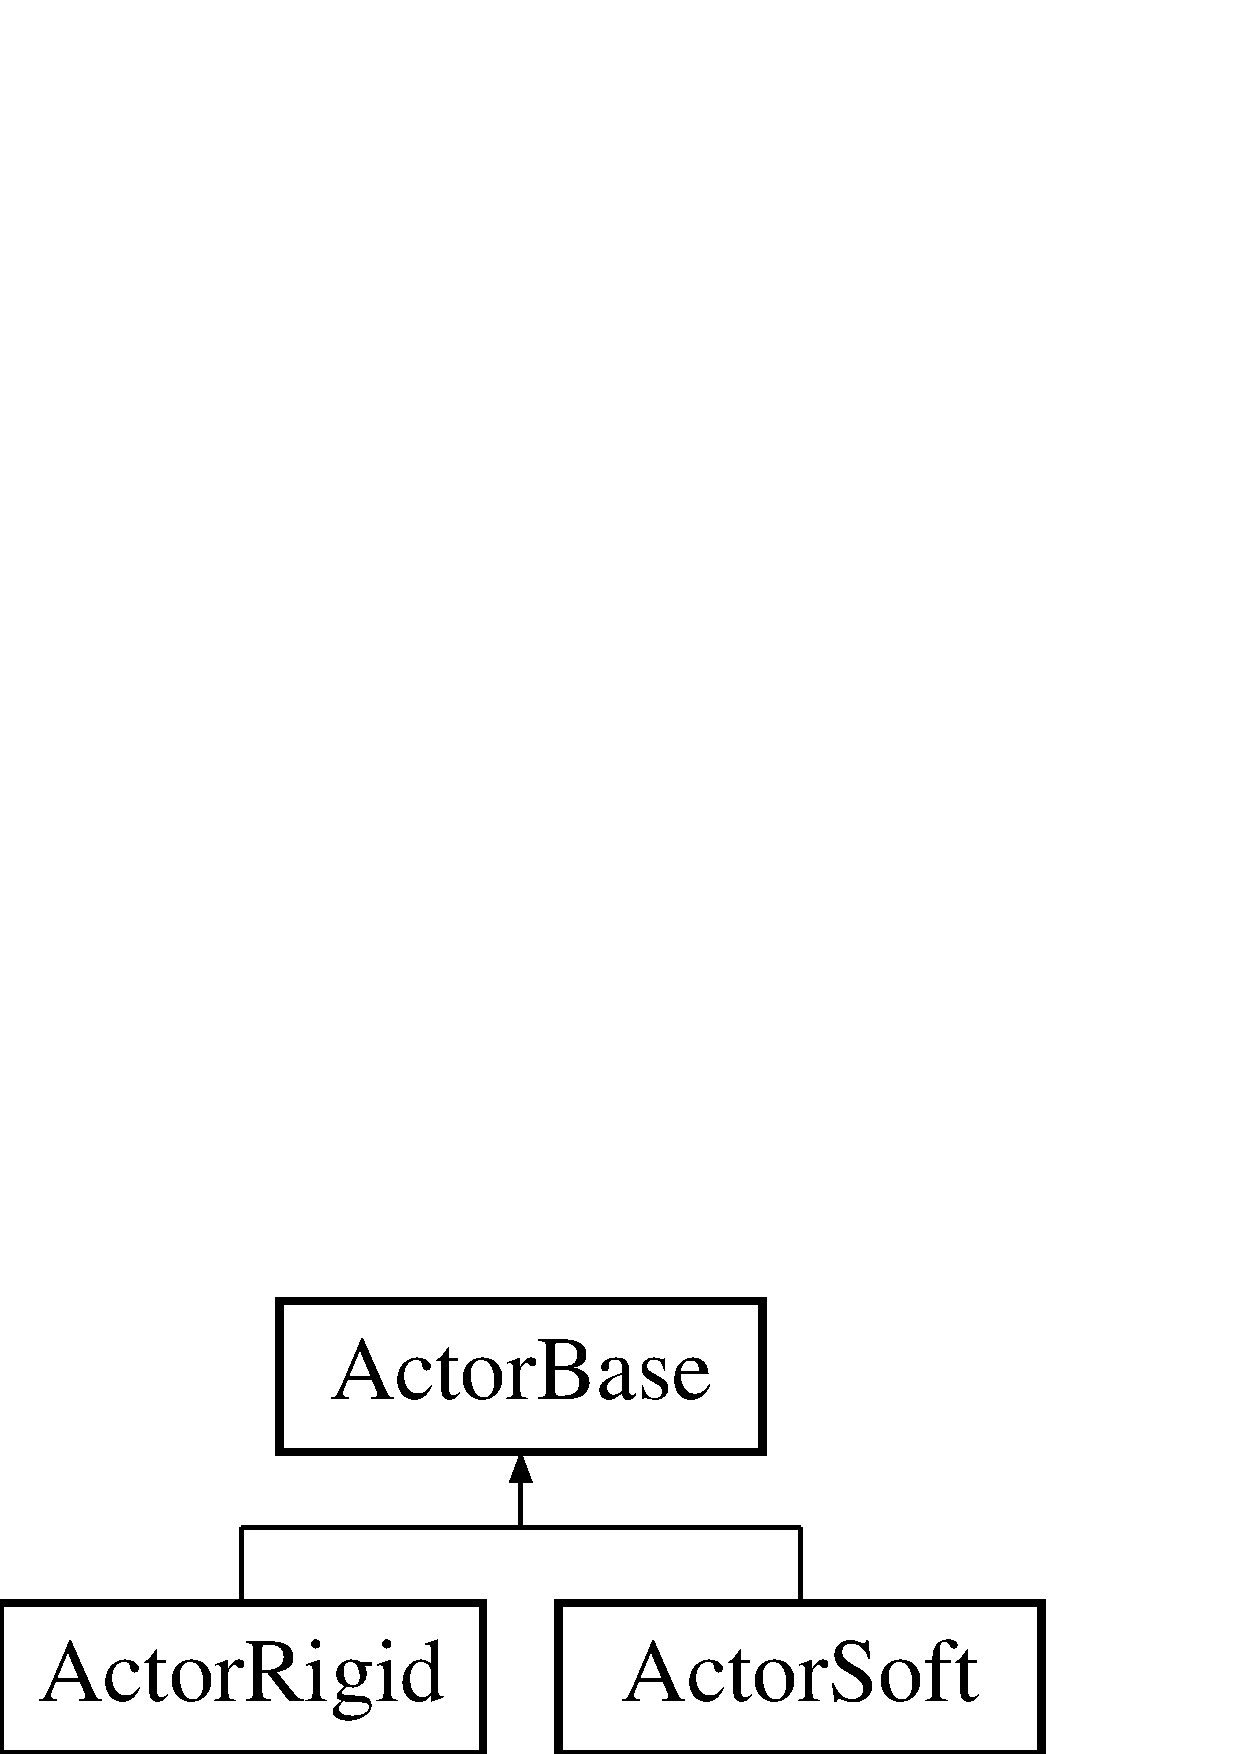
\includegraphics[height=2cm]{dd/d7b/classActorBase}
\end{center}
\end{figure}
\subsection*{Public Member Functions}
\begin{DoxyCompactItemize}
\item 
virtual \hyperlink{classActorBase_a6fd984c46b3232c2522adb44be4dedb7}{$\sim$ActorBase} ()
\begin{DoxyCompactList}\small\item\em Destructor. \item\end{DoxyCompactList}\item 
\hyperlink{classActorBase_a673d963aa7a99475cb03250c010dfa15}{ActorBase} (PhysString name, PhysString file, PhysString group, \hyperlink{classPhysWorld}{PhysWorld} $\ast$World)
\begin{DoxyCompactList}\small\item\em Descriptive constructor. \item\end{DoxyCompactList}\item 
void \hyperlink{classActorBase_a34848d620c5d9d2796999edbdcb77c9a}{SetLocation} (PhysReal x, PhysReal y, PhysReal z)
\begin{DoxyCompactList}\small\item\em Manually sets the location of the actor. \item\end{DoxyCompactList}\item 
void \hyperlink{classActorBase_a2a204add0b036de441ebd59d14939000}{SetLocation} (\hyperlink{classPhysVector3}{PhysVector3} Place)
\begin{DoxyCompactList}\small\item\em Manually sets the location of the actor. \item\end{DoxyCompactList}\item 
\hyperlink{classPhysVector3}{PhysVector3} \hyperlink{classActorBase_a9dfdaf0304e4a462b3b033fb254116af}{GetLocation} ()
\begin{DoxyCompactList}\small\item\em Retrieves the location of the object. \item\end{DoxyCompactList}\item 
void \hyperlink{classActorBase_ac118fc21f89d067d987d511b444f7d55}{SetInitLocation} (\hyperlink{classPhysVector3}{PhysVector3} Location)
\begin{DoxyCompactList}\small\item\em Sets the starting location of the actor. \item\end{DoxyCompactList}\item 
void \hyperlink{classActorBase_a72e2d0064c3e4c4d8937f490397a333f}{SetInitOrientation} (\hyperlink{classPhysQuaternion}{PhysQuaternion} Orientation)
\begin{DoxyCompactList}\small\item\em Sets the starting orientation of the actor. \item\end{DoxyCompactList}\item 
void \hyperlink{classActorBase_a9777506815a9840552b30c65d5d70f8d}{SetOrientation} (PhysReal x, PhysReal y, PhysReal z, PhysReal w)
\begin{DoxyCompactList}\small\item\em Sets the orientation of the actor. \item\end{DoxyCompactList}\item 
void \hyperlink{classActorBase_a5fe558ca0a88061615cda52a4dc5bf66}{SetOrientation} (\hyperlink{classPhysQuaternion}{PhysQuaternion} Rotation)
\begin{DoxyCompactList}\small\item\em Sets the orientation of the actor. \item\end{DoxyCompactList}\item 
void \hyperlink{classActorBase_a2d5f990e8c6925b7e44e9ec85f379e6a}{SetKinematic} ()
\begin{DoxyCompactList}\small\item\em Sets the state of the object to Kinematic. \item\end{DoxyCompactList}\item 
void \hyperlink{classActorBase_a97f55e5fff5d69483ebb0b9042a50bb0}{SetStatic} ()
\begin{DoxyCompactList}\small\item\em Sets the state of the object to Static. \item\end{DoxyCompactList}\end{DoxyCompactItemize}
\subsection*{Protected Member Functions}
\begin{DoxyCompactItemize}
\item 
virtual void \hyperlink{classActorBase_a1af82a2ed960fd114518fdf84d5ff146}{AddObjectToWorld} (\hyperlink{classPhysWorld}{PhysWorld} $\ast$TargetWorld, btSoftRigidDynamicsWorld $\ast$World)=0
\begin{DoxyCompactList}\small\item\em Adds the actor to the physics world. \item\end{DoxyCompactList}\item 
void \hyperlink{classActorBase_af7f0806222c79b5d5120dccefd93715e}{CreateTrimesh} ()
\begin{DoxyCompactList}\small\item\em Creates a trimesh shape from the mesh file. \item\end{DoxyCompactList}\item 
void \hyperlink{classActorBase_aa87583c47b8653e8ac7d96f1481b57fd}{CreateEntity} (PhysString name, PhysString file, PhysString group)
\begin{DoxyCompactList}\small\item\em Creates an entity for the mesh file to be placed on a scene node. \item\end{DoxyCompactList}\item 
void \hyperlink{classActorBase_a168cd57e20b2adfc5cae21627ddbae31}{CreateSceneNode} ()
\begin{DoxyCompactList}\small\item\em Creates a node for the entity in the graphical world. \item\end{DoxyCompactList}\item 
void \hyperlink{classActorBase_a3140cc5c1c630efc1c04c20ada319b8b}{SetOgreLocation} (\hyperlink{classPhysVector3}{PhysVector3} Place)
\begin{DoxyCompactList}\small\item\em Sets the location of the graphical body. \item\end{DoxyCompactList}\item 
\hyperlink{classPhysVector3}{PhysVector3} \hyperlink{classActorBase_a73ee03084b2ca78659b6e6439cafa75f}{GetOgreLocation} ()
\begin{DoxyCompactList}\small\item\em Retrieves the location of the graphical body. \item\end{DoxyCompactList}\item 
void \hyperlink{classActorBase_a55f45703e3d9b8de0cd07b23bd9460bf}{SetOgreOrientation} (\hyperlink{classPhysQuaternion}{PhysQuaternion} Rotation)
\begin{DoxyCompactList}\small\item\em Sets the orientation of the graphical body. \item\end{DoxyCompactList}\item 
void \hyperlink{classActorBase_afab604970fede16ccde0c6b8e72d9ee0}{AttachToGraphics} ()
\begin{DoxyCompactList}\small\item\em Makes the actor visable. \item\end{DoxyCompactList}\item 
virtual void \hyperlink{classActorBase_af64a57138bbd32c52581a5c8d0d29a76}{SetBulletLocation} (\hyperlink{classPhysVector3}{PhysVector3} Location)
\begin{DoxyCompactList}\small\item\em Sets the location of the physics body. \item\end{DoxyCompactList}\item 
virtual \hyperlink{classPhysVector3}{PhysVector3} \hyperlink{classActorBase_ae84ff822d2f962360bf291bb2c88eb3e}{GetBulletLocation} ()
\begin{DoxyCompactList}\small\item\em Retrieves the location of the physics body. \item\end{DoxyCompactList}\item 
void \hyperlink{classActorBase_af52177760d530df2b0987ed8626a656d}{SetBulletInitLocation} (\hyperlink{classPhysVector3}{PhysVector3} Location)
\begin{DoxyCompactList}\small\item\em Sets the starting location of the physics body within the \hyperlink{classPhysMotionState}{PhysMotionState}. \item\end{DoxyCompactList}\item 
virtual void \hyperlink{classActorBase_adf817bd5a7c562f31f6724a06a3a0f79}{SetBulletOrientation} (\hyperlink{classPhysQuaternion}{PhysQuaternion} Rotation)
\begin{DoxyCompactList}\small\item\em Sets the orientation of the physics body. \item\end{DoxyCompactList}\end{DoxyCompactItemize}
\subsection*{Protected Attributes}
\begin{DoxyCompactItemize}
\item 
\hypertarget{classActorBase_a02a4306818777f7c2e5853e8babd485e}{
\hyperlink{classPhysWorld}{PhysWorld} $\ast$ {\bfseries GameWorld}}
\label{dd/d7b/classActorBase_a02a4306818777f7c2e5853e8babd485e}

\item 
\hypertarget{classActorBase_ada6ceb752605b29357b6c5d53c477696}{
Ogre::Entity $\ast$ {\bfseries entity}}
\label{dd/d7b/classActorBase_ada6ceb752605b29357b6c5d53c477696}

\item 
\hypertarget{classActorBase_affa8851ae622e1d420afa4770ab89ea4}{
Ogre::SceneNode $\ast$ {\bfseries node}}
\label{dd/d7b/classActorBase_affa8851ae622e1d420afa4770ab89ea4}

\item 
\hypertarget{classActorBase_aff0d385bc9d30cf053838fd61b32ebad}{
btCollisionShape $\ast$ {\bfseries Shape}}
\label{dd/d7b/classActorBase_aff0d385bc9d30cf053838fd61b32ebad}

\item 
\hypertarget{classActorBase_ac4a1c0b5b5cd04f288f9614bfacb4fbe}{
btCollisionObject $\ast$ {\bfseries CollisionObject}}
\label{dd/d7b/classActorBase_ac4a1c0b5b5cd04f288f9614bfacb4fbe}

\item 
\hypertarget{classActorBase_a4ae7c4fd3b9449771e1c1bbd09cf103e}{
\hyperlink{classPhysMotionState}{PhysMotionState} $\ast$ {\bfseries MotionState}}
\label{dd/d7b/classActorBase_a4ae7c4fd3b9449771e1c1bbd09cf103e}

\end{DoxyCompactItemize}
\subsection*{Friends}
\begin{DoxyCompactItemize}
\item 
\hypertarget{classActorBase_a375fd37c70c941f0442997a60fdb05c7}{
class \hyperlink{classActorBase_a375fd37c70c941f0442997a60fdb05c7}{PhysWorld}}
\label{dd/d7b/classActorBase_a375fd37c70c941f0442997a60fdb05c7}

\end{DoxyCompactItemize}


\subsection{Detailed Description}
This is the base class from which all the actors inherit. The actor classes store and manage all the relevant data regarding objects inside the \hyperlink{classPhysWorld}{PhysWorld}. They serve as a binder between the physics and graphics for objects and have functions that allow the manipulation of objects loaded into the \hyperlink{classPhysWorld}{PhysWorld}. Currently there are 4 actor classes: \hyperlink{classActorBase}{ActorBase}, ActorDynRigid, ActorDynSoft, and ActorSta. \par
 \hyperlink{classActorBase}{ActorBase} is a base class that serves as a template for the other three actor classes. \par
 \hyperlink{classActorBase}{ActorBase} should never be created, as it lacks the functionality needed for most objects. 

Definition at line 88 of file physactor.h.



\subsection{Constructor \& Destructor Documentation}
\hypertarget{classActorBase_a6fd984c46b3232c2522adb44be4dedb7}{
\index{ActorBase@{ActorBase}!$\sim$ActorBase@{$\sim$ActorBase}}
\index{$\sim$ActorBase@{$\sim$ActorBase}!ActorBase@{ActorBase}}
\subsubsection[{$\sim$ActorBase}]{\setlength{\rightskip}{0pt plus 5cm}ActorBase::$\sim$ActorBase ()\hspace{0.3cm}{\ttfamily  \mbox{[}virtual\mbox{]}}}}
\label{dd/d7b/classActorBase_a6fd984c46b3232c2522adb44be4dedb7}


Destructor. 

The class destructor. 

Definition at line 114 of file physactor.cpp.

\hypertarget{classActorBase_a673d963aa7a99475cb03250c010dfa15}{
\index{ActorBase@{ActorBase}!ActorBase@{ActorBase}}
\index{ActorBase@{ActorBase}!ActorBase@{ActorBase}}
\subsubsection[{ActorBase}]{\setlength{\rightskip}{0pt plus 5cm}ActorBase::ActorBase (PhysString {\em name}, \/  PhysString {\em file}, \/  PhysString {\em group}, \/  {\bf PhysWorld} $\ast$ {\em World})}}
\label{dd/d7b/classActorBase_a673d963aa7a99475cb03250c010dfa15}


Descriptive constructor. 

This constructor contains the basic information needed to make an actor. 
\begin{DoxyParams}{Parameters}
\item[{\em Name}]The name of the actor. \item[{\em File}]The 3d mesh file that contains the 3d model the actor will use. \item[{\em Group}]The resource group where the 3d mesh and other related files can be found. \item[{\em World}]Pointer to the \hyperlink{classPhysWorld}{PhysWorld} this object will be added to. \end{DoxyParams}


Definition at line 104 of file physactor.cpp.



\subsection{Member Function Documentation}
\hypertarget{classActorBase_a1af82a2ed960fd114518fdf84d5ff146}{
\index{ActorBase@{ActorBase}!AddObjectToWorld@{AddObjectToWorld}}
\index{AddObjectToWorld@{AddObjectToWorld}!ActorBase@{ActorBase}}
\subsubsection[{AddObjectToWorld}]{\setlength{\rightskip}{0pt plus 5cm}virtual void ActorBase::AddObjectToWorld ({\bf PhysWorld} $\ast$ {\em TargetWorld}, \/  btSoftRigidDynamicsWorld $\ast$ {\em World})\hspace{0.3cm}{\ttfamily  \mbox{[}protected, pure virtual\mbox{]}}}}
\label{dd/d7b/classActorBase_a1af82a2ed960fd114518fdf84d5ff146}


Adds the actor to the physics world. 

Adds the actor to the physics world. \par
 This is automaticly called by the PhysWorlds AddActor function and shouldn't be called manually. 
\begin{DoxyParams}{Parameters}
\item[{\em TargetWorld}]Pointer to the \hyperlink{classPhysWorld}{PhysWorld} class. \item[{\em World}]Pointer to the physics world. \end{DoxyParams}


Implemented in \hyperlink{classActorRigid_ac6d7e05944623329f0c2140c19e2c49e}{ActorRigid}, and \hyperlink{classActorSoft_a0def29f28ed4d126a0634ddc97e33e2f}{ActorSoft}.

\hypertarget{classActorBase_afab604970fede16ccde0c6b8e72d9ee0}{
\index{ActorBase@{ActorBase}!AttachToGraphics@{AttachToGraphics}}
\index{AttachToGraphics@{AttachToGraphics}!ActorBase@{ActorBase}}
\subsubsection[{AttachToGraphics}]{\setlength{\rightskip}{0pt plus 5cm}void ActorBase::AttachToGraphics ()\hspace{0.3cm}{\ttfamily  \mbox{[}protected\mbox{]}}}}
\label{dd/d7b/classActorBase_afab604970fede16ccde0c6b8e72d9ee0}


Makes the actor visable. 

Adds the actor to all the nessessary graphics elements to make it visable on screen. \par
 This is automaticly called by the PhysWorlds AddActor function and shouldn't ever need to be called manually. 

Definition at line 313 of file physactor.cpp.

\hypertarget{classActorBase_aa87583c47b8653e8ac7d96f1481b57fd}{
\index{ActorBase@{ActorBase}!CreateEntity@{CreateEntity}}
\index{CreateEntity@{CreateEntity}!ActorBase@{ActorBase}}
\subsubsection[{CreateEntity}]{\setlength{\rightskip}{0pt plus 5cm}void ActorBase::CreateEntity (PhysString {\em name}, \/  PhysString {\em file}, \/  PhysString {\em group})\hspace{0.3cm}{\ttfamily  \mbox{[}protected\mbox{]}}}}
\label{dd/d7b/classActorBase_aa87583c47b8653e8ac7d96f1481b57fd}


Creates an entity for the mesh file to be placed on a scene node. 

Creates an entity in the scene manager from the mesh file provided to be attached to a node in the graphical world. \par
 This function is called on by the Constructor, and shouldn't be called manually. 
\begin{DoxyParams}{Parameters}
\item[{\em Name}]Name of the actor. \item[{\em File}]File name of the graphical mesh to be used. \item[{\em Group}]Resource group where the graphical mesh can be found. \end{DoxyParams}


Definition at line 222 of file physactor.cpp.

\hypertarget{classActorBase_a168cd57e20b2adfc5cae21627ddbae31}{
\index{ActorBase@{ActorBase}!CreateSceneNode@{CreateSceneNode}}
\index{CreateSceneNode@{CreateSceneNode}!ActorBase@{ActorBase}}
\subsubsection[{CreateSceneNode}]{\setlength{\rightskip}{0pt plus 5cm}void ActorBase::CreateSceneNode ()\hspace{0.3cm}{\ttfamily  \mbox{[}protected\mbox{]}}}}
\label{dd/d7b/classActorBase_a168cd57e20b2adfc5cae21627ddbae31}


Creates a node for the entity in the graphical world. 

Creates a node in the scene manager to attach the actor's entity to within the graphical world. \par
 This function is called on by the Constructor, and shouldn't be called manually. 

Definition at line 227 of file physactor.cpp.

\hypertarget{classActorBase_af7f0806222c79b5d5120dccefd93715e}{
\index{ActorBase@{ActorBase}!CreateTrimesh@{CreateTrimesh}}
\index{CreateTrimesh@{CreateTrimesh}!ActorBase@{ActorBase}}
\subsubsection[{CreateTrimesh}]{\setlength{\rightskip}{0pt plus 5cm}void ActorBase::CreateTrimesh ()\hspace{0.3cm}{\ttfamily  \mbox{[}protected\mbox{]}}}}
\label{dd/d7b/classActorBase_af7f0806222c79b5d5120dccefd93715e}


Creates a trimesh shape from the mesh file. 

Makes a trimesh to be used as a collision shape in the physics world from a mesh file. \par
 This is automaticly called by the CreateShapeFromMesh function in child classes and shouldn't be called manually. 

TODO -\/ Check for thread safety 



Definition at line 120 of file physactor.cpp.

\hypertarget{classActorBase_ae84ff822d2f962360bf291bb2c88eb3e}{
\index{ActorBase@{ActorBase}!GetBulletLocation@{GetBulletLocation}}
\index{GetBulletLocation@{GetBulletLocation}!ActorBase@{ActorBase}}
\subsubsection[{GetBulletLocation}]{\setlength{\rightskip}{0pt plus 5cm}{\bf PhysVector3} ActorBase::GetBulletLocation ()\hspace{0.3cm}{\ttfamily  \mbox{[}protected, virtual\mbox{]}}}}
\label{dd/d7b/classActorBase_ae84ff822d2f962360bf291bb2c88eb3e}


Retrieves the location of the physics body. 

This function will retrieve the location of the object within the physics world. 

Definition at line 250 of file physactor.cpp.

\hypertarget{classActorBase_a9dfdaf0304e4a462b3b033fb254116af}{
\index{ActorBase@{ActorBase}!GetLocation@{GetLocation}}
\index{GetLocation@{GetLocation}!ActorBase@{ActorBase}}
\subsubsection[{GetLocation}]{\setlength{\rightskip}{0pt plus 5cm}{\bf PhysVector3} ActorBase::GetLocation ()}}
\label{dd/d7b/classActorBase_a9dfdaf0304e4a462b3b033fb254116af}


Retrieves the location of the object. 

This function will retrieve the location of the object within the world. 

Definition at line 286 of file physactor.cpp.

\hypertarget{classActorBase_a73ee03084b2ca78659b6e6439cafa75f}{
\index{ActorBase@{ActorBase}!GetOgreLocation@{GetOgreLocation}}
\index{GetOgreLocation@{GetOgreLocation}!ActorBase@{ActorBase}}
\subsubsection[{GetOgreLocation}]{\setlength{\rightskip}{0pt plus 5cm}{\bf PhysVector3} ActorBase::GetOgreLocation ()\hspace{0.3cm}{\ttfamily  \mbox{[}protected\mbox{]}}}}
\label{dd/d7b/classActorBase_a73ee03084b2ca78659b6e6439cafa75f}


Retrieves the location of the graphical body. 

This function will retrieve the location of the object within the graphical world. 

Definition at line 237 of file physactor.cpp.

\hypertarget{classActorBase_af52177760d530df2b0987ed8626a656d}{
\index{ActorBase@{ActorBase}!SetBulletInitLocation@{SetBulletInitLocation}}
\index{SetBulletInitLocation@{SetBulletInitLocation}!ActorBase@{ActorBase}}
\subsubsection[{SetBulletInitLocation}]{\setlength{\rightskip}{0pt plus 5cm}void ActorBase::SetBulletInitLocation ({\bf PhysVector3} {\em Location})\hspace{0.3cm}{\ttfamily  \mbox{[}protected\mbox{]}}}}
\label{dd/d7b/classActorBase_af52177760d530df2b0987ed8626a656d}


Sets the starting location of the physics body within the \hyperlink{classPhysMotionState}{PhysMotionState}. 

Sets the starting location of the physics body within the \hyperlink{classPhysMotionState}{PhysMotionState}. \par
 This function is called on by the SetInitLocation function, and shouldn't be called manually. 
\begin{DoxyParams}{Parameters}
\item[{\em Location}]The \hyperlink{classPhysVector3}{PhysVector3} representing the desired starting location for the actor. \end{DoxyParams}


Definition at line 258 of file physactor.cpp.

\hypertarget{classActorBase_af64a57138bbd32c52581a5c8d0d29a76}{
\index{ActorBase@{ActorBase}!SetBulletLocation@{SetBulletLocation}}
\index{SetBulletLocation@{SetBulletLocation}!ActorBase@{ActorBase}}
\subsubsection[{SetBulletLocation}]{\setlength{\rightskip}{0pt plus 5cm}void ActorBase::SetBulletLocation ({\bf PhysVector3} {\em Location})\hspace{0.3cm}{\ttfamily  \mbox{[}protected, virtual\mbox{]}}}}
\label{dd/d7b/classActorBase_af64a57138bbd32c52581a5c8d0d29a76}


Sets the location of the physics body. 

This will take a \hyperlink{classPhysVector3}{PhysVector3} and set the location of the actor within the physics world. \par
 This function is called on by the SetLocation function, and shouldn't be called manually. 
\begin{DoxyParams}{Parameters}
\item[{\em Location}]The \hyperlink{classPhysVector3}{PhysVector3} representing the location. \end{DoxyParams}


Definition at line 244 of file physactor.cpp.

\hypertarget{classActorBase_adf817bd5a7c562f31f6724a06a3a0f79}{
\index{ActorBase@{ActorBase}!SetBulletOrientation@{SetBulletOrientation}}
\index{SetBulletOrientation@{SetBulletOrientation}!ActorBase@{ActorBase}}
\subsubsection[{SetBulletOrientation}]{\setlength{\rightskip}{0pt plus 5cm}void ActorBase::SetBulletOrientation ({\bf PhysQuaternion} {\em Rotation})\hspace{0.3cm}{\ttfamily  \mbox{[}protected, virtual\mbox{]}}}}
\label{dd/d7b/classActorBase_adf817bd5a7c562f31f6724a06a3a0f79}


Sets the orientation of the physics body. 

This will take a \hyperlink{classPhysQuaternion}{PhysQuaternion} and set the orientation of the actor within the physics world. \par
 This function is called on by the SetOrientation function, and shouldn't be called manually. 
\begin{DoxyParams}{Parameters}
\item[{\em Rotation}]The quaternion representing the rotation of the actor. \end{DoxyParams}


Definition at line 268 of file physactor.cpp.

\hypertarget{classActorBase_ac118fc21f89d067d987d511b444f7d55}{
\index{ActorBase@{ActorBase}!SetInitLocation@{SetInitLocation}}
\index{SetInitLocation@{SetInitLocation}!ActorBase@{ActorBase}}
\subsubsection[{SetInitLocation}]{\setlength{\rightskip}{0pt plus 5cm}void ActorBase::SetInitLocation ({\bf PhysVector3} {\em Location})}}
\label{dd/d7b/classActorBase_ac118fc21f89d067d987d511b444f7d55}


Sets the starting location of the actor. 

Calling this function after adding it to the \hyperlink{classPhysWorld}{PhysWorld} will have no effect. \par
 This function will set where the actor will be located in the \hyperlink{classPhysWorld}{PhysWorld} when it is first placed inside the world. 
\begin{DoxyParams}{Parameters}
\item[{\em Location}]The \hyperlink{classPhysVector3}{PhysVector3} representing the location. \end{DoxyParams}


Definition at line 291 of file physactor.cpp.

\hypertarget{classActorBase_a72e2d0064c3e4c4d8937f490397a333f}{
\index{ActorBase@{ActorBase}!SetInitOrientation@{SetInitOrientation}}
\index{SetInitOrientation@{SetInitOrientation}!ActorBase@{ActorBase}}
\subsubsection[{SetInitOrientation}]{\setlength{\rightskip}{0pt plus 5cm}void ActorBase::SetInitOrientation ({\bf PhysQuaternion} {\em Orientation})}}
\label{dd/d7b/classActorBase_a72e2d0064c3e4c4d8937f490397a333f}


Sets the starting orientation of the actor. 

Calling this function after adding it to the \hyperlink{classPhysWorld}{PhysWorld} will have no effect. \par
 This function will set where the actor is facing in the \hyperlink{classPhysWorld}{PhysWorld} when it is first placed inside the world. 
\begin{DoxyParams}{Parameters}
\item[{\em Orientation}]The \hyperlink{classPhysQuaternion}{PhysQuaternion} representing the Orientation. \end{DoxyParams}


Definition at line 296 of file physactor.cpp.

\hypertarget{classActorBase_a2d5f990e8c6925b7e44e9ec85f379e6a}{
\index{ActorBase@{ActorBase}!SetKinematic@{SetKinematic}}
\index{SetKinematic@{SetKinematic}!ActorBase@{ActorBase}}
\subsubsection[{SetKinematic}]{\setlength{\rightskip}{0pt plus 5cm}void ActorBase::SetKinematic ()}}
\label{dd/d7b/classActorBase_a2d5f990e8c6925b7e44e9ec85f379e6a}


Sets the state of the object to Kinematic. 

This function will set the object to a Kinematic Object. \par
 Kinematic Objects are like Static Objects but are also able to be moved directly by character controllers. 

Definition at line 321 of file physactor.cpp.

\hypertarget{classActorBase_a2a204add0b036de441ebd59d14939000}{
\index{ActorBase@{ActorBase}!SetLocation@{SetLocation}}
\index{SetLocation@{SetLocation}!ActorBase@{ActorBase}}
\subsubsection[{SetLocation}]{\setlength{\rightskip}{0pt plus 5cm}void ActorBase::SetLocation ({\bf PhysVector3} {\em Place})}}
\label{dd/d7b/classActorBase_a2a204add0b036de441ebd59d14939000}


Manually sets the location of the actor. 

Calling this function prior to adding it to the \hyperlink{classPhysWorld}{PhysWorld} will have no effect. \par
 In most situations you won't want to use this function, and instead produce movement through physics functions. 
\begin{DoxyParams}{Parameters}
\item[{\em Place}]The \hyperlink{classPhysVector3}{PhysVector3} representing the location. \end{DoxyParams}


Definition at line 280 of file physactor.cpp.

\hypertarget{classActorBase_a34848d620c5d9d2796999edbdcb77c9a}{
\index{ActorBase@{ActorBase}!SetLocation@{SetLocation}}
\index{SetLocation@{SetLocation}!ActorBase@{ActorBase}}
\subsubsection[{SetLocation}]{\setlength{\rightskip}{0pt plus 5cm}void ActorBase::SetLocation (PhysReal {\em x}, \/  PhysReal {\em y}, \/  PhysReal {\em z})}}
\label{dd/d7b/classActorBase_a34848d620c5d9d2796999edbdcb77c9a}


Manually sets the location of the actor. 

Calling this function prior to adding it to the \hyperlink{classPhysWorld}{PhysWorld} will have no effect. \par
 In most situations you won't want to use this function, and instead produce movement through physics functions. 
\begin{DoxyParams}{Parameters}
\item[{\em X}]Location on the X vector. \item[{\em Y}]Location on the Y vector. \item[{\em Z}]Location on the Z vector. \end{DoxyParams}


Definition at line 274 of file physactor.cpp.

\hypertarget{classActorBase_a3140cc5c1c630efc1c04c20ada319b8b}{
\index{ActorBase@{ActorBase}!SetOgreLocation@{SetOgreLocation}}
\index{SetOgreLocation@{SetOgreLocation}!ActorBase@{ActorBase}}
\subsubsection[{SetOgreLocation}]{\setlength{\rightskip}{0pt plus 5cm}void ActorBase::SetOgreLocation ({\bf PhysVector3} {\em Place})\hspace{0.3cm}{\ttfamily  \mbox{[}protected\mbox{]}}}}
\label{dd/d7b/classActorBase_a3140cc5c1c630efc1c04c20ada319b8b}


Sets the location of the graphical body. 

This will take a \hyperlink{classPhysVector3}{PhysVector3} and set the location of the actor within the graphical world. \par
 This function is called on by the SetLocation function, and shouldn't be called manually. 
\begin{DoxyParams}{Parameters}
\item[{\em Location}]The \hyperlink{classPhysVector3}{PhysVector3} representing the location. \end{DoxyParams}


Definition at line 232 of file physactor.cpp.

\hypertarget{classActorBase_a55f45703e3d9b8de0cd07b23bd9460bf}{
\index{ActorBase@{ActorBase}!SetOgreOrientation@{SetOgreOrientation}}
\index{SetOgreOrientation@{SetOgreOrientation}!ActorBase@{ActorBase}}
\subsubsection[{SetOgreOrientation}]{\setlength{\rightskip}{0pt plus 5cm}void ActorBase::SetOgreOrientation ({\bf PhysQuaternion} {\em Rotation})\hspace{0.3cm}{\ttfamily  \mbox{[}protected\mbox{]}}}}
\label{dd/d7b/classActorBase_a55f45703e3d9b8de0cd07b23bd9460bf}


Sets the orientation of the graphical body. 

This will take a \hyperlink{classPhysQuaternion}{PhysQuaternion} and set the orientation of the actor within the graphical world. \par
 This function is called on by the SetOrientation function, and shouldn't be called manually. 
\begin{DoxyParams}{Parameters}
\item[{\em Rotation}]The quaternion representing the rotation of the actor. \end{DoxyParams}


Definition at line 263 of file physactor.cpp.

\hypertarget{classActorBase_a5fe558ca0a88061615cda52a4dc5bf66}{
\index{ActorBase@{ActorBase}!SetOrientation@{SetOrientation}}
\index{SetOrientation@{SetOrientation}!ActorBase@{ActorBase}}
\subsubsection[{SetOrientation}]{\setlength{\rightskip}{0pt plus 5cm}void ActorBase::SetOrientation ({\bf PhysQuaternion} {\em Rotation})}}
\label{dd/d7b/classActorBase_a5fe558ca0a88061615cda52a4dc5bf66}


Sets the orientation of the actor. 

Sets the orientation of the actor via a Quaternion. 
\begin{DoxyParams}{Parameters}
\item[{\em Rotation}]The Quaternion representing the Rotation. \end{DoxyParams}


Definition at line 307 of file physactor.cpp.

\hypertarget{classActorBase_a9777506815a9840552b30c65d5d70f8d}{
\index{ActorBase@{ActorBase}!SetOrientation@{SetOrientation}}
\index{SetOrientation@{SetOrientation}!ActorBase@{ActorBase}}
\subsubsection[{SetOrientation}]{\setlength{\rightskip}{0pt plus 5cm}void ActorBase::SetOrientation (PhysReal {\em x}, \/  PhysReal {\em y}, \/  PhysReal {\em z}, \/  PhysReal {\em w})}}
\label{dd/d7b/classActorBase_a9777506815a9840552b30c65d5d70f8d}


Sets the orientation of the actor. 

Sets the orientation of the actor via Quaternion parameters. 

Definition at line 301 of file physactor.cpp.

\hypertarget{classActorBase_a97f55e5fff5d69483ebb0b9042a50bb0}{
\index{ActorBase@{ActorBase}!SetStatic@{SetStatic}}
\index{SetStatic@{SetStatic}!ActorBase@{ActorBase}}
\subsubsection[{SetStatic}]{\setlength{\rightskip}{0pt plus 5cm}void ActorBase::SetStatic ()}}
\label{dd/d7b/classActorBase_a97f55e5fff5d69483ebb0b9042a50bb0}


Sets the state of the object to Static. 

This function will set the object to a Static Object. \par
 Static Objects don't move or have any force applied to them, but are cabable of exerting force on other objects. 

Definition at line 327 of file physactor.cpp.



The documentation for this class was generated from the following files:\begin{DoxyCompactItemize}
\item 
physactor.h\item 
physactor.cpp\end{DoxyCompactItemize}

\hypertarget{classActorDynRigid}{
\section{ActorDynRigid Class Reference}
\label{d4/d0e/classActorDynRigid}\index{ActorDynRigid@{ActorDynRigid}}
}
Inheritance diagram for ActorDynRigid::\begin{figure}[H]
\begin{center}
\leavevmode
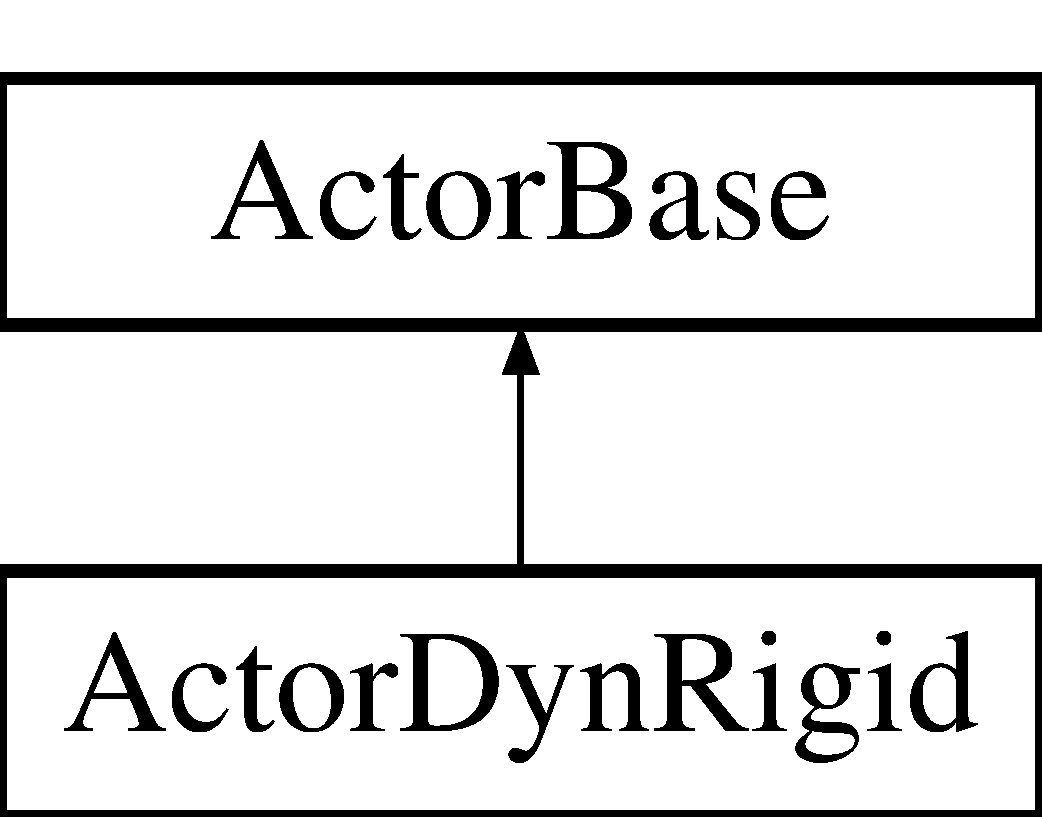
\includegraphics[height=2cm]{d4/d0e/classActorDynRigid}
\end{center}
\end{figure}
\subsection*{Public Member Functions}
\begin{DoxyCompactItemize}
\item 
\hypertarget{classActorDynRigid_aa537dd154a64e34d5c08f660affc4300}{
void {\bfseries CreateRigidObject} ()}
\label{d4/d0e/classActorDynRigid_aa537dd154a64e34d5c08f660affc4300}

\item 
\hypertarget{classActorDynRigid_a5677d046cf6d0bbc6992b93e10290e6c}{
void {\bfseries AddObjectToWorld} ()}
\label{d4/d0e/classActorDynRigid_a5677d046cf6d0bbc6992b93e10290e6c}

\end{DoxyCompactItemize}
\subsection*{Protected Attributes}
\begin{DoxyCompactItemize}
\item 
\hypertarget{classActorDynRigid_a83a6cb758304431043c6bfa05b47ecb2}{
btRigidBody $\ast$ {\bfseries physrigidbody}}
\label{d4/d0e/classActorDynRigid_a83a6cb758304431043c6bfa05b47ecb2}

\item 
\hypertarget{classActorDynRigid_a25c39b4f28cb2516511838a66f6eb3d8}{
btMotionState $\ast$ {\bfseries physmotionstate}}
\label{d4/d0e/classActorDynRigid_a25c39b4f28cb2516511838a66f6eb3d8}

\end{DoxyCompactItemize}


\subsection{Detailed Description}


Definition at line 47 of file physactor.h.

The documentation for this class was generated from the following files:\begin{DoxyCompactItemize}
\item 
physactor.h\item 
physactor.cpp\end{DoxyCompactItemize}

\hypertarget{classActorDynSoft}{
\section{ActorDynSoft Class Reference}
\label{dc/de0/classActorDynSoft}\index{ActorDynSoft@{ActorDynSoft}}
}
Inheritance diagram for ActorDynSoft::\begin{figure}[H]
\begin{center}
\leavevmode
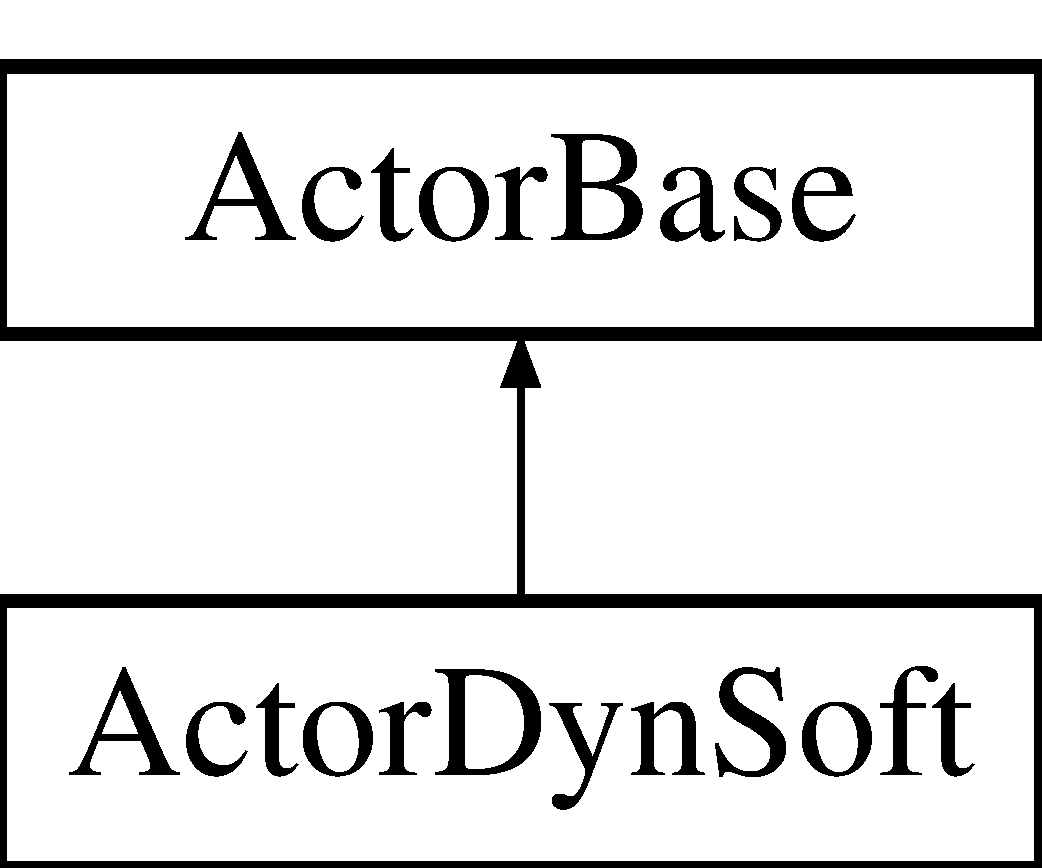
\includegraphics[height=2cm]{dc/de0/classActorDynSoft}
\end{center}
\end{figure}
\subsection*{Public Member Functions}
\begin{DoxyCompactItemize}
\item 
\hypertarget{classActorDynSoft_a249bc0621b1d55ea0a9c7787605078d6}{
void {\bfseries CreateSoftObject} ()}
\label{dc/de0/classActorDynSoft_a249bc0621b1d55ea0a9c7787605078d6}

\end{DoxyCompactItemize}
\subsection*{Protected Member Functions}
\begin{DoxyCompactItemize}
\item 
\hypertarget{classActorDynSoft_a6bd52511d954edfe09c26594535dd2f1}{
void {\bfseries AddObjectToWorld} (\hyperlink{classPhysWorld}{PhysWorld} $\ast$TargetWorld, btDiscreteDynamicsWorld $\ast$TargetPhysicsWorld)}
\label{dc/de0/classActorDynSoft_a6bd52511d954edfe09c26594535dd2f1}

\end{DoxyCompactItemize}
\subsection*{Protected Attributes}
\begin{DoxyCompactItemize}
\item 
\hypertarget{classActorDynSoft_a9f5b3e1cfa400bb6095f77feb81e76d8}{
btSoftBody $\ast$ {\bfseries physoftbody}}
\label{dc/de0/classActorDynSoft_a9f5b3e1cfa400bb6095f77feb81e76d8}

\item 
\hypertarget{classActorDynSoft_aad9dfc6f0d3f08c8abd110c8c9175b97}{
btMotionState $\ast$ {\bfseries physmotionstate}}
\label{dc/de0/classActorDynSoft_aad9dfc6f0d3f08c8abd110c8c9175b97}

\end{DoxyCompactItemize}


\subsection{Detailed Description}


Definition at line 85 of file physactor.h.

The documentation for this class was generated from the following files:\begin{DoxyCompactItemize}
\item 
physactor.h\item 
physactor.cpp\end{DoxyCompactItemize}

\hypertarget{classActorSta}{
\section{ActorSta Class Reference}
\label{d3/daf/classActorSta}\index{ActorSta@{ActorSta}}
}


This is the actor class for Static and Kinematic Objects.  


{\ttfamily \#include $<$physactor.h$>$}Inheritance diagram for ActorSta::\begin{figure}[H]
\begin{center}
\leavevmode
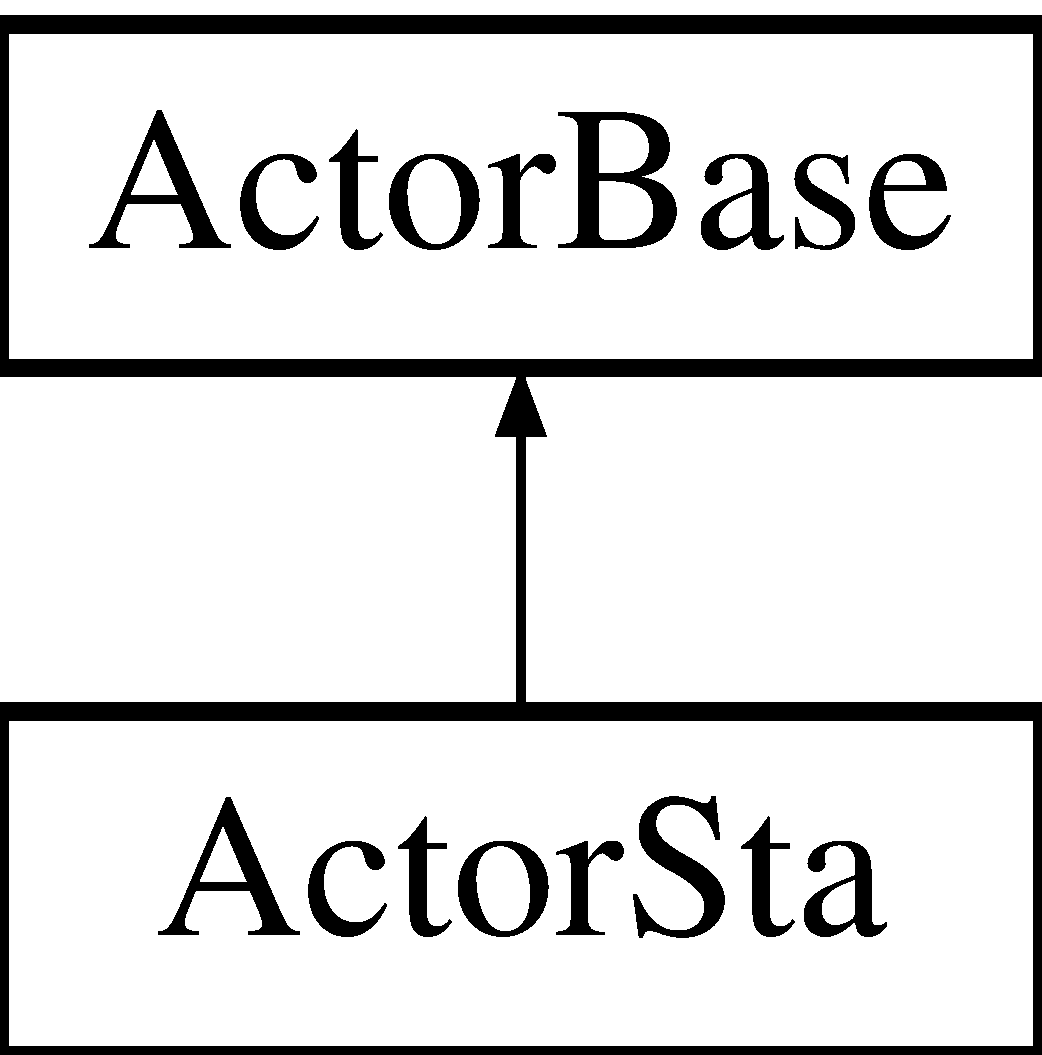
\includegraphics[height=2cm]{d3/daf/classActorSta}
\end{center}
\end{figure}
\subsection*{Public Member Functions}
\begin{DoxyCompactItemize}
\item 
\hyperlink{classActorSta_a00185fe588416c236f491b65f16dd145}{ActorSta} (PhysString name, PhysString file, PhysString group, \hyperlink{classPhysWorld}{PhysWorld} $\ast$World)
\begin{DoxyCompactList}\small\item\em Descriptive constructor. \item\end{DoxyCompactList}\item 
virtual \hyperlink{classActorSta_a5da54cd102413f920df2dae3555fead2}{$\sim$ActorSta} ()
\begin{DoxyCompactList}\small\item\em Destructor. \item\end{DoxyCompactList}\item 
void \hyperlink{classActorSta_a12e78aa21e50e6964330e25affa421c9}{CreateShapeFromMesh} ()
\begin{DoxyCompactList}\small\item\em Creates a collision shape from mesh file. \item\end{DoxyCompactList}\end{DoxyCompactItemize}
\subsection*{Protected Member Functions}
\begin{DoxyCompactItemize}
\item 
void \hyperlink{classActorSta_ae856b69de748541606649d21d2e6c270}{CreateRigidObject} ()
\begin{DoxyCompactList}\small\item\em Creates a rigid object for the actor. \item\end{DoxyCompactList}\item 
void \hyperlink{classActorSta_acd11f1ee404ab71d49d8fd4a810f2931}{AddObjectToWorld} (\hyperlink{classPhysWorld}{PhysWorld} $\ast$TargetWorld, btSoftRigidDynamicsWorld $\ast$World)
\begin{DoxyCompactList}\small\item\em Adds the actor to the physics world. \item\end{DoxyCompactList}\item 
virtual void \hyperlink{classActorSta_a472768e39d3ac67f35b9f74e5a679b99}{SetBulletLocation} (\hyperlink{classPhysVector3}{PhysVector3} Location)
\begin{DoxyCompactList}\small\item\em Sets the location of the physics body. \item\end{DoxyCompactList}\item 
virtual void \hyperlink{classActorSta_ab038b2ce4e25fa3441e9b081cef7879e}{SetBulletOrientation} (\hyperlink{classPhysQuaternion}{PhysQuaternion} Rotation)
\begin{DoxyCompactList}\small\item\em Sets the orientation of the physics body. \item\end{DoxyCompactList}\end{DoxyCompactItemize}
\subsection*{Protected Attributes}
\begin{DoxyCompactItemize}
\item 
\hypertarget{classActorSta_ad12363fc4cd60d6cdd5e3c6d36d96f20}{
btRigidBody $\ast$ {\bfseries physrigidbody}}
\label{d3/daf/classActorSta_ad12363fc4cd60d6cdd5e3c6d36d96f20}

\end{DoxyCompactItemize}


\subsection{Detailed Description}
This is the actor class for Static and Kinematic Objects. This class should be used to make any object that you do not want to have move as a result of force from another object, or any other physics related force. A basic static object is an object that sits in one location exerting force on others that collide with it but don't move themselves. Kinematic objects are the same as static objects but also have functions to allow it to be moved around manually by the game or programmer. 

Definition at line 305 of file physactor.h.

\subsection{Constructor \& Destructor Documentation}
\hypertarget{classActorSta_a00185fe588416c236f491b65f16dd145}{
\index{ActorSta@{ActorSta}!ActorSta@{ActorSta}}
\index{ActorSta@{ActorSta}!ActorSta@{ActorSta}}
\subsubsection[{ActorSta}]{\setlength{\rightskip}{0pt plus 5cm}ActorSta::ActorSta (PhysString {\em name}, \/  PhysString {\em file}, \/  PhysString {\em group}, \/  {\bf PhysWorld} $\ast$ {\em World})}}
\label{d3/daf/classActorSta_a00185fe588416c236f491b65f16dd145}


Descriptive constructor. This constructor contains the basic information needed to make a Static or Kinematic Rigid Object. \par
 This class inherits from \hyperlink{classActorBase}{ActorBase}. Mass is always zero for Static/Kinematic Objects.` 
\begin{DoxyParams}{Parameters}
\item[{\em Name}]The name of the actor. \item[{\em File}]The 3d mesh file that contains the 3d model the actor will use. \item[{\em Group}]The resource group where the 3d mesh and other related files can be found. \item[{\em World}]Pointer to the \hyperlink{classPhysWorld}{PhysWorld} this object will be added to. \end{DoxyParams}


Definition at line 350 of file physactor.cpp.\hypertarget{classActorSta_a5da54cd102413f920df2dae3555fead2}{
\index{ActorSta@{ActorSta}!$\sim$ActorSta@{$\sim$ActorSta}}
\index{$\sim$ActorSta@{$\sim$ActorSta}!ActorSta@{ActorSta}}
\subsubsection[{$\sim$ActorSta}]{\setlength{\rightskip}{0pt plus 5cm}ActorSta::$\sim$ActorSta ()\hspace{0.3cm}{\ttfamily  \mbox{[}virtual\mbox{]}}}}
\label{d3/daf/classActorSta_a5da54cd102413f920df2dae3555fead2}


Destructor. The class destructor. 

Definition at line 355 of file physactor.cpp.

\subsection{Member Function Documentation}
\hypertarget{classActorSta_acd11f1ee404ab71d49d8fd4a810f2931}{
\index{ActorSta@{ActorSta}!AddObjectToWorld@{AddObjectToWorld}}
\index{AddObjectToWorld@{AddObjectToWorld}!ActorSta@{ActorSta}}
\subsubsection[{AddObjectToWorld}]{\setlength{\rightskip}{0pt plus 5cm}void ActorSta::AddObjectToWorld ({\bf PhysWorld} $\ast$ {\em TargetWorld}, \/  btSoftRigidDynamicsWorld $\ast$ {\em World})\hspace{0.3cm}{\ttfamily  \mbox{[}protected, virtual\mbox{]}}}}
\label{d3/daf/classActorSta_acd11f1ee404ab71d49d8fd4a810f2931}


Adds the actor to the physics world. Adds the actor to the physics world. \par
 This is automaticly called by the PhysWorlds AddActor function and shouldn't be called manually. 
\begin{DoxyParams}{Parameters}
\item[{\em TargetWorld}]Pointer to the \hyperlink{classPhysWorld}{PhysWorld} class. \item[{\em World}]Pointer to the physics world. \end{DoxyParams}


Implements \hyperlink{classActorBase_a1af82a2ed960fd114518fdf84d5ff146}{ActorBase}.

Definition at line 366 of file physactor.cpp.\hypertarget{classActorSta_ae856b69de748541606649d21d2e6c270}{
\index{ActorSta@{ActorSta}!CreateRigidObject@{CreateRigidObject}}
\index{CreateRigidObject@{CreateRigidObject}!ActorSta@{ActorSta}}
\subsubsection[{CreateRigidObject}]{\setlength{\rightskip}{0pt plus 5cm}void ActorSta::CreateRigidObject ()\hspace{0.3cm}{\ttfamily  \mbox{[}protected\mbox{]}}}}
\label{d3/daf/classActorSta_ae856b69de748541606649d21d2e6c270}


Creates a rigid object for the actor. Creates a rigid object to be placed in the physics world later. \par
 This is automaticly called by the Constructor and shouldn't be called manually. 

Definition at line 360 of file physactor.cpp.\hypertarget{classActorSta_a12e78aa21e50e6964330e25affa421c9}{
\index{ActorSta@{ActorSta}!CreateShapeFromMesh@{CreateShapeFromMesh}}
\index{CreateShapeFromMesh@{CreateShapeFromMesh}!ActorSta@{ActorSta}}
\subsubsection[{CreateShapeFromMesh}]{\setlength{\rightskip}{0pt plus 5cm}void ActorSta::CreateShapeFromMesh ()}}
\label{d3/daf/classActorSta_a12e78aa21e50e6964330e25affa421c9}


Creates a collision shape from mesh file. This function will read the location of every verticy in the mesh file and use that to construct a triangle mesh shape and attach it to this objects collision shape. 

Definition at line 384 of file physactor.cpp.\hypertarget{classActorSta_a472768e39d3ac67f35b9f74e5a679b99}{
\index{ActorSta@{ActorSta}!SetBulletLocation@{SetBulletLocation}}
\index{SetBulletLocation@{SetBulletLocation}!ActorSta@{ActorSta}}
\subsubsection[{SetBulletLocation}]{\setlength{\rightskip}{0pt plus 5cm}void ActorSta::SetBulletLocation ({\bf PhysVector3} {\em Location})\hspace{0.3cm}{\ttfamily  \mbox{[}protected, virtual\mbox{]}}}}
\label{d3/daf/classActorSta_a472768e39d3ac67f35b9f74e5a679b99}


Sets the location of the physics body. This will take a \hyperlink{classPhysVector3}{PhysVector3} and set the location of the actor within the physics world. \par
 This function is called on by the SetLocation function, and shouldn't be called manually. 

Reimplemented from \hyperlink{classActorBase_af64a57138bbd32c52581a5c8d0d29a76}{ActorBase}.

Definition at line 372 of file physactor.cpp.\hypertarget{classActorSta_ab038b2ce4e25fa3441e9b081cef7879e}{
\index{ActorSta@{ActorSta}!SetBulletOrientation@{SetBulletOrientation}}
\index{SetBulletOrientation@{SetBulletOrientation}!ActorSta@{ActorSta}}
\subsubsection[{SetBulletOrientation}]{\setlength{\rightskip}{0pt plus 5cm}void ActorSta::SetBulletOrientation ({\bf PhysQuaternion} {\em Rotation})\hspace{0.3cm}{\ttfamily  \mbox{[}protected, virtual\mbox{]}}}}
\label{d3/daf/classActorSta_ab038b2ce4e25fa3441e9b081cef7879e}


Sets the orientation of the physics body. This will take a \hyperlink{classPhysQuaternion}{PhysQuaternion} and set the orientation of the actor within the physics world. \par
 This function is called on by the SetOrientation function, and shouldn't be called manually. 
\begin{DoxyParams}{Parameters}
\item[{\em Rotation}]The quaternion representing the rotation of the actor. \end{DoxyParams}


Reimplemented from \hyperlink{classActorBase_adf817bd5a7c562f31f6724a06a3a0f79}{ActorBase}.

Definition at line 378 of file physactor.cpp.

The documentation for this class was generated from the following files:\begin{DoxyCompactItemize}
\item 
physactor.h\item 
physactor.cpp\end{DoxyCompactItemize}

\hypertarget{classMetaCode}{
\section{MetaCode Class Reference}
\label{d7/d72/classMetaCode}\index{MetaCode@{MetaCode}}
}


This stores details about one portion of user input.  


{\ttfamily \#include $<$physeventuserinput.h$>$}\subsection*{Public Types}
\begin{DoxyCompactItemize}
\item 
enum \hyperlink{classMetaCode_a7390e6f58e25c0ce377bba4e63081b24}{InputCode} \{ \par
{\bfseries KEY\_\-UNKNOWN} =  0, 
\hyperlink{classMetaCode_a7390e6f58e25c0ce377bba4e63081b24af7c19e29f8e1299858f9a9a0e2e0df32}{KEY\_\-FIRST} =  0, 
\hyperlink{classMetaCode_a7390e6f58e25c0ce377bba4e63081b24a11be427f22c538fc5682e0b7fa3e1e6d}{KEY\_\-BACKSPACE} =  8, 
{\bfseries KEY\_\-TAB} =  9, 
\par
{\bfseries KEY\_\-CLEAR} =  12, 
{\bfseries KEY\_\-RETURN} =  13, 
{\bfseries KEY\_\-PAUSE} =  19, 
{\bfseries KEY\_\-ESCAPE} =  27, 
\par
{\bfseries KEY\_\-SPACE} =  32, 
{\bfseries KEY\_\-EXCLAIM} =  33, 
{\bfseries KEY\_\-QUOTEDBL} =  34, 
{\bfseries KEY\_\-HASH} =  35, 
\par
{\bfseries KEY\_\-DOLLAR} =  36, 
{\bfseries KEY\_\-AMPERSAND} =  38, 
{\bfseries KEY\_\-QUOTE} =  39, 
{\bfseries KEY\_\-LEFTPAREN} =  40, 
\par
{\bfseries KEY\_\-RIGHTPAREN} =  41, 
{\bfseries KEY\_\-ASTERISK} =  42, 
{\bfseries KEY\_\-PLUS} =  43, 
{\bfseries KEY\_\-COMMA} =  44, 
\par
{\bfseries KEY\_\-MINUS} =  45, 
{\bfseries KEY\_\-PERIOD} =  46, 
{\bfseries KEY\_\-SLASH} =  47, 
{\bfseries KEY\_\-0} =  48, 
\par
{\bfseries KEY\_\-1} =  49, 
{\bfseries KEY\_\-2} =  50, 
{\bfseries KEY\_\-3} =  51, 
{\bfseries KEY\_\-4} =  52, 
\par
{\bfseries KEY\_\-5} =  53, 
{\bfseries KEY\_\-6} =  54, 
{\bfseries KEY\_\-7} =  55, 
{\bfseries KEY\_\-8} =  56, 
\par
{\bfseries KEY\_\-9} =  57, 
{\bfseries KEY\_\-COLON} =  58, 
{\bfseries KEY\_\-SEMICOLON} =  59, 
{\bfseries KEY\_\-LESS} =  60, 
\par
{\bfseries KEY\_\-EQUALS} =  61, 
{\bfseries KEY\_\-GREATER} =  62, 
{\bfseries KEY\_\-QUESTION} =  63, 
{\bfseries KEY\_\-AT} =  64, 
\par
{\bfseries KEY\_\-LEFTBRACKET} =  91, 
{\bfseries KEY\_\-BACKSLASH} =  92, 
{\bfseries KEY\_\-RIGHTBRACKET} =  93, 
{\bfseries KEY\_\-CARET} =  94, 
\par
{\bfseries KEY\_\-UNDERSCORE} =  95, 
{\bfseries KEY\_\-BACKQUOTE} =  96, 
{\bfseries KEY\_\-a} =  97, 
{\bfseries KEY\_\-b} =  98, 
\par
{\bfseries KEY\_\-c} =  99, 
{\bfseries KEY\_\-d} =  100, 
{\bfseries KEY\_\-e} =  101, 
{\bfseries KEY\_\-f} =  102, 
\par
{\bfseries KEY\_\-g} =  103, 
{\bfseries KEY\_\-h} =  104, 
{\bfseries KEY\_\-i} =  105, 
{\bfseries KEY\_\-j} =  106, 
\par
{\bfseries KEY\_\-k} =  107, 
{\bfseries KEY\_\-l} =  108, 
{\bfseries KEY\_\-m} =  109, 
{\bfseries KEY\_\-n} =  110, 
\par
{\bfseries KEY\_\-o} =  111, 
{\bfseries KEY\_\-p} =  112, 
{\bfseries KEY\_\-q} =  113, 
{\bfseries KEY\_\-r} =  114, 
\par
{\bfseries KEY\_\-s} =  115, 
{\bfseries KEY\_\-t} =  116, 
{\bfseries KEY\_\-u} =  117, 
{\bfseries KEY\_\-v} =  118, 
\par
{\bfseries KEY\_\-w} =  119, 
{\bfseries KEY\_\-x} =  120, 
{\bfseries KEY\_\-y} =  121, 
{\bfseries KEY\_\-z} =  122, 
\par
{\bfseries KEY\_\-DELETE} =  127, 
{\bfseries KEY\_\-WORLD\_\-0} =  160, 
{\bfseries KEY\_\-WORLD\_\-1} =  161, 
{\bfseries KEY\_\-WORLD\_\-2} =  162, 
\par
{\bfseries KEY\_\-WORLD\_\-3} =  163, 
{\bfseries KEY\_\-WORLD\_\-4} =  164, 
{\bfseries KEY\_\-WORLD\_\-5} =  165, 
{\bfseries KEY\_\-WORLD\_\-6} =  166, 
\par
{\bfseries KEY\_\-WORLD\_\-7} =  167, 
{\bfseries KEY\_\-WORLD\_\-8} =  168, 
{\bfseries KEY\_\-WORLD\_\-9} =  169, 
{\bfseries KEY\_\-WORLD\_\-10} =  170, 
\par
{\bfseries KEY\_\-WORLD\_\-11} =  171, 
{\bfseries KEY\_\-WORLD\_\-12} =  172, 
{\bfseries KEY\_\-WORLD\_\-13} =  173, 
{\bfseries KEY\_\-WORLD\_\-14} =  174, 
\par
{\bfseries KEY\_\-WORLD\_\-15} =  175, 
{\bfseries KEY\_\-WORLD\_\-16} =  176, 
{\bfseries KEY\_\-WORLD\_\-17} =  177, 
{\bfseries KEY\_\-WORLD\_\-18} =  178, 
\par
{\bfseries KEY\_\-WORLD\_\-19} =  179, 
{\bfseries KEY\_\-WORLD\_\-20} =  180, 
{\bfseries KEY\_\-WORLD\_\-21} =  181, 
{\bfseries KEY\_\-WORLD\_\-22} =  182, 
\par
{\bfseries KEY\_\-WORLD\_\-23} =  183, 
{\bfseries KEY\_\-WORLD\_\-24} =  184, 
{\bfseries KEY\_\-WORLD\_\-25} =  185, 
{\bfseries KEY\_\-WORLD\_\-26} =  186, 
\par
{\bfseries KEY\_\-WORLD\_\-27} =  187, 
{\bfseries KEY\_\-WORLD\_\-28} =  188, 
{\bfseries KEY\_\-WORLD\_\-29} =  189, 
{\bfseries KEY\_\-WORLD\_\-30} =  190, 
\par
{\bfseries KEY\_\-WORLD\_\-31} =  191, 
{\bfseries KEY\_\-WORLD\_\-32} =  192, 
{\bfseries KEY\_\-WORLD\_\-33} =  193, 
{\bfseries KEY\_\-WORLD\_\-34} =  194, 
\par
{\bfseries KEY\_\-WORLD\_\-35} =  195, 
{\bfseries KEY\_\-WORLD\_\-36} =  196, 
{\bfseries KEY\_\-WORLD\_\-37} =  197, 
{\bfseries KEY\_\-WORLD\_\-38} =  198, 
\par
{\bfseries KEY\_\-WORLD\_\-39} =  199, 
{\bfseries KEY\_\-WORLD\_\-40} =  200, 
{\bfseries KEY\_\-WORLD\_\-41} =  201, 
{\bfseries KEY\_\-WORLD\_\-42} =  202, 
\par
{\bfseries KEY\_\-WORLD\_\-43} =  203, 
{\bfseries KEY\_\-WORLD\_\-44} =  204, 
{\bfseries KEY\_\-WORLD\_\-45} =  205, 
{\bfseries KEY\_\-WORLD\_\-46} =  206, 
\par
{\bfseries KEY\_\-WORLD\_\-47} =  207, 
{\bfseries KEY\_\-WORLD\_\-48} =  208, 
{\bfseries KEY\_\-WORLD\_\-49} =  209, 
{\bfseries KEY\_\-WORLD\_\-50} =  210, 
\par
{\bfseries KEY\_\-WORLD\_\-51} =  211, 
{\bfseries KEY\_\-WORLD\_\-52} =  212, 
{\bfseries KEY\_\-WORLD\_\-53} =  213, 
{\bfseries KEY\_\-WORLD\_\-54} =  214, 
\par
{\bfseries KEY\_\-WORLD\_\-55} =  215, 
{\bfseries KEY\_\-WORLD\_\-56} =  216, 
{\bfseries KEY\_\-WORLD\_\-57} =  217, 
{\bfseries KEY\_\-WORLD\_\-58} =  218, 
\par
{\bfseries KEY\_\-WORLD\_\-59} =  219, 
{\bfseries KEY\_\-WORLD\_\-60} =  220, 
{\bfseries KEY\_\-WORLD\_\-61} =  221, 
{\bfseries KEY\_\-WORLD\_\-62} =  222, 
\par
{\bfseries KEY\_\-WORLD\_\-63} =  223, 
{\bfseries KEY\_\-WORLD\_\-64} =  224, 
{\bfseries KEY\_\-WORLD\_\-65} =  225, 
{\bfseries KEY\_\-WORLD\_\-66} =  226, 
\par
{\bfseries KEY\_\-WORLD\_\-67} =  227, 
{\bfseries KEY\_\-WORLD\_\-68} =  228, 
{\bfseries KEY\_\-WORLD\_\-69} =  229, 
{\bfseries KEY\_\-WORLD\_\-70} =  230, 
\par
{\bfseries KEY\_\-WORLD\_\-71} =  231, 
{\bfseries KEY\_\-WORLD\_\-72} =  232, 
{\bfseries KEY\_\-WORLD\_\-73} =  233, 
{\bfseries KEY\_\-WORLD\_\-74} =  234, 
\par
{\bfseries KEY\_\-WORLD\_\-75} =  235, 
{\bfseries KEY\_\-WORLD\_\-76} =  236, 
{\bfseries KEY\_\-WORLD\_\-77} =  237, 
{\bfseries KEY\_\-WORLD\_\-78} =  238, 
\par
{\bfseries KEY\_\-WORLD\_\-79} =  239, 
{\bfseries KEY\_\-WORLD\_\-80} =  240, 
{\bfseries KEY\_\-WORLD\_\-81} =  241, 
{\bfseries KEY\_\-WORLD\_\-82} =  242, 
\par
{\bfseries KEY\_\-WORLD\_\-83} =  243, 
{\bfseries KEY\_\-WORLD\_\-84} =  244, 
{\bfseries KEY\_\-WORLD\_\-85} =  245, 
{\bfseries KEY\_\-WORLD\_\-86} =  246, 
\par
{\bfseries KEY\_\-WORLD\_\-87} =  247, 
{\bfseries KEY\_\-WORLD\_\-88} =  248, 
{\bfseries KEY\_\-WORLD\_\-89} =  249, 
{\bfseries KEY\_\-WORLD\_\-90} =  250, 
\par
{\bfseries KEY\_\-WORLD\_\-91} =  251, 
{\bfseries KEY\_\-WORLD\_\-92} =  252, 
{\bfseries KEY\_\-WORLD\_\-93} =  253, 
{\bfseries KEY\_\-WORLD\_\-94} =  254, 
\par
{\bfseries KEY\_\-WORLD\_\-95} =  255, 
{\bfseries KEY\_\-KP0} =  256, 
{\bfseries KEY\_\-KP1} =  257, 
{\bfseries KEY\_\-KP2} =  258, 
\par
{\bfseries KEY\_\-KP3} =  259, 
{\bfseries KEY\_\-KP4} =  260, 
{\bfseries KEY\_\-KP5} =  261, 
{\bfseries KEY\_\-KP6} =  262, 
\par
{\bfseries KEY\_\-KP7} =  263, 
{\bfseries KEY\_\-KP8} =  264, 
{\bfseries KEY\_\-KP9} =  265, 
{\bfseries KEY\_\-KP\_\-PERIOD} =  266, 
\par
{\bfseries KEY\_\-KP\_\-DIVIDE} =  267, 
{\bfseries KEY\_\-KP\_\-MULTIPLY} =  268, 
{\bfseries KEY\_\-KP\_\-MINUS} =  269, 
{\bfseries KEY\_\-KP\_\-PLUS} =  270, 
\par
{\bfseries KEY\_\-KP\_\-ENTER} =  271, 
{\bfseries KEY\_\-KP\_\-EQUALS} =  272, 
{\bfseries KEY\_\-UP} =  273, 
{\bfseries KEY\_\-DOWN} =  274, 
\par
{\bfseries KEY\_\-RIGHT} =  275, 
{\bfseries KEY\_\-LEFT} =  276, 
{\bfseries KEY\_\-INSERT} =  277, 
{\bfseries KEY\_\-HOME} =  278, 
\par
{\bfseries KEY\_\-END} =  279, 
{\bfseries KEY\_\-PAGEUP} =  280, 
{\bfseries KEY\_\-PAGEDOWN} =  281, 
{\bfseries KEY\_\-F1} =  282, 
\par
{\bfseries KEY\_\-F2} =  283, 
{\bfseries KEY\_\-F3} =  284, 
{\bfseries KEY\_\-F4} =  285, 
{\bfseries KEY\_\-F5} =  286, 
\par
{\bfseries KEY\_\-F6} =  287, 
{\bfseries KEY\_\-F7} =  288, 
{\bfseries KEY\_\-F8} =  289, 
{\bfseries KEY\_\-F9} =  290, 
\par
{\bfseries KEY\_\-F10} =  291, 
{\bfseries KEY\_\-F11} =  292, 
{\bfseries KEY\_\-F12} =  293, 
{\bfseries KEY\_\-F13} =  294, 
\par
{\bfseries KEY\_\-F14} =  295, 
{\bfseries KEY\_\-F15} =  296, 
{\bfseries KEY\_\-NUMLOCK} =  300, 
{\bfseries KEY\_\-CAPSLOCK} =  301, 
\par
{\bfseries KEY\_\-SCROLLOCK} =  302, 
{\bfseries KEY\_\-RSHIFT} =  303, 
{\bfseries KEY\_\-LSHIFT} =  304, 
{\bfseries KEY\_\-RCTRL} =  305, 
\par
{\bfseries KEY\_\-LCTRL} =  306, 
{\bfseries KEY\_\-RALT} =  307, 
{\bfseries KEY\_\-LALT} =  308, 
{\bfseries KEY\_\-RMETA} =  309, 
\par
{\bfseries KEY\_\-LMETA} =  310, 
\hyperlink{classMetaCode_a7390e6f58e25c0ce377bba4e63081b24a6404942e1d26f745d17c7a508c0ffa55}{KEY\_\-LSUPER} =  311, 
\hyperlink{classMetaCode_a7390e6f58e25c0ce377bba4e63081b24a729875d449534841cde46b53777f7753}{KEY\_\-RSUPER} =  312, 
\hyperlink{classMetaCode_a7390e6f58e25c0ce377bba4e63081b24a79956c29fd4e16e82532643471b79aaa}{KEY\_\-MODE} =  313, 
\par
\hyperlink{classMetaCode_a7390e6f58e25c0ce377bba4e63081b24a386e42ccb1fbb297d9b672ed8064871c}{KEY\_\-COMPOSE} =  314, 
{\bfseries KEY\_\-HELP} =  315, 
{\bfseries KEY\_\-PRINT} =  316, 
{\bfseries KEY\_\-SYSREQ} =  317, 
\par
{\bfseries KEY\_\-BREAK} =  318, 
{\bfseries KEY\_\-MENU} =  319, 
\hyperlink{classMetaCode_a7390e6f58e25c0ce377bba4e63081b24ad546e765e064929fb89556bd5f581756}{KEY\_\-POWER} =  320, 
\hyperlink{classMetaCode_a7390e6f58e25c0ce377bba4e63081b24a9c203a1b83ec1bb0a29bbcd71fcc6363}{KEY\_\-EURO} =  321, 
\par
\hyperlink{classMetaCode_a7390e6f58e25c0ce377bba4e63081b24a0bbef750535825d14bef6d8369dfe61f}{KEY\_\-UNDO} =  322, 
{\bfseries KEYMOD\_\-NONE} =  323, 
{\bfseries KEYMOD\_\-LSHIFT} =  324, 
{\bfseries KEYMOD\_\-RSHIFT} =  325, 
\par
{\bfseries KEYMOD\_\-LCTRL} =  326, 
{\bfseries KEYMOD\_\-RCTRL} =  327, 
{\bfseries KEYMOD\_\-LALT} =  328, 
{\bfseries KEYMOD\_\-RALT} =  329, 
\par
{\bfseries KEYMOD\_\-LMETA} =  330, 
{\bfseries KEYMOD\_\-RMETA} =  331, 
{\bfseries KEYMOD\_\-NUM} =  332, 
{\bfseries KEYMOD\_\-CAPS} =  333, 
\par
{\bfseries KEYMOD\_\-MODE} =  334, 
{\bfseries KEYMOD\_\-RESERVED} =  335, 
{\bfseries KEY\_\-LAST} =  479, 
\hyperlink{classMetaCode_a7390e6f58e25c0ce377bba4e63081b24aa27e8c7d5dc3cc1d726ae82aef44d21c}{INPUTEVENT\_\-FIRST} =  480, 
\par
\hyperlink{classMetaCode_a7390e6f58e25c0ce377bba4e63081b24a98454cf025e1b11ac8978c4b493582c4}{MOUSE\_\-FIRST} =  480, 
\hyperlink{classMetaCode_a7390e6f58e25c0ce377bba4e63081b24a90e6bf109b0decae5cc828ebc5934dfa}{MOUSEBUTTON} =  481, 
{\bfseries MOUSEABSOLUTEVERTICAL} =  482, 
{\bfseries MOUSEABSOLUTEHORIZONTAL} =  483, 
\par
{\bfseries MOUSEVERTICAL} =  484, 
{\bfseries MOUSEHORIZONTAL} =  485, 
{\bfseries MOUSEWHEELVERTICAL} =  485, 
{\bfseries MOUSEWHEELHORIZONTAL} =  489, 
\par
{\bfseries MOUSE\_\-LAST} =  490, 
\hyperlink{classMetaCode_a7390e6f58e25c0ce377bba4e63081b24aa3222db6ab303f525a1a0c87603d806c}{JOYSTICK\_\-FIRST} =  499, 
\hyperlink{classMetaCode_a7390e6f58e25c0ce377bba4e63081b24ab52ae2c161faf882271ec71ded86501f}{JOYSTICKBUTTON} =  500, 
{\bfseries JOYSTICKMOTIONAXIS} =  501, 
\par
{\bfseries JOYSTICKBALLVERTICAL} =  502, 
{\bfseries JOYSTICKBALLHORIZONTAL} =  503, 
{\bfseries JOYSTICKHATVERTICAL} =  504, 
{\bfseries JOYSTICKHATHORIZONTAL} =  505, 
\par
{\bfseries JOYSTICK\_\-LAST} =  506, 
\hyperlink{classMetaCode_a7390e6f58e25c0ce377bba4e63081b24ad1ca5de26bcaae04a631fdaa13e5749f}{INPUTEVENT\_\-LAST} =  512
 \}
\begin{DoxyCompactList}\small\item\em The InputCode enum defines all the posible types of inputs. \item\end{DoxyCompactList}\end{DoxyCompactItemize}
\subsection*{Public Member Functions}
\begin{DoxyCompactItemize}
\item 
\hyperlink{classMetaCode_a6d4637b2894e5a2d46577c08259a2416}{MetaCode} ()
\begin{DoxyCompactList}\small\item\em Default constructor. \item\end{DoxyCompactList}\item 
\hyperlink{classMetaCode_a8f333b3a35badcda068fa44c7ee1f572}{MetaCode} (int MetaValue\_\-, short unsigned int ID\_\-, \hyperlink{classMetaCode_a7390e6f58e25c0ce377bba4e63081b24}{MetaCode::InputCode} Code\_\-)
\begin{DoxyCompactList}\small\item\em Descriptive Constructor. \item\end{DoxyCompactList}\item 
\hyperlink{classMetaCode_ad0a739796fa1de2991c196d8ee7b19b2}{MetaCode} (RawEvent \_\-RawEvent)
\begin{DoxyCompactList}\small\item\em The Heavy Lifting Consctructor. \item\end{DoxyCompactList}\item 
\hyperlink{classMetaCode_a7390e6f58e25c0ce377bba4e63081b24}{MetaCode::InputCode} \hyperlink{classMetaCode_a862b35146ab4aa24f78bf951cfa21aa8}{GetCode} ()
\begin{DoxyCompactList}\small\item\em This Returns the Inputcode. \item\end{DoxyCompactList}\item 
void \hyperlink{classMetaCode_acfc73f0b06c9a727f59681779caed03d}{SetCode} (\hyperlink{classMetaCode_a7390e6f58e25c0ce377bba4e63081b24}{MetaCode::InputCode} Code\_\-)
\begin{DoxyCompactList}\small\item\em This Sets The InputCode. \item\end{DoxyCompactList}\item 
\hypertarget{classMetaCode_a6a33ef9b7e2414ecfd97aadb14eca2de}{
int {\bfseries GetMetaValue} ()}
\label{d7/d72/classMetaCode_a6a33ef9b7e2414ecfd97aadb14eca2de}

\item 
\hypertarget{classMetaCode_a308404d4eb64627d02ab41dd5029c9c8}{
void {\bfseries SetMetaValue} (int MetaValue\_\-)}
\label{d7/d72/classMetaCode_a308404d4eb64627d02ab41dd5029c9c8}

\item 
\hypertarget{classMetaCode_a4556130570fdc8bf531be7f15519fafe}{
short unsigned int {\bfseries GetID} ()}
\label{d7/d72/classMetaCode_a4556130570fdc8bf531be7f15519fafe}

\item 
\hypertarget{classMetaCode_ae39bd781449cc01d7bce48c1e9da089d}{
void {\bfseries SetID} (short unsigned int ID\_\-)}
\label{d7/d72/classMetaCode_ae39bd781449cc01d7bce48c1e9da089d}

\item 
\hypertarget{classMetaCode_a296b774682a9326494e0c2d1b357ec2a}{
bool {\bfseries operator==} (const \hyperlink{classMetaCode}{MetaCode} \&other) const }
\label{d7/d72/classMetaCode_a296b774682a9326494e0c2d1b357ec2a}

\end{DoxyCompactItemize}


\subsection{Detailed Description}
This stores details about one portion of user input. A Metacode contains the data that is passed around with an input event. It stores one type of button press or analog representation (Mouse move, joystick tilt, wheel spin, etc...). If it is an analog representation it will also store how far or how it is pushed, pressed, rotated, or whatever. Several of these can be used in combination to represent button combinations, or complex input combination (like portions of fighter game moves). 

Definition at line 92 of file physeventuserinput.h.

\subsection{Member Enumeration Documentation}
\hypertarget{classMetaCode_a7390e6f58e25c0ce377bba4e63081b24}{
\index{MetaCode@{MetaCode}!InputCode@{InputCode}}
\index{InputCode@{InputCode}!MetaCode@{MetaCode}}
\subsubsection[{InputCode}]{\setlength{\rightskip}{0pt plus 5cm}enum {\bf MetaCode::InputCode}}}
\label{d7/d72/classMetaCode_a7390e6f58e25c0ce377bba4e63081b24}


The InputCode enum defines all the posible types of inputs. It has one entry for each key on a most keyboards. Then it has an entry for most mouse and joystick input methods. \begin{Desc}
\item[Enumerator: ]\par
\begin{description}
\index{KEY\_\-FIRST@{KEY\_\-FIRST}!MetaCode@{MetaCode}}\index{MetaCode@{MetaCode}!KEY\_\-FIRST@{KEY\_\-FIRST}}\item[{\em 
\hypertarget{classMetaCode_a7390e6f58e25c0ce377bba4e63081b24af7c19e29f8e1299858f9a9a0e2e0df32}{
KEY\_\-FIRST}
\label{d7/d72/classMetaCode_a7390e6f58e25c0ce377bba4e63081b24af7c19e29f8e1299858f9a9a0e2e0df32}
}]KEY\_\-UNKNOWN This is used for unsupported keys or keys that are not in Unicode. \index{KEY\_\-BACKSPACE@{KEY\_\-BACKSPACE}!MetaCode@{MetaCode}}\index{MetaCode@{MetaCode}!KEY\_\-BACKSPACE@{KEY\_\-BACKSPACE}}\item[{\em 
\hypertarget{classMetaCode_a7390e6f58e25c0ce377bba4e63081b24a11be427f22c538fc5682e0b7fa3e1e6d}{
KEY\_\-BACKSPACE}
\label{d7/d72/classMetaCode_a7390e6f58e25c0ce377bba4e63081b24a11be427f22c538fc5682e0b7fa3e1e6d}
}]KEY\_\-FIRST Same Value as KEY\_\-UNKOWN, is Guaranteed to be the lowest value of any key. \index{KEY\_\-LSUPER@{KEY\_\-LSUPER}!MetaCode@{MetaCode}}\index{MetaCode@{MetaCode}!KEY\_\-LSUPER@{KEY\_\-LSUPER}}\item[{\em 
\hypertarget{classMetaCode_a7390e6f58e25c0ce377bba4e63081b24a6404942e1d26f745d17c7a508c0ffa55}{
KEY\_\-LSUPER}
\label{d7/d72/classMetaCode_a7390e6f58e25c0ce377bba4e63081b24a6404942e1d26f745d17c7a508c0ffa55}
}]Left \char`\"{}Windows\char`\"{} key \index{KEY\_\-RSUPER@{KEY\_\-RSUPER}!MetaCode@{MetaCode}}\index{MetaCode@{MetaCode}!KEY\_\-RSUPER@{KEY\_\-RSUPER}}\item[{\em 
\hypertarget{classMetaCode_a7390e6f58e25c0ce377bba4e63081b24a729875d449534841cde46b53777f7753}{
KEY\_\-RSUPER}
\label{d7/d72/classMetaCode_a7390e6f58e25c0ce377bba4e63081b24a729875d449534841cde46b53777f7753}
}]Right \char`\"{}Windows\char`\"{} key \index{KEY\_\-MODE@{KEY\_\-MODE}!MetaCode@{MetaCode}}\index{MetaCode@{MetaCode}!KEY\_\-MODE@{KEY\_\-MODE}}\item[{\em 
\hypertarget{classMetaCode_a7390e6f58e25c0ce377bba4e63081b24a79956c29fd4e16e82532643471b79aaa}{
KEY\_\-MODE}
\label{d7/d72/classMetaCode_a7390e6f58e25c0ce377bba4e63081b24a79956c29fd4e16e82532643471b79aaa}
}]\char`\"{}Alt Gr\char`\"{} key \index{KEY\_\-COMPOSE@{KEY\_\-COMPOSE}!MetaCode@{MetaCode}}\index{MetaCode@{MetaCode}!KEY\_\-COMPOSE@{KEY\_\-COMPOSE}}\item[{\em 
\hypertarget{classMetaCode_a7390e6f58e25c0ce377bba4e63081b24a386e42ccb1fbb297d9b672ed8064871c}{
KEY\_\-COMPOSE}
\label{d7/d72/classMetaCode_a7390e6f58e25c0ce377bba4e63081b24a386e42ccb1fbb297d9b672ed8064871c}
}]Multi-\/key compose key \index{KEY\_\-POWER@{KEY\_\-POWER}!MetaCode@{MetaCode}}\index{MetaCode@{MetaCode}!KEY\_\-POWER@{KEY\_\-POWER}}\item[{\em 
\hypertarget{classMetaCode_a7390e6f58e25c0ce377bba4e63081b24ad546e765e064929fb89556bd5f581756}{
KEY\_\-POWER}
\label{d7/d72/classMetaCode_a7390e6f58e25c0ce377bba4e63081b24ad546e765e064929fb89556bd5f581756}
}]Power Macintosh power key \index{KEY\_\-EURO@{KEY\_\-EURO}!MetaCode@{MetaCode}}\index{MetaCode@{MetaCode}!KEY\_\-EURO@{KEY\_\-EURO}}\item[{\em 
\hypertarget{classMetaCode_a7390e6f58e25c0ce377bba4e63081b24a9c203a1b83ec1bb0a29bbcd71fcc6363}{
KEY\_\-EURO}
\label{d7/d72/classMetaCode_a7390e6f58e25c0ce377bba4e63081b24a9c203a1b83ec1bb0a29bbcd71fcc6363}
}]Some European keyboards \index{KEY\_\-UNDO@{KEY\_\-UNDO}!MetaCode@{MetaCode}}\index{MetaCode@{MetaCode}!KEY\_\-UNDO@{KEY\_\-UNDO}}\item[{\em 
\hypertarget{classMetaCode_a7390e6f58e25c0ce377bba4e63081b24a0bbef750535825d14bef6d8369dfe61f}{
KEY\_\-UNDO}
\label{d7/d72/classMetaCode_a7390e6f58e25c0ce377bba4e63081b24a0bbef750535825d14bef6d8369dfe61f}
}]Atari keyboard has Undo \index{INPUTEVENT\_\-FIRST@{INPUTEVENT\_\-FIRST}!MetaCode@{MetaCode}}\index{MetaCode@{MetaCode}!INPUTEVENT\_\-FIRST@{INPUTEVENT\_\-FIRST}}\item[{\em 
\hypertarget{classMetaCode_a7390e6f58e25c0ce377bba4e63081b24aa27e8c7d5dc3cc1d726ae82aef44d21c}{
INPUTEVENT\_\-FIRST}
\label{d7/d72/classMetaCode_a7390e6f58e25c0ce377bba4e63081b24aa27e8c7d5dc3cc1d726ae82aef44d21c}
}]The last KeyCode, all Keys values will be less than this, and all Events will be larger than that. \index{MOUSE\_\-FIRST@{MOUSE\_\-FIRST}!MetaCode@{MetaCode}}\index{MetaCode@{MetaCode}!MOUSE\_\-FIRST@{MOUSE\_\-FIRST}}\item[{\em 
\hypertarget{classMetaCode_a7390e6f58e25c0ce377bba4e63081b24a98454cf025e1b11ac8978c4b493582c4}{
MOUSE\_\-FIRST}
\label{d7/d72/classMetaCode_a7390e6f58e25c0ce377bba4e63081b24a98454cf025e1b11ac8978c4b493582c4}
}]The First non-\/event, all Keys values will be more than this. \index{MOUSEBUTTON@{MOUSEBUTTON}!MetaCode@{MetaCode}}\index{MetaCode@{MetaCode}!MOUSEBUTTON@{MOUSEBUTTON}}\item[{\em 
\hypertarget{classMetaCode_a7390e6f58e25c0ce377bba4e63081b24a90e6bf109b0decae5cc828ebc5934dfa}{
MOUSEBUTTON}
\label{d7/d72/classMetaCode_a7390e6f58e25c0ce377bba4e63081b24a90e6bf109b0decae5cc828ebc5934dfa}
}]The First Mouse event, all Mouse Event values will be more than this. \index{JOYSTICK\_\-FIRST@{JOYSTICK\_\-FIRST}!MetaCode@{MetaCode}}\index{MetaCode@{MetaCode}!JOYSTICK\_\-FIRST@{JOYSTICK\_\-FIRST}}\item[{\em 
\hypertarget{classMetaCode_a7390e6f58e25c0ce377bba4e63081b24aa3222db6ab303f525a1a0c87603d806c}{
JOYSTICK\_\-FIRST}
\label{d7/d72/classMetaCode_a7390e6f58e25c0ce377bba4e63081b24aa3222db6ab303f525a1a0c87603d806c}
}]The last MouseEvent Code, all Mouse events will be less than this. \index{JOYSTICKBUTTON@{JOYSTICKBUTTON}!MetaCode@{MetaCode}}\index{MetaCode@{MetaCode}!JOYSTICKBUTTON@{JOYSTICKBUTTON}}\item[{\em 
\hypertarget{classMetaCode_a7390e6f58e25c0ce377bba4e63081b24ab52ae2c161faf882271ec71ded86501f}{
JOYSTICKBUTTON}
\label{d7/d72/classMetaCode_a7390e6f58e25c0ce377bba4e63081b24ab52ae2c161faf882271ec71ded86501f}
}]The First JoyStick event, all Joystick Event values will be more than this. \index{INPUTEVENT\_\-LAST@{INPUTEVENT\_\-LAST}!MetaCode@{MetaCode}}\index{MetaCode@{MetaCode}!INPUTEVENT\_\-LAST@{INPUTEVENT\_\-LAST}}\item[{\em 
\hypertarget{classMetaCode_a7390e6f58e25c0ce377bba4e63081b24ad1ca5de26bcaae04a631fdaa13e5749f}{
INPUTEVENT\_\-LAST}
\label{d7/d72/classMetaCode_a7390e6f58e25c0ce377bba4e63081b24ad1ca5de26bcaae04a631fdaa13e5749f}
}]The last JoyStick Event Code, all JoyStick events will be less than this. \end{description}
\end{Desc}



Definition at line 99 of file physeventuserinput.h.

\subsection{Constructor \& Destructor Documentation}
\hypertarget{classMetaCode_a6d4637b2894e5a2d46577c08259a2416}{
\index{MetaCode@{MetaCode}!MetaCode@{MetaCode}}
\index{MetaCode@{MetaCode}!MetaCode@{MetaCode}}
\subsubsection[{MetaCode}]{\setlength{\rightskip}{0pt plus 5cm}MetaCode::MetaCode ()}}
\label{d7/d72/classMetaCode_a6d4637b2894e5a2d46577c08259a2416}


Default constructor. This sets nothing on the \hyperlink{classMetaCode}{MetaCode} and leaves it completely unassigned. Accessing a data member could cause problems 

Definition at line 63 of file physeventuserinput.cpp.\hypertarget{classMetaCode_a8f333b3a35badcda068fa44c7ee1f572}{
\index{MetaCode@{MetaCode}!MetaCode@{MetaCode}}
\index{MetaCode@{MetaCode}!MetaCode@{MetaCode}}
\subsubsection[{MetaCode}]{\setlength{\rightskip}{0pt plus 5cm}MetaCode::MetaCode (int {\em MetaValue\_\-}, \/  short unsigned int {\em ID\_\-}, \/  {\bf MetaCode::InputCode} {\em Code\_\-})}}
\label{d7/d72/classMetaCode_a8f333b3a35badcda068fa44c7ee1f572}


Descriptive Constructor. This sets all values in the \hyperlink{classMetaCode}{MetaCode}, leaving it in completely ready state. This is the ideal constructor for simulating user input. 
\begin{DoxyParams}{Parameters}
\item[{\em MetaValue\_\-}]How much is something moving, tilting, rotating or whatever. For buttons a positive value is pushed, and a negative value is becoming unpressed, and 0 is unpressed. \item[{\em ID\_\-}]Which input is being activated. For everything except Keyboards codes, this selects which button, which joystick, which mouse which item. \item[{\em Code\_\-}]Which key or which type of input was pressed. Sqeaky, thinks this has partial unicode support. \end{DoxyParams}


Definition at line 66 of file physeventuserinput.cpp.\hypertarget{classMetaCode_ad0a739796fa1de2991c196d8ee7b19b2}{
\index{MetaCode@{MetaCode}!MetaCode@{MetaCode}}
\index{MetaCode@{MetaCode}!MetaCode@{MetaCode}}
\subsubsection[{MetaCode}]{\setlength{\rightskip}{0pt plus 5cm}MetaCode::MetaCode (RawEvent {\em \_\-RawEvent})}}
\label{d7/d72/classMetaCode_ad0a739796fa1de2991c196d8ee7b19b2}


The Heavy Lifting Consctructor. This contructor accepts a RawEvent from the input event subsystem internal to the engine. This converts all the required information from the lower level format and store what is needed in the event that is created. This is used heavily by engine internals. \begin{DoxyWarning}{Warning}
We recomend against using this Constructor, because the binary format of RawEvent could change if the input event SubSystem Changes. In that event you would have to recompile your application to get it working with a new version of physgame. 
\end{DoxyWarning}


\begin{Desc}
\item[\hyperlink{todo__todo000002}{Todo}]TODO: Actually process each event \end{Desc}


Definition at line 71 of file physeventuserinput.cpp.

\subsection{Member Function Documentation}
\hypertarget{classMetaCode_a862b35146ab4aa24f78bf951cfa21aa8}{
\index{MetaCode@{MetaCode}!GetCode@{GetCode}}
\index{GetCode@{GetCode}!MetaCode@{MetaCode}}
\subsubsection[{GetCode}]{\setlength{\rightskip}{0pt plus 5cm}{\bf MetaCode::InputCode} MetaCode::GetCode ()}}
\label{d7/d72/classMetaCode_a862b35146ab4aa24f78bf951cfa21aa8}


This Returns the Inputcode. This Value can be use to determine what keyboard button has been pressed, or what specific kind of Joystick or mouse event has occurred. This value can be set with \hyperlink{classMetaCode_acfc73f0b06c9a727f59681779caed03d}{SetCode} . \begin{DoxyReturn}{Returns}
This returns the input code for this \hyperlink{classMetaCode}{MetaCode} 
\end{DoxyReturn}


Definition at line 115 of file physeventuserinput.cpp.\hypertarget{classMetaCode_acfc73f0b06c9a727f59681779caed03d}{
\index{MetaCode@{MetaCode}!SetCode@{SetCode}}
\index{SetCode@{SetCode}!MetaCode@{MetaCode}}
\subsubsection[{SetCode}]{\setlength{\rightskip}{0pt plus 5cm}void MetaCode::SetCode ({\bf MetaCode::InputCode} {\em Code\_\-})}}
\label{d7/d72/classMetaCode_acfc73f0b06c9a727f59681779caed03d}


This Sets The InputCode. See \hyperlink{classMetaCode_a862b35146ab4aa24f78bf951cfa21aa8}{GetCode} to see exactly what the Code is. This will Set the code stored in this \hyperlink{classMetaCode}{MetaCode}. This value can be retrieved with \hyperlink{classMetaCode_a862b35146ab4aa24f78bf951cfa21aa8}{GetCode} . 
\begin{DoxyParams}{Parameters}
\item[{\em Code\_\-}]Teh value you want the stored code to become. \end{DoxyParams}


Definition at line 130 of file physeventuserinput.cpp.

The documentation for this class was generated from the following files:\begin{DoxyCompactItemize}
\item 
physeventuserinput.h\item 
physeventuserinput.cpp\end{DoxyCompactItemize}

\hypertarget{classPhysEvent}{
\section{PhysEvent Class Reference}
\label{d9/dc2/classPhysEvent}\index{PhysEvent@{PhysEvent}}
}
Inheritance diagram for PhysEvent::\begin{figure}[H]
\begin{center}
\leavevmode
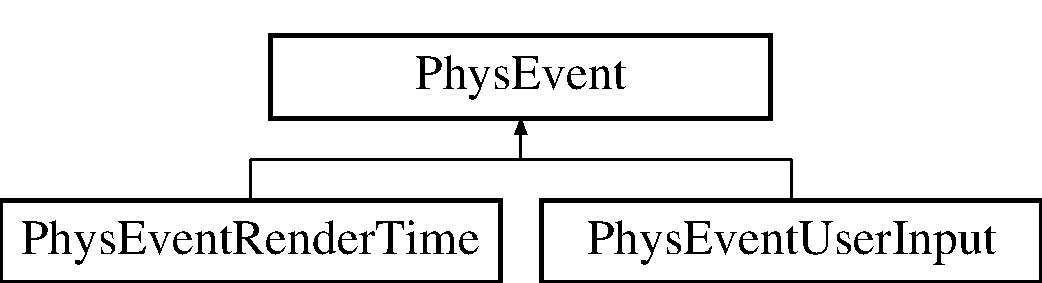
\includegraphics[height=2cm]{d9/dc2/classPhysEvent}
\end{center}
\end{figure}
\subsection*{Public Member Functions}
\begin{DoxyCompactItemize}
\item 
\hypertarget{classPhysEvent_afe21254180cdc4f12913bedcb81b6c6e}{
virtual EventType {\bfseries getEventType} ()=0}
\label{d9/dc2/classPhysEvent_afe21254180cdc4f12913bedcb81b6c6e}

\end{DoxyCompactItemize}


\subsection{Detailed Description}


Definition at line 21 of file physevent.h.

The documentation for this class was generated from the following file:\begin{DoxyCompactItemize}
\item 
physevent.h\end{DoxyCompactItemize}

\hypertarget{classPhysEventManager}{
\section{PhysEventManager Class Reference}
\label{d5/dd7/classPhysEventManager}\index{PhysEventManager@{PhysEventManager}}
}


This is a container for Events and facilitates the transfer of data.  


{\ttfamily \#include $<$physeventmanager.h$>$}\subsection*{Public Member Functions}
\begin{DoxyCompactItemize}
\item 
\hyperlink{classPhysEventManager_a1355f36d99de303cec6f3b27cadaa9ff}{PhysEventManager} (\hyperlink{classPhysWorld}{PhysWorld} $\ast$ParentWorld\_\-)
\begin{DoxyCompactList}\small\item\em Default constructor. \item\end{DoxyCompactList}\item 
unsigned int \hyperlink{classPhysEventManager_ab14d238e7abe9919be8e2d9eef388b64}{GetRemainingEventCount} ()
\begin{DoxyCompactList}\small\item\em Gets a count of events. \item\end{DoxyCompactList}\item 
\hyperlink{classPhysEvent}{PhysEvent} $\ast$ \hyperlink{classPhysEventManager_a6de94bc6c23dcbd7e15785cadee2e80b}{GetNextEvent} ()
\begin{DoxyCompactList}\small\item\em Return a pointer to the Next event. \item\end{DoxyCompactList}\item 
\hyperlink{classPhysEvent}{PhysEvent} $\ast$ \hyperlink{classPhysEventManager_a3122b32172326ac32cfecc828b820977}{PopNextEvent} ()
\begin{DoxyCompactList}\small\item\em Return a pointer to the Next event, and removes the Event from storage. \item\end{DoxyCompactList}\item 
void \hyperlink{classPhysEventManager_ad040054bd9018ff0fd27ad78ec1e87fa}{RemoveNextEvent} ()
\begin{DoxyCompactList}\small\item\em Removes an Event From the que without looking at it. \item\end{DoxyCompactList}\item 
void \hyperlink{classPhysEventManager_a7c9bb46b17f6d9245817a402dc6a2f6f}{AddEvent} (\hyperlink{classPhysEvent}{PhysEvent} $\ast$EventToAdd)
\begin{DoxyCompactList}\small\item\em Adds an event of any kind to the end of the Event Queue. \item\end{DoxyCompactList}\item 
\hypertarget{classPhysEventManager_a34b4b8d35fee0f593fbb32b83843abba}{
void {\bfseries UpdateEvents} ()}
\label{d5/dd7/classPhysEventManager_a34b4b8d35fee0f593fbb32b83843abba}

\item 
\hypertarget{classPhysEventManager_adcdeb687464f00252e1c4052d4b9304e}{
void {\bfseries UpdateSystemEvents} ()}
\label{d5/dd7/classPhysEventManager_adcdeb687464f00252e1c4052d4b9304e}

\item 
\hypertarget{classPhysEventManager_a99f2350628caf751e156107d57646030}{
void {\bfseries UpdateUserInputEvents} ()}
\label{d5/dd7/classPhysEventManager_a99f2350628caf751e156107d57646030}

\item 
\hyperlink{classPhysEventRenderTime}{PhysEventRenderTime} $\ast$ \hyperlink{classPhysEventManager_a1f2d0506ce816176913e5bdfaa9fd724}{GetNextRenderTimeEvent} ()
\begin{DoxyCompactList}\small\item\em Returns a pointer to the Next Rendertime event. \item\end{DoxyCompactList}\item 
\hyperlink{classPhysEventRenderTime}{PhysEventRenderTime} $\ast$ \hyperlink{classPhysEventManager_ad627925363fdbcff98e0faef204e81e2}{PopNextRenderTimeEvent} ()
\begin{DoxyCompactList}\small\item\em Returns a pointer to the Next Rendertime event and removes it from the Que. \item\end{DoxyCompactList}\item 
void \hyperlink{classPhysEventManager_a56acc075e743921e27284c023b3298ce}{RemoveNextRenderTimeEvent} ()
\begin{DoxyCompactList}\small\item\em Removes the First Rendertime Event From the que without looking at it. \item\end{DoxyCompactList}\item 
\hyperlink{classPhysEventUserInput}{PhysEventUserInput} $\ast$ \hyperlink{classPhysEventManager_a4874a9b1138d2351bf28e527a66c02b8}{GetNextUserInputEvent} ()
\begin{DoxyCompactList}\small\item\em Returns a pointer to the Next User Input event. \item\end{DoxyCompactList}\item 
\hyperlink{classPhysEventUserInput}{PhysEventUserInput} $\ast$ \hyperlink{classPhysEventManager_ad6612a6e1c728941e2c467e7f136ca51}{PopNextUserInputEvent} ()
\begin{DoxyCompactList}\small\item\em Returns a pointer to the Next User Input event and removes it from the Que. \item\end{DoxyCompactList}\item 
void \hyperlink{classPhysEventManager_a9c6f5296c9961fa469ebe06d7599283a}{RemoveNextUserInputEvent} ()
\begin{DoxyCompactList}\small\item\em Removes the First User Input Event From the que without looking at it. \item\end{DoxyCompactList}\item 
\hypertarget{classPhysEventManager_a61aa2ee266536d45fec2be0487f77940}{
\hyperlink{classEventQuit}{EventQuit} $\ast$ {\bfseries GetNextQuitEvent} ()}
\label{d5/dd7/classPhysEventManager_a61aa2ee266536d45fec2be0487f77940}

\item 
\hypertarget{classPhysEventManager_a1def6dcacc5dd8a0d55dd2d47fe89a1c}{
\hyperlink{classEventQuit}{EventQuit} $\ast$ {\bfseries PopNextQuitEvent} ()}
\label{d5/dd7/classPhysEventManager_a1def6dcacc5dd8a0d55dd2d47fe89a1c}

\item 
\hypertarget{classPhysEventManager_accdd3b4047b05b721f77ca68e016baf5}{
void {\bfseries RemoveNextQuitEvent} ()}
\label{d5/dd7/classPhysEventManager_accdd3b4047b05b721f77ca68e016baf5}

\item 
\hyperlink{classPhysEvent}{PhysEvent} $\ast$ \hyperlink{classPhysEventManager_a56e45572c2fb84131f7d55c060c7ac21}{GetNextSpecificEvent} (PhysEvent::EventType SpecificType)
\begin{DoxyCompactList}\small\item\em Returns a pointer to the Next kind event of the Specified type. \item\end{DoxyCompactList}\item 
\hyperlink{classPhysEvent}{PhysEvent} $\ast$ \hyperlink{classPhysEventManager_abce156f7ad7ab145b8b05740b48e6073}{PopNextSpecificEvent} (PhysEvent::EventType SpecificType)
\begin{DoxyCompactList}\small\item\em Returns a pointer to the Next kind event of the Specified type, and removes it from the Que. \item\end{DoxyCompactList}\item 
void \hyperlink{classPhysEventManager_a2d0c21e369d16cd2de97eb4c69003323}{RemoveNextSpecificEvent} (PhysEvent::EventType SpecificType)
\begin{DoxyCompactList}\small\item\em Returns a pointer to the Next kind event of the Specified type, and removes it from the Que. \item\end{DoxyCompactList}\item 
void \hyperlink{classPhysEventManager_a1e99385441c5377a741561db581ef3ae}{AddPollingCheck} (const \hyperlink{classMetaCode}{MetaCode} \&InputToTryPolling)
\begin{DoxyCompactList}\small\item\em Generates extra events each iteration of the main loop, based on user input polling. \item\end{DoxyCompactList}\item 
void \hyperlink{classPhysEventManager_af81bf9a5f081f44a6cd91fdd19d4a42a}{RemovePollingCheck} (const \hyperlink{classMetaCode}{MetaCode} \&InputToStopPolling)
\begin{DoxyCompactList}\small\item\em Removes Events from the list(s) of what needs to be polled. \item\end{DoxyCompactList}\item 
\hyperlink{classPhysEventUserInput}{PhysEventUserInput} $\ast$ \hyperlink{classPhysEventManager_ac66ebe495e2a77d06803291711528db2}{PollForUserInputEvents} ()
\begin{DoxyCompactList}\small\item\em This activates the polling routines of the user input subsystems. \item\end{DoxyCompactList}\end{DoxyCompactItemize}


\subsection{Detailed Description}
This is a container for Events and facilitates the transfer of data. The Event Manager Exists to passed important information about Gamestate from where it is generated to where it is needed. It is the Game Developers option whether they want to grab events directly using the get functions that have filters, or if they want to get all the events at once from a central location and dispatch form there. \par
 Since all User input comes in the form of events, this is also where user input Polling and optional input sources like Joysticks are controlled from. \par
 All of these event are stored in an internal Queue and order is preserved. So the First item In will be the First Out (FIFO). This is not strictly a FIFO buffer, there are a number of functions for getting of managing specific kinds of events. Generally these 'Filtered' management functions Still return the first of those kinds of event. \begin{DoxyWarning}{Warning}
Delete pointers you get from this. Anything can create events and Put them here, and anything can get them out, This means the simple way to not cause memory leaks is to have the routines extracting the events delete the events. 

Currently this is not thread safe, even though it should be. 
\end{DoxyWarning}


Definition at line 83 of file physeventmanager.h.

\subsection{Constructor \& Destructor Documentation}
\hypertarget{classPhysEventManager_a1355f36d99de303cec6f3b27cadaa9ff}{
\index{PhysEventManager@{PhysEventManager}!PhysEventManager@{PhysEventManager}}
\index{PhysEventManager@{PhysEventManager}!PhysEventManager@{PhysEventManager}}
\subsubsection[{PhysEventManager}]{\setlength{\rightskip}{0pt plus 5cm}PhysEventManager::PhysEventManager ({\bf PhysWorld} $\ast$ {\em ParentWorld\_\-})}}
\label{d5/dd7/classPhysEventManager_a1355f36d99de303cec6f3b27cadaa9ff}


Default constructor. \begin{Desc}
\item[\hyperlink{todo__todo000006}{Todo}]TODO build a deconstructor that deletes all the events still int the queue \end{Desc}

\begin{DoxyParams}{Parameters}
\item[{\em ParentWorld\_\-}]A pointer to the world that this physworld is working with Primarily\end{DoxyParams}
This creates an empty PhysEventManger

\begin{Desc}
\item[\hyperlink{todo__todo000005}{Todo}]TODO: Make the \hyperlink{classPhysEventManager}{PhysEventManager} completely thread safe. IF this is completely thread safe, we can spawn numerous individual thread each accessing this and and the performance gain would almost scale directly with cpu core count increases. Look at boost scoped\_\-lock \end{Desc}


Definition at line 89 of file physeventmanager.cpp.

\subsection{Member Function Documentation}
\hypertarget{classPhysEventManager_a7c9bb46b17f6d9245817a402dc6a2f6f}{
\index{PhysEventManager@{PhysEventManager}!AddEvent@{AddEvent}}
\index{AddEvent@{AddEvent}!PhysEventManager@{PhysEventManager}}
\subsubsection[{AddEvent}]{\setlength{\rightskip}{0pt plus 5cm}void PhysEventManager::AddEvent ({\bf PhysEvent} $\ast$ {\em EventToAdd})}}
\label{d5/dd7/classPhysEventManager_a7c9bb46b17f6d9245817a402dc6a2f6f}


Adds an event of any kind to the end of the Event Queue. 
\begin{DoxyParams}{Parameters}
\item[{\em EventToAdd}]This is a pointer to an Event.\end{DoxyParams}
This adds the existing event to the Queue. Be careful this is not delete, and does not go out of scope. Deleting the Event is now the responsibilty of the code that pulls it out of Event Manager. 

Definition at line 130 of file physeventmanager.cpp.\hypertarget{classPhysEventManager_a1e99385441c5377a741561db581ef3ae}{
\index{PhysEventManager@{PhysEventManager}!AddPollingCheck@{AddPollingCheck}}
\index{AddPollingCheck@{AddPollingCheck}!PhysEventManager@{PhysEventManager}}
\subsubsection[{AddPollingCheck}]{\setlength{\rightskip}{0pt plus 5cm}void PhysEventManager::AddPollingCheck (const {\bf MetaCode} \& {\em InputToTryPolling})}}
\label{d5/dd7/classPhysEventManager_a1e99385441c5377a741561db581ef3ae}


Generates extra events each iteration of the main loop, based on user input polling. 
\begin{DoxyParams}{Parameters}
\item[{\em InputToTryPolling}]This accepts a \hyperlink{classMetaCode}{MetaCode} and will try to watch for occurences like this one\end{DoxyParams}
This will trigger the input system to generate an event (or add to an exiting event) when polling for the given kind of event. Each Iteration of the main loop there will be a \hyperlink{classPhysEventUserInput}{PhysEventUserInput} that created. That Event will Include all the normal metacodes for user input that happened, and it will also have a meta code for each time this function was called. The added metacode may be partialky ignored, the Metavalue is almost always ignored, and in a situation where the can only be one of a given input on a system, the ID is ignore and 0 is assumed. 
\begin{DoxyExceptions}{Exceptions}
\item[{\em Unsupported Polling Check on this Platform}]When the metacode passed cannot be polled on this platform \end{DoxyExceptions}


Definition at line 283 of file physeventmanager.cpp.\hypertarget{classPhysEventManager_a6de94bc6c23dcbd7e15785cadee2e80b}{
\index{PhysEventManager@{PhysEventManager}!GetNextEvent@{GetNextEvent}}
\index{GetNextEvent@{GetNextEvent}!PhysEventManager@{PhysEventManager}}
\subsubsection[{GetNextEvent}]{\setlength{\rightskip}{0pt plus 5cm}{\bf PhysEvent} $\ast$ PhysEventManager::GetNextEvent ()}}
\label{d5/dd7/classPhysEventManager_a6de94bc6c23dcbd7e15785cadee2e80b}


Return a pointer to the Next event. This returns a pointer to the next \hyperlink{classPhysEvent}{PhysEvent}. It is advisable to use this for performance reasons because it runs in constant time. However it does not return a specific kind of event, and must be cast in order to use the true content. This returns a pointer to 0 if there are no events in the que. \begin{DoxyReturn}{Returns}
A pointer to a \hyperlink{classPhysEvent}{PhysEvent}, that still needs to be removed from the event manager and deleted. 
\end{DoxyReturn}


Definition at line 104 of file physeventmanager.cpp.\hypertarget{classPhysEventManager_a1f2d0506ce816176913e5bdfaa9fd724}{
\index{PhysEventManager@{PhysEventManager}!GetNextRenderTimeEvent@{GetNextRenderTimeEvent}}
\index{GetNextRenderTimeEvent@{GetNextRenderTimeEvent}!PhysEventManager@{PhysEventManager}}
\subsubsection[{GetNextRenderTimeEvent}]{\setlength{\rightskip}{0pt plus 5cm}{\bf PhysEventRenderTime} $\ast$ PhysEventManager::GetNextRenderTimeEvent ()}}
\label{d5/dd7/classPhysEventManager_a1f2d0506ce816176913e5bdfaa9fd724}


Returns a pointer to the Next Rendertime event. This Filtered event management function returns a pointer to the next Rendertime event. It is inadvisable to use this for performance reasons becuase it runs in linear time relative to the amount of events. However, it will return an immediately usable pointer for case where an extreme level of performance is not required. This returns a pointer to 0 if there are no rendertime events in the que. \begin{DoxyReturn}{Returns}
A pointer to a \hyperlink{classPhysEventRenderTime}{PhysEventRenderTime}, that still needs to be removed from the event manager and deleted. 
\end{DoxyReturn}


Definition at line 226 of file physeventmanager.cpp.\hypertarget{classPhysEventManager_a56e45572c2fb84131f7d55c060c7ac21}{
\index{PhysEventManager@{PhysEventManager}!GetNextSpecificEvent@{GetNextSpecificEvent}}
\index{GetNextSpecificEvent@{GetNextSpecificEvent}!PhysEventManager@{PhysEventManager}}
\subsubsection[{GetNextSpecificEvent}]{\setlength{\rightskip}{0pt plus 5cm}{\bf PhysEvent} $\ast$ PhysEventManager::GetNextSpecificEvent (PhysEvent::EventType {\em SpecificType})}}
\label{d5/dd7/classPhysEventManager_a56e45572c2fb84131f7d55c060c7ac21}


Returns a pointer to the Next kind event of the Specified type. 
\begin{DoxyParams}{Parameters}
\item[{\em SpecificType}]This is a PhysEvent::EventType that defines the type you want this to work with\end{DoxyParams}
This and the other NextSpecificEvent functions are the core of the Event Filtering System. In general the other filtering functions call one of these and does very little work on their own. \par
 This performs a linear search starting with the oldest (first entered Events) and simply checks if it the of the correct type. Then this returns a pointer to the next event of the specified type, or returns a pointer to 0 if there are none of the correct pointers in the Que. It is inadvisable to use this for performance reasons becuase it runs in linear time relative to the amount of events. \begin{DoxyReturn}{Returns}
A pointer to a \hyperlink{classPhysEventUserInput}{PhysEventUserInput}, that still needs to be removed from the event manager and deleted. 
\end{DoxyReturn}


Definition at line 183 of file physeventmanager.cpp.\hypertarget{classPhysEventManager_a4874a9b1138d2351bf28e527a66c02b8}{
\index{PhysEventManager@{PhysEventManager}!GetNextUserInputEvent@{GetNextUserInputEvent}}
\index{GetNextUserInputEvent@{GetNextUserInputEvent}!PhysEventManager@{PhysEventManager}}
\subsubsection[{GetNextUserInputEvent}]{\setlength{\rightskip}{0pt plus 5cm}{\bf PhysEventUserInput} $\ast$ PhysEventManager::GetNextUserInputEvent ()}}
\label{d5/dd7/classPhysEventManager_a4874a9b1138d2351bf28e527a66c02b8}


Returns a pointer to the Next User Input event. This Filtered event management function returns a pointer to the next User Input event. It is inadvisable to use this for performance reasons becuase it runs in linear time relative to the amount of events. However, it will return an immediately usable pointer for case where an extreme level of performance is not required. This returns a pointer to 0 if there are no User Input events in the que. \begin{DoxyReturn}{Returns}
A pointer to a \hyperlink{classPhysEventUserInput}{PhysEventUserInput}, that still needs to be removed from the event manager and deleted. 
\end{DoxyReturn}


Definition at line 245 of file physeventmanager.cpp.\hypertarget{classPhysEventManager_ab14d238e7abe9919be8e2d9eef388b64}{
\index{PhysEventManager@{PhysEventManager}!GetRemainingEventCount@{GetRemainingEventCount}}
\index{GetRemainingEventCount@{GetRemainingEventCount}!PhysEventManager@{PhysEventManager}}
\subsubsection[{GetRemainingEventCount}]{\setlength{\rightskip}{0pt plus 5cm}unsigned int PhysEventManager::GetRemainingEventCount ()}}
\label{d5/dd7/classPhysEventManager_ab14d238e7abe9919be8e2d9eef388b64}


Gets a count of events. This returns a total count of all events stored in this \hyperlink{classPhysEventManager}{PhysEventManager}. \begin{DoxyReturn}{Returns}
This returns an unsigned integer with the amount of of total events 
\end{DoxyReturn}


Definition at line 99 of file physeventmanager.cpp.\hypertarget{classPhysEventManager_ac66ebe495e2a77d06803291711528db2}{
\index{PhysEventManager@{PhysEventManager}!PollForUserInputEvents@{PollForUserInputEvents}}
\index{PollForUserInputEvents@{PollForUserInputEvents}!PhysEventManager@{PhysEventManager}}
\subsubsection[{PollForUserInputEvents}]{\setlength{\rightskip}{0pt plus 5cm}{\bf PhysEventUserInput} $\ast$ PhysEventManager::PollForUserInputEvents ()}}
\label{d5/dd7/classPhysEventManager_ac66ebe495e2a77d06803291711528db2}


This activates the polling routines of the user input subsystems. This checks the current state of user input devices that have been added by \hyperlink{classPhysEventManager_a1e99385441c5377a741561db581ef3ae}{AddPollingCheck(const MetaCode \&InputToTryPolling)}. This is called automatically by main loop processing, but there is no harm in calling it several times. \begin{DoxyReturn}{Returns}
This returns a pointer to a \hyperlink{classPhysEventUserInput}{PhysEventUserInput} that contains the desired metacodes 
\end{DoxyReturn}


Definition at line 323 of file physeventmanager.cpp.\hypertarget{classPhysEventManager_a3122b32172326ac32cfecc828b820977}{
\index{PhysEventManager@{PhysEventManager}!PopNextEvent@{PopNextEvent}}
\index{PopNextEvent@{PopNextEvent}!PhysEventManager@{PhysEventManager}}
\subsubsection[{PopNextEvent}]{\setlength{\rightskip}{0pt plus 5cm}{\bf PhysEvent} $\ast$ PhysEventManager::PopNextEvent ()}}
\label{d5/dd7/classPhysEventManager_a3122b32172326ac32cfecc828b820977}


Return a pointer to the Next event, and removes the Event from storage. This functions just like GetNextEvent , except that it also removes the item from the internal storage of the \hyperlink{classPhysEventManager}{PhysEventManager}. This returns a pointer to 0 if there are no events in the que. \begin{DoxyReturn}{Returns}
A pointer to a \hyperlink{classPhysEvent}{PhysEvent}, that will need to be deleted once it has been used. 
\end{DoxyReturn}


Definition at line 114 of file physeventmanager.cpp.\hypertarget{classPhysEventManager_ad627925363fdbcff98e0faef204e81e2}{
\index{PhysEventManager@{PhysEventManager}!PopNextRenderTimeEvent@{PopNextRenderTimeEvent}}
\index{PopNextRenderTimeEvent@{PopNextRenderTimeEvent}!PhysEventManager@{PhysEventManager}}
\subsubsection[{PopNextRenderTimeEvent}]{\setlength{\rightskip}{0pt plus 5cm}{\bf PhysEventRenderTime} $\ast$ PhysEventManager::PopNextRenderTimeEvent ()}}
\label{d5/dd7/classPhysEventManager_ad627925363fdbcff98e0faef204e81e2}


Returns a pointer to the Next Rendertime event and removes it from the Que. This Filtered event management function returns a pointer to the next Rendertime event. It is inadvisable to use this for performance reasons becuase it runs in linear time relative to the amount of events. However, it will return an immediately usable pointer for case where an extreme level of performance is not required. This returns a pointer to 0 if there are no rendertime events in the que. This also removes the returned pointer form the Que. \begin{DoxyReturn}{Returns}
A pointer to a \hyperlink{classPhysEventRenderTime}{PhysEventRenderTime}, that still needs to be removed from the event manager and deleted. 
\end{DoxyReturn}


Definition at line 231 of file physeventmanager.cpp.\hypertarget{classPhysEventManager_abce156f7ad7ab145b8b05740b48e6073}{
\index{PhysEventManager@{PhysEventManager}!PopNextSpecificEvent@{PopNextSpecificEvent}}
\index{PopNextSpecificEvent@{PopNextSpecificEvent}!PhysEventManager@{PhysEventManager}}
\subsubsection[{PopNextSpecificEvent}]{\setlength{\rightskip}{0pt plus 5cm}{\bf PhysEvent} $\ast$ PhysEventManager::PopNextSpecificEvent (PhysEvent::EventType {\em SpecificType})}}
\label{d5/dd7/classPhysEventManager_abce156f7ad7ab145b8b05740b48e6073}


Returns a pointer to the Next kind event of the Specified type, and removes it from the Que. 
\begin{DoxyParams}{Parameters}
\item[{\em SpecificType}]This is a PhysEvent::EventType that defines the type you want this to work with\end{DoxyParams}
This is just like \hyperlink{classPhysEventManager_a56e45572c2fb84131f7d55c060c7ac21}{GetNextSpecificEvent(PhysEvent::EventType SpecificType)} but it also removes the item from the Que. \begin{DoxyReturn}{Returns}
A pointer to a \hyperlink{classPhysEventUserInput}{PhysEventUserInput}, that still needs to be removed from the event manager and deleted. 
\end{DoxyReturn}


Definition at line 197 of file physeventmanager.cpp.\hypertarget{classPhysEventManager_ad6612a6e1c728941e2c467e7f136ca51}{
\index{PhysEventManager@{PhysEventManager}!PopNextUserInputEvent@{PopNextUserInputEvent}}
\index{PopNextUserInputEvent@{PopNextUserInputEvent}!PhysEventManager@{PhysEventManager}}
\subsubsection[{PopNextUserInputEvent}]{\setlength{\rightskip}{0pt plus 5cm}{\bf PhysEventUserInput} $\ast$ PhysEventManager::PopNextUserInputEvent ()}}
\label{d5/dd7/classPhysEventManager_ad6612a6e1c728941e2c467e7f136ca51}


Returns a pointer to the Next User Input event and removes it from the Que. This Filtered event management function returns a pointer to the next User Input event. It is inadvisable to use this for performance reasons becuase it runs in linear time relative to the amount of events. However, it will return an immediately usable pointer for case where an extreme level of performance is not required. This returns a pointer to 0 if there are no User Input events in the que. This also removes the returned pointer form the Que. \begin{DoxyReturn}{Returns}
A pointer to a \hyperlink{classPhysEventUserInput}{PhysEventUserInput}, that still needs to be removed from the event manager and deleted. 
\end{DoxyReturn}


Definition at line 250 of file physeventmanager.cpp.\hypertarget{classPhysEventManager_ad040054bd9018ff0fd27ad78ec1e87fa}{
\index{PhysEventManager@{PhysEventManager}!RemoveNextEvent@{RemoveNextEvent}}
\index{RemoveNextEvent@{RemoveNextEvent}!PhysEventManager@{PhysEventManager}}
\subsubsection[{RemoveNextEvent}]{\setlength{\rightskip}{0pt plus 5cm}void PhysEventManager::RemoveNextEvent ()}}
\label{d5/dd7/classPhysEventManager_ad040054bd9018ff0fd27ad78ec1e87fa}


Removes an Event From the que without looking at it. This together with \hyperlink{classPhysEventManager_a6de94bc6c23dcbd7e15785cadee2e80b}{GetNextEvent()} are the same as call \hyperlink{classPhysEventManager_a3122b32172326ac32cfecc828b820977}{PopNextEvent()}. \begin{DoxyWarning}{Warning}
If you did not call \hyperlink{classPhysEventManager_a6de94bc6c23dcbd7e15785cadee2e80b}{GetNextEvent()} and haven't deleted or stored, or somehow dealt with this pointer, then this is a memory leak. Don't use this unless you are certain you have taken care of the pointer appropriately 
\end{DoxyWarning}

\begin{DoxyExceptions}{Exceptions}
\item[{\em This}]can throw any STL exception a que could. Any with likely throw some kind of except if called when there are no Events in the Que. \end{DoxyExceptions}


Definition at line 125 of file physeventmanager.cpp.\hypertarget{classPhysEventManager_a56acc075e743921e27284c023b3298ce}{
\index{PhysEventManager@{PhysEventManager}!RemoveNextRenderTimeEvent@{RemoveNextRenderTimeEvent}}
\index{RemoveNextRenderTimeEvent@{RemoveNextRenderTimeEvent}!PhysEventManager@{PhysEventManager}}
\subsubsection[{RemoveNextRenderTimeEvent}]{\setlength{\rightskip}{0pt plus 5cm}void PhysEventManager::RemoveNextRenderTimeEvent ()}}
\label{d5/dd7/classPhysEventManager_a56acc075e743921e27284c023b3298ce}


Removes the First Rendertime Event From the que without looking at it. This together with \hyperlink{classPhysEventManager_a1f2d0506ce816176913e5bdfaa9fd724}{GetNextRenderTimeEvent()} are the pretty much same as call \hyperlink{classPhysEventManager_ad627925363fdbcff98e0faef204e81e2}{PopNextRenderTimeEvent()}. \begin{DoxyWarning}{Warning}
If you did not call \hyperlink{classPhysEventManager_a1f2d0506ce816176913e5bdfaa9fd724}{GetNextRenderTimeEvent()} and haven't deleted or stored, or somehow dealt with this pointer, then this is a memory leak. Don't use this unless you are certain you have taken care of the pointer appropriately 
\end{DoxyWarning}

\begin{DoxyExceptions}{Exceptions}
\item[{\em This}]can throw any STL exception a queue could. And with likely throw some kind of except if called when there are no Events in the Que. \end{DoxyExceptions}


Definition at line 236 of file physeventmanager.cpp.\hypertarget{classPhysEventManager_a2d0c21e369d16cd2de97eb4c69003323}{
\index{PhysEventManager@{PhysEventManager}!RemoveNextSpecificEvent@{RemoveNextSpecificEvent}}
\index{RemoveNextSpecificEvent@{RemoveNextSpecificEvent}!PhysEventManager@{PhysEventManager}}
\subsubsection[{RemoveNextSpecificEvent}]{\setlength{\rightskip}{0pt plus 5cm}void PhysEventManager::RemoveNextSpecificEvent (PhysEvent::EventType {\em SpecificType})}}
\label{d5/dd7/classPhysEventManager_a2d0c21e369d16cd2de97eb4c69003323}


Returns a pointer to the Next kind event of the Specified type, and removes it from the Que. 
\begin{DoxyParams}{Parameters}
\item[{\em SpecificType}]This is a PhysEvent::EventType that defines the type you want this to work with\end{DoxyParams}
This is just like \hyperlink{classPhysEventManager_abce156f7ad7ab145b8b05740b48e6073}{PopNextSpecificEvent(PhysEvent::EventType SpecificType)} but exept it doesn't bother with any of the needed structure involved with returning data, and just removes the specific evetn from the Que. \begin{DoxyWarning}{Warning}
If you did not call \hyperlink{classPhysEventManager_a56e45572c2fb84131f7d55c060c7ac21}{GetNextSpecificEvent(PhysEvent::EventType SpecificType)} and haven't deleted or stored, or somehow dealt with this pointer, then this is a memory leak. Don't use this unless you are certain you have taken care of the pointer appropriately. 
\end{DoxyWarning}

\begin{DoxyExceptions}{Exceptions}
\item[{\em This}]can throw any STL exception a queue could. And with likely throw some kind of except if called when there are no Events in the Que. \end{DoxyExceptions}


Definition at line 212 of file physeventmanager.cpp.\hypertarget{classPhysEventManager_a9c6f5296c9961fa469ebe06d7599283a}{
\index{PhysEventManager@{PhysEventManager}!RemoveNextUserInputEvent@{RemoveNextUserInputEvent}}
\index{RemoveNextUserInputEvent@{RemoveNextUserInputEvent}!PhysEventManager@{PhysEventManager}}
\subsubsection[{RemoveNextUserInputEvent}]{\setlength{\rightskip}{0pt plus 5cm}void PhysEventManager::RemoveNextUserInputEvent ()}}
\label{d5/dd7/classPhysEventManager_a9c6f5296c9961fa469ebe06d7599283a}


Removes the First User Input Event From the que without looking at it. This together with \hyperlink{classPhysEventManager_a4874a9b1138d2351bf28e527a66c02b8}{GetNextUserInputEvent()} are the pretty much same as call \hyperlink{classPhysEventManager_ad6612a6e1c728941e2c467e7f136ca51}{PopNextUserInputEvent()}. \begin{DoxyWarning}{Warning}
If you did not call \hyperlink{classPhysEventManager_a4874a9b1138d2351bf28e527a66c02b8}{GetNextUserInputEvent()} and haven't deleted or stored, or somehow dealt with this pointer, then this is a memory leak. Don't use this unless you are certain you have taken care of the pointer appropriately 
\end{DoxyWarning}

\begin{DoxyExceptions}{Exceptions}
\item[{\em This}]can throw any STL exception a queue could. And with likely throw some kind of except if called when there are no Events in the Que. \end{DoxyExceptions}


Definition at line 255 of file physeventmanager.cpp.\hypertarget{classPhysEventManager_af81bf9a5f081f44a6cd91fdd19d4a42a}{
\index{PhysEventManager@{PhysEventManager}!RemovePollingCheck@{RemovePollingCheck}}
\index{RemovePollingCheck@{RemovePollingCheck}!PhysEventManager@{PhysEventManager}}
\subsubsection[{RemovePollingCheck}]{\setlength{\rightskip}{0pt plus 5cm}void PhysEventManager::RemovePollingCheck (const {\bf MetaCode} \& {\em InputToStopPolling})}}
\label{d5/dd7/classPhysEventManager_af81bf9a5f081f44a6cd91fdd19d4a42a}


Removes Events from the list(s) of what needs to be polled. 
\begin{DoxyParams}{Parameters}
\item[{\em InputToStopPolling}]This accepts a \hyperlink{classMetaCode}{MetaCode} and will try to Remove Watches like this one\end{DoxyParams}
This will remove any check for polling that share the same inputcode and ID. This 
\begin{DoxyExceptions}{Exceptions}
\item[{\em Polling check not present}]Is thrown \end{DoxyExceptions}


The documentation for this class was generated from the following files:\begin{DoxyCompactItemize}
\item 
physeventmanager.h\item 
physeventmanager.cpp\end{DoxyCompactItemize}

\hypertarget{classPhysEventRenderTime}{
\section{PhysEventRenderTime Class Reference}
\label{d4/d83/classPhysEventRenderTime}\index{PhysEventRenderTime@{PhysEventRenderTime}}
}
Inheritance diagram for PhysEventRenderTime::\begin{figure}[H]
\begin{center}
\leavevmode
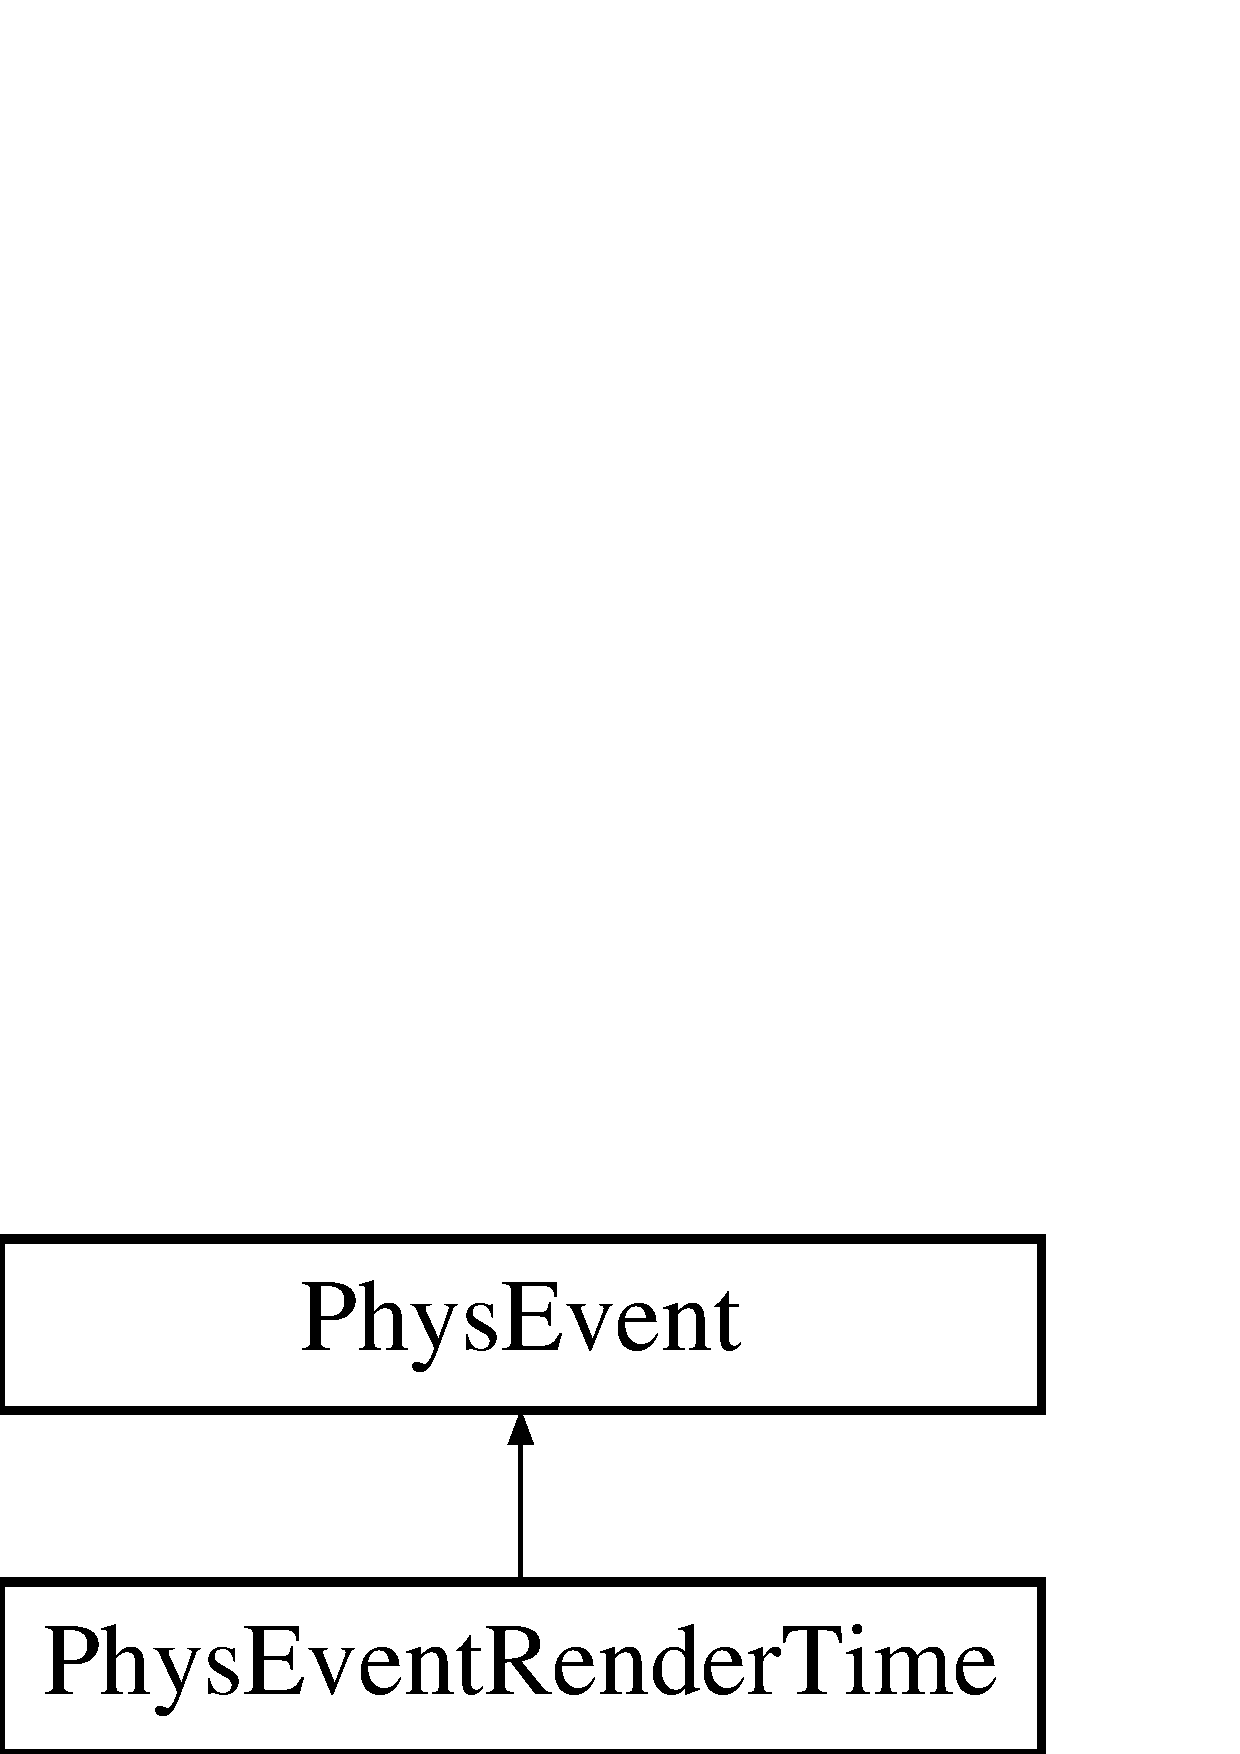
\includegraphics[height=2cm]{d4/d83/classPhysEventRenderTime}
\end{center}
\end{figure}
\subsection*{Public Member Functions}
\begin{DoxyCompactItemize}
\item 
\hypertarget{classPhysEventRenderTime_af6ad859225b0c869af9145844ac5a248}{
{\bfseries PhysEventRenderTime} (PhysWhole Milliseconds)}
\label{d4/d83/classPhysEventRenderTime_af6ad859225b0c869af9145844ac5a248}

\item 
virtual \hyperlink{classphys_1_1Event_af5fdbb3e08d8e578d58770fbc606fda7}{EventType} \hyperlink{classPhysEventRenderTime_a96b0569f8b1cd459383318c9437130d4}{getEventType} () const 
\begin{DoxyCompactList}\small\item\em This will aid in identifying all classes that inherit from this class. \item\end{DoxyCompactList}\item 
\hypertarget{classPhysEventRenderTime_aaba6aa77d58877dc8b3784c1ebcfe7b6}{
PhysWhole {\bfseries getMilliSecondsSinceLastFrame} ()}
\label{d4/d83/classPhysEventRenderTime_aaba6aa77d58877dc8b3784c1ebcfe7b6}

\end{DoxyCompactItemize}


\subsection{Detailed Description}


Definition at line 53 of file physeventrendertime.h.

\subsection{Member Function Documentation}
\hypertarget{classPhysEventRenderTime_a96b0569f8b1cd459383318c9437130d4}{
\index{PhysEventRenderTime@{PhysEventRenderTime}!getEventType@{getEventType}}
\index{getEventType@{getEventType}!PhysEventRenderTime@{PhysEventRenderTime}}
\subsubsection[{getEventType}]{\setlength{\rightskip}{0pt plus 5cm}{\bf Event::EventType} PhysEventRenderTime::getEventType () const\hspace{0.3cm}{\ttfamily  \mbox{[}virtual\mbox{]}}}}
\label{d4/d83/classPhysEventRenderTime_a96b0569f8b1cd459383318c9437130d4}


This will aid in identifying all classes that inherit from this class. All Classes derived form this calls will return an Event::EventType that correspond the the data/class type they actually are. \begin{DoxyReturn}{Returns}
This returns an eventype that will correspend with the actual event type. This can be used on all Phys game provided class to safely cast a pointer to the correct event type. 
\end{DoxyReturn}


Implements \hyperlink{classphys_1_1Event_ac2c0623a6bc399e62f4b9fb2c022ea73}{phys::Event}.

Definition at line 56 of file physeventrendertime.cpp.

The documentation for this class was generated from the following files:\begin{DoxyCompactItemize}
\item 
physeventrendertime.h\item 
physeventrendertime.cpp\end{DoxyCompactItemize}

\hypertarget{classPhysEventUserInput}{
\section{PhysEventUserInput Class Reference}
\label{dc/d0e/classPhysEventUserInput}\index{PhysEventUserInput@{PhysEventUserInput}}
}


This is a container for MetaCodes that is used in the physEventManager.  


{\ttfamily \#include $<$physeventuserinput.h$>$}Inheritance diagram for PhysEventUserInput::\begin{figure}[H]
\begin{center}
\leavevmode
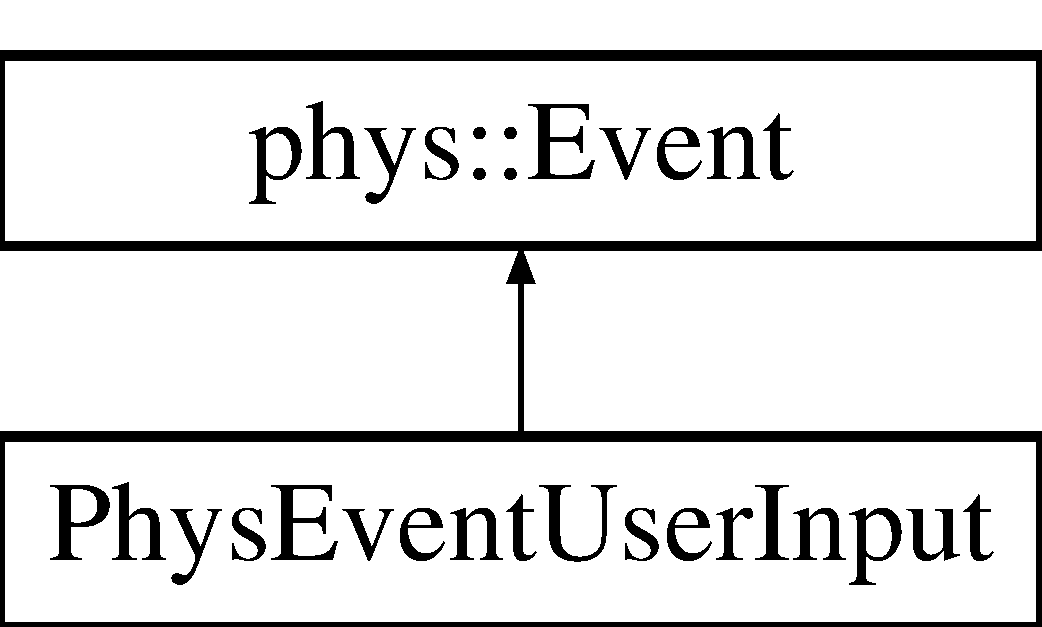
\includegraphics[height=2cm]{dc/d0e/classPhysEventUserInput}
\end{center}
\end{figure}
\subsection*{Public Member Functions}
\begin{DoxyCompactItemize}
\item 
\hyperlink{classPhysEventUserInput_a6f8eaf698e8109d5cb30f2f17044f1ba}{PhysEventUserInput} ()
\begin{DoxyCompactList}\small\item\em Default constructor. \item\end{DoxyCompactList}\item 
\hyperlink{classPhysEventUserInput_ae13b1b02bfa3ef64dc4205478a68810f}{PhysEventUserInput} (const \hyperlink{classMetaCode}{MetaCode} \&Code\_\-)
\begin{DoxyCompactList}\small\item\em Single Data Point constructor. \item\end{DoxyCompactList}\item 
\hyperlink{classPhysEventUserInput_a0a9bd99d8db6f171ef3c87bd417ccc4a}{PhysEventUserInput} (const vector$<$ \hyperlink{classMetaCode}{MetaCode} $>$ \&Codes\_\-)
\begin{DoxyCompactList}\small\item\em Multi Data Point constructor. \item\end{DoxyCompactList}\item 
const \hyperlink{classMetaCode}{MetaCode} \hyperlink{classPhysEventUserInput_aa564530c27f6983bb412e46c2c7ed086}{GetMetaCode} (const unsigned int \&Index)
\begin{DoxyCompactList}\small\item\em Single Data Point constructor. \item\end{DoxyCompactList}\item 
unsigned int \hyperlink{classPhysEventUserInput_a86df812a38566a572134100a422a8799}{GetMetaCodeCount} ()
\begin{DoxyCompactList}\small\item\em Retrieves a count of the stored Metacodes. \item\end{DoxyCompactList}\item 
void \hyperlink{classPhysEventUserInput_a4f5b94c64cd08c15b480e441d25a385d}{AddCode} (const \hyperlink{classMetaCode}{MetaCode} \&Code\_\-)
\begin{DoxyCompactList}\small\item\em Adds a \hyperlink{classMetaCode}{MetaCode}. \item\end{DoxyCompactList}\item 
void \hyperlink{classPhysEventUserInput_ace3b98a502b8e784b58bc5dc599fc0c4}{AddCode} (const int \&MetaValue\_\-, const short unsigned int \&ID\_\-, const \hyperlink{classMetaCode_a7390e6f58e25c0ce377bba4e63081b24}{MetaCode::InputCode} \&Code\_\-)
\begin{DoxyCompactList}\small\item\em Adds a Created From Raw Values. \item\end{DoxyCompactList}\item 
void \hyperlink{classPhysEventUserInput_a385a4f7a6e88be43b6ba1ffc2a1bb5e3}{AddCode} (const RawEvent \&RawEvent\_\-)
\begin{DoxyCompactList}\small\item\em Adds a \hyperlink{classMetaCode}{MetaCode} created from a RawEvent. \item\end{DoxyCompactList}\item 
void \hyperlink{classPhysEventUserInput_aecac02073d3296c71e0ae4534daf8dce}{AddCode} (const vector$<$ \hyperlink{classMetaCode}{MetaCode} $>$ \&Codes)
\begin{DoxyCompactList}\small\item\em Add Several MetaCodes from a vector. \item\end{DoxyCompactList}\item 
void \hyperlink{classPhysEventUserInput_a9e42f42f9a4a42f792e5cf95856669c0}{AddCodesFromRawEvent} (const RawEvent \&RawEvent\_\-)
\begin{DoxyCompactList}\small\item\em Adds all possible MetaCodes that can be created from the given RawEvent. \item\end{DoxyCompactList}\item 
void \hyperlink{classPhysEventUserInput_a1dbd2996770df334fba9f67d9bb4ffa0}{EraseCode} (const \hyperlink{classMetaCode}{MetaCode} \&Code\_\-)
\begin{DoxyCompactList}\small\item\em Removes a specific code from storage. \item\end{DoxyCompactList}\item 
void \hyperlink{classPhysEventUserInput_a8cbbee3c2be3bd12746ad442fce526e4}{EraseCode} (const unsigned int \&Index)
\begin{DoxyCompactList}\small\item\em Removes a specific code from storage. \item\end{DoxyCompactList}\item 
void \hyperlink{classPhysEventUserInput_a8325bb0172db6ea02fd06f4a5d1a7378}{ToggleCode} (const \hyperlink{classMetaCode}{MetaCode} \&Code\_\-)
\begin{DoxyCompactList}\small\item\em Removes a specific code or Adds it if not present. \item\end{DoxyCompactList}\item 
\hyperlink{classPhysEventUserInput}{PhysEventUserInput} \& \hyperlink{classPhysEventUserInput_a257c2e093b5736324e39d5fac0d6de2a}{operator+=} (const \hyperlink{classPhysEventUserInput}{PhysEventUserInput} \&Add)
\begin{DoxyCompactList}\small\item\em This add all of one \hyperlink{classPhysEventUserInput}{PhysEventUserInput} to another. \item\end{DoxyCompactList}\item 
virtual EventType \hyperlink{classPhysEventUserInput_ab89b06b8f7aa148cad453ca9fcae5b89}{getEventType} ()
\begin{DoxyCompactList}\small\item\em Returns the type of this event. \item\end{DoxyCompactList}\end{DoxyCompactItemize}
\subsection*{Protected Attributes}
\begin{DoxyCompactItemize}
\item 
\hypertarget{classPhysEventUserInput_a51607772d8a5b9f401ad0efc964ec129}{
vector$<$ \hyperlink{classMetaCode}{MetaCode} $>$ {\bfseries Code}}
\label{dc/d0e/classPhysEventUserInput_a51607772d8a5b9f401ad0efc964ec129}

\end{DoxyCompactItemize}


\subsection{Detailed Description}
This is a container for MetaCodes that is used in the physEventManager. The \hyperlink{classPhysEventUserInput}{PhysEventUserInput} is the container for information about how a user enters data and commands into a program. By Default one is inserted into event manager the with all the user input from the last run of the main loop. These can be manually inserted into the EventManager to simulate input from other sources. If setup properly this can allow computer controlled characters to use the same interface players, allowing for more realistic response from them. This is not limited to the tricks discussed here. 

Definition at line 93 of file physeventuserinput.h.

\subsection{Constructor \& Destructor Documentation}
\hypertarget{classPhysEventUserInput_a6f8eaf698e8109d5cb30f2f17044f1ba}{
\index{PhysEventUserInput@{PhysEventUserInput}!PhysEventUserInput@{PhysEventUserInput}}
\index{PhysEventUserInput@{PhysEventUserInput}!PhysEventUserInput@{PhysEventUserInput}}
\subsubsection[{PhysEventUserInput}]{\setlength{\rightskip}{0pt plus 5cm}PhysEventUserInput::PhysEventUserInput ()}}
\label{dc/d0e/classPhysEventUserInput_a6f8eaf698e8109d5cb30f2f17044f1ba}


Default constructor. This creates a perfectly functional, but empty \hyperlink{classPhysEventUserInput}{PhysEventUserInput}. 

Definition at line 64 of file physeventuserinput.cpp.\hypertarget{classPhysEventUserInput_ae13b1b02bfa3ef64dc4205478a68810f}{
\index{PhysEventUserInput@{PhysEventUserInput}!PhysEventUserInput@{PhysEventUserInput}}
\index{PhysEventUserInput@{PhysEventUserInput}!PhysEventUserInput@{PhysEventUserInput}}
\subsubsection[{PhysEventUserInput}]{\setlength{\rightskip}{0pt plus 5cm}PhysEventUserInput::PhysEventUserInput (const {\bf MetaCode} \& {\em Code\_\-})}}
\label{dc/d0e/classPhysEventUserInput_ae13b1b02bfa3ef64dc4205478a68810f}


Single Data Point constructor. 
\begin{DoxyParams}{Parameters}
\item[{\em Code\_\-}]This \hyperlink{classMetaCode}{MetaCode} will be added to the \hyperlink{classPhysEventUserInput}{PhysEventUserInput} during creation.\end{DoxyParams}
This creates a functional \hyperlink{classPhysEventUserInput}{PhysEventUserInput} which already contains one metacode. 

Definition at line 69 of file physeventuserinput.cpp.\hypertarget{classPhysEventUserInput_a0a9bd99d8db6f171ef3c87bd417ccc4a}{
\index{PhysEventUserInput@{PhysEventUserInput}!PhysEventUserInput@{PhysEventUserInput}}
\index{PhysEventUserInput@{PhysEventUserInput}!PhysEventUserInput@{PhysEventUserInput}}
\subsubsection[{PhysEventUserInput}]{\setlength{\rightskip}{0pt plus 5cm}PhysEventUserInput::PhysEventUserInput (const vector$<$ {\bf MetaCode} $>$ \& {\em Codes\_\-})}}
\label{dc/d0e/classPhysEventUserInput_a0a9bd99d8db6f171ef3c87bd417ccc4a}


Multi Data Point constructor. 
\begin{DoxyParams}{Parameters}
\item[{\em Code\_\-}]The MetaCodes in this vecotor will be added to the \hyperlink{classPhysEventUserInput}{PhysEventUserInput} during creation.\end{DoxyParams}
This creates a ready to use \hyperlink{classPhysEventUserInput}{PhysEventUserInput} which already contains all the metacodes included. 

Definition at line 74 of file physeventuserinput.cpp.

\subsection{Member Function Documentation}
\hypertarget{classPhysEventUserInput_aecac02073d3296c71e0ae4534daf8dce}{
\index{PhysEventUserInput@{PhysEventUserInput}!AddCode@{AddCode}}
\index{AddCode@{AddCode}!PhysEventUserInput@{PhysEventUserInput}}
\subsubsection[{AddCode}]{\setlength{\rightskip}{0pt plus 5cm}void PhysEventUserInput::AddCode (const vector$<$ {\bf MetaCode} $>$ \& {\em Codes})}}
\label{dc/d0e/classPhysEventUserInput_aecac02073d3296c71e0ae4534daf8dce}


Add Several MetaCodes from a vector. 
\begin{DoxyParams}{Parameters}
\item[{\em Codes\_\-}]A vector of MetaCodes to be added to this event\end{DoxyParams}
This adds several existing metacodes to this event. 

Definition at line 111 of file physeventuserinput.cpp.\hypertarget{classPhysEventUserInput_a385a4f7a6e88be43b6ba1ffc2a1bb5e3}{
\index{PhysEventUserInput@{PhysEventUserInput}!AddCode@{AddCode}}
\index{AddCode@{AddCode}!PhysEventUserInput@{PhysEventUserInput}}
\subsubsection[{AddCode}]{\setlength{\rightskip}{0pt plus 5cm}void PhysEventUserInput::AddCode (const RawEvent \& {\em RawEvent\_\-})}}
\label{dc/d0e/classPhysEventUserInput_a385a4f7a6e88be43b6ba1ffc2a1bb5e3}


Adds a \hyperlink{classMetaCode}{MetaCode} created from a RawEvent. 
\begin{DoxyParams}{Parameters}
\item[{\em RawEvent\_\-}]The RawEvent which will be translated into exactly One \hyperlink{classMetaCode}{MetaCode}\end{DoxyParams}
This will add \hyperlink{classMetaCode}{MetaCode} to this event which will be create from a RawEvent which can produce Exactly one \hyperlink{classMetaCode}{MetaCode}. This is used by engine internals, it is recommended to not use this in game code. \begin{DoxyWarning}{Warning}
Do not use this without reading and fully understanding the warnings on \hyperlink{classMetaCode_a87b260ce7ee3a66c75320c0fc37cdc0a}{MetaCode::MetaCode(const RawEvent \&RawEvent\_\-)} . This function has all the same Restrictions. If game code is using RawEvents at all, the game logic should be scrutinized carefully, it is probably wrong, but if it must it should use \hyperlink{classPhysEventUserInput_a9e42f42f9a4a42f792e5cf95856669c0}{PhysEventUserInput::AddCodesFromRawEvent} instead, as it can make the needed determinations automatically and in a platform agnostic way. 
\end{DoxyWarning}


Definition at line 99 of file physeventuserinput.cpp.\hypertarget{classPhysEventUserInput_ace3b98a502b8e784b58bc5dc599fc0c4}{
\index{PhysEventUserInput@{PhysEventUserInput}!AddCode@{AddCode}}
\index{AddCode@{AddCode}!PhysEventUserInput@{PhysEventUserInput}}
\subsubsection[{AddCode}]{\setlength{\rightskip}{0pt plus 5cm}void PhysEventUserInput::AddCode (const int \& {\em MetaValue\_\-}, \/  const short unsigned int \& {\em ID\_\-}, \/  const {\bf MetaCode::InputCode} \& {\em Code\_\-})}}
\label{dc/d0e/classPhysEventUserInput_ace3b98a502b8e784b58bc5dc599fc0c4}


Adds a Created From Raw Values. 
\begin{DoxyParams}{Parameters}
\item[{\em MetaValue\_\-}]The MetaValue that will be in the \hyperlink{classMetaCode}{MetaCode} \item[{\em ID\_\-}]The ID that will be in the \hyperlink{classMetaCode}{MetaCode} \item[{\em Code\_\-}]The InputCode that will be in the \hyperlink{classMetaCode}{MetaCode}\end{DoxyParams}
This creates metacode a metacode and adds it to this event. 

Definition at line 105 of file physeventuserinput.cpp.\hypertarget{classPhysEventUserInput_a4f5b94c64cd08c15b480e441d25a385d}{
\index{PhysEventUserInput@{PhysEventUserInput}!AddCode@{AddCode}}
\index{AddCode@{AddCode}!PhysEventUserInput@{PhysEventUserInput}}
\subsubsection[{AddCode}]{\setlength{\rightskip}{0pt plus 5cm}void PhysEventUserInput::AddCode (const {\bf MetaCode} \& {\em Code\_\-})}}
\label{dc/d0e/classPhysEventUserInput_a4f5b94c64cd08c15b480e441d25a385d}


Adds a \hyperlink{classMetaCode}{MetaCode}. 
\begin{DoxyParams}{Parameters}
\item[{\em Code\_\-}]The User Input \hyperlink{classMetaCode}{MetaCode} tobe added\end{DoxyParams}
This adds an existing metacode to this event. 

Definition at line 94 of file physeventuserinput.cpp.\hypertarget{classPhysEventUserInput_a9e42f42f9a4a42f792e5cf95856669c0}{
\index{PhysEventUserInput@{PhysEventUserInput}!AddCodesFromRawEvent@{AddCodesFromRawEvent}}
\index{AddCodesFromRawEvent@{AddCodesFromRawEvent}!PhysEventUserInput@{PhysEventUserInput}}
\subsubsection[{AddCodesFromRawEvent}]{\setlength{\rightskip}{0pt plus 5cm}void PhysEventUserInput::AddCodesFromRawEvent (const RawEvent \& {\em RawEvent\_\-})}}
\label{dc/d0e/classPhysEventUserInput_a9e42f42f9a4a42f792e5cf95856669c0}


Adds all possible MetaCodes that can be created from the given RawEvent. 
\begin{DoxyParams}{Parameters}
\item[{\em RawEvent\_\-}]The RawEvent which will be translated into a group of metacodes and added to this\end{DoxyParams}
This will add \hyperlink{classMetaCode}{MetaCode} to this event which will be create from a RawEvent which can produce Exactly one \hyperlink{classMetaCode}{MetaCode}. This is used by engine internals, it is recommended to not use this in game code. \begin{DoxyWarning}{Warning}
If game code is using RawEvents at all, the game logic should be scrutinized carefully, it is probably wrong, but if it must them this is the correct function to use. This will work same on a all platforms. However, the binary format of the Rawevent could chnage meaning you would have to recompile the game code to work with new version of the engine \par
 This Function is currently incomplete, and does not yet process all events such as joysticks events and some mouse events. 
\end{DoxyWarning}


Definition at line 162 of file physeventuserinput.cpp.\hypertarget{classPhysEventUserInput_a8cbbee3c2be3bd12746ad442fce526e4}{
\index{PhysEventUserInput@{PhysEventUserInput}!EraseCode@{EraseCode}}
\index{EraseCode@{EraseCode}!PhysEventUserInput@{PhysEventUserInput}}
\subsubsection[{EraseCode}]{\setlength{\rightskip}{0pt plus 5cm}void PhysEventUserInput::EraseCode (const unsigned int \& {\em Index})}}
\label{dc/d0e/classPhysEventUserInput_a8cbbee3c2be3bd12746ad442fce526e4}


Removes a specific code from storage. 
\begin{DoxyParams}{Parameters}
\item[{\em Index}]This is the location to removed from\end{DoxyParams}
The \hyperlink{classMetaCode}{MetaCode} at and only at the given Index will be deleted. 

Definition at line 133 of file physeventuserinput.cpp.\hypertarget{classPhysEventUserInput_a1dbd2996770df334fba9f67d9bb4ffa0}{
\index{PhysEventUserInput@{PhysEventUserInput}!EraseCode@{EraseCode}}
\index{EraseCode@{EraseCode}!PhysEventUserInput@{PhysEventUserInput}}
\subsubsection[{EraseCode}]{\setlength{\rightskip}{0pt plus 5cm}void PhysEventUserInput::EraseCode (const {\bf MetaCode} \& {\em Code\_\-})}}
\label{dc/d0e/classPhysEventUserInput_a1dbd2996770df334fba9f67d9bb4ffa0}


Removes a specific code from storage. 
\begin{DoxyParams}{Parameters}
\item[{\em Code\_\-}]This will search for all matching copies of this\end{DoxyParams}
All MetaCodes that are equal to Code\_\- will simply be erased. 

Definition at line 120 of file physeventuserinput.cpp.\hypertarget{classPhysEventUserInput_ab89b06b8f7aa148cad453ca9fcae5b89}{
\index{PhysEventUserInput@{PhysEventUserInput}!getEventType@{getEventType}}
\index{getEventType@{getEventType}!PhysEventUserInput@{PhysEventUserInput}}
\subsubsection[{getEventType}]{\setlength{\rightskip}{0pt plus 5cm}PhysEvent::EventType PhysEventUserInput::getEventType ()\hspace{0.3cm}{\ttfamily  \mbox{[}virtual\mbox{]}}}}
\label{dc/d0e/classPhysEventUserInput_ab89b06b8f7aa148cad453ca9fcae5b89}


Returns the type of this event. \begin{DoxyReturn}{Returns}
Returns EventType::UserInput 
\end{DoxyReturn}


Implements \hyperlink{classPhysEvent}{PhysEvent}.

Definition at line 157 of file physeventuserinput.cpp.\hypertarget{classPhysEventUserInput_aa564530c27f6983bb412e46c2c7ed086}{
\index{PhysEventUserInput@{PhysEventUserInput}!GetMetaCode@{GetMetaCode}}
\index{GetMetaCode@{GetMetaCode}!PhysEventUserInput@{PhysEventUserInput}}
\subsubsection[{GetMetaCode}]{\setlength{\rightskip}{0pt plus 5cm}const {\bf MetaCode} PhysEventUserInput::GetMetaCode (const unsigned int \& {\em Index})}}
\label{dc/d0e/classPhysEventUserInput_aa564530c27f6983bb412e46c2c7ed086}


Single Data Point constructor. 
\begin{DoxyParams}{Parameters}
\item[{\em Code\_\-}]which Metacode to return. \end{DoxyParams}
\begin{DoxyReturn}{Returns}
Index The requested \hyperlink{classMetaCode}{MetaCode}
\end{DoxyReturn}
This function simply retrieves the requested \hyperlink{classMetaCode}{MetaCode}. It can throw standard Out of bounds exceptions if attemped to reference a negative item or an item with Index higher than what exists \par
 This is useful for accessing each \hyperlink{classMetaCode}{MetaCode} stored in this physUserInputEvent. 

Definition at line 84 of file physeventuserinput.cpp.\hypertarget{classPhysEventUserInput_a86df812a38566a572134100a422a8799}{
\index{PhysEventUserInput@{PhysEventUserInput}!GetMetaCodeCount@{GetMetaCodeCount}}
\index{GetMetaCodeCount@{GetMetaCodeCount}!PhysEventUserInput@{PhysEventUserInput}}
\subsubsection[{GetMetaCodeCount}]{\setlength{\rightskip}{0pt plus 5cm}unsigned int PhysEventUserInput::GetMetaCodeCount ()}}
\label{dc/d0e/classPhysEventUserInput_a86df812a38566a572134100a422a8799}


Retrieves a count of the stored Metacodes. \begin{DoxyReturn}{Returns}
The amount of codes stored in this physEventUserInput. 
\end{DoxyReturn}


Definition at line 89 of file physeventuserinput.cpp.\hypertarget{classPhysEventUserInput_a257c2e093b5736324e39d5fac0d6de2a}{
\index{PhysEventUserInput@{PhysEventUserInput}!operator+=@{operator+=}}
\index{operator+=@{operator+=}!PhysEventUserInput@{PhysEventUserInput}}
\subsubsection[{operator+=}]{\setlength{\rightskip}{0pt plus 5cm}{\bf PhysEventUserInput} \& PhysEventUserInput::operator+= (const {\bf PhysEventUserInput} \& {\em Add})}}
\label{dc/d0e/classPhysEventUserInput_a257c2e093b5736324e39d5fac0d6de2a}


This add all of one \hyperlink{classPhysEventUserInput}{PhysEventUserInput} to another. 
\begin{DoxyParams}{Parameters}
\item[{\em Add}]is the \hyperlink{classPhysEventUserInput}{PhysEventUserInput} on the right hand side of +=\end{DoxyParams}
This simply copies all the MetaCodes from one \hyperlink{classPhysEventUserInput}{PhysEventUserInput} to the other. \begin{DoxyReturn}{Returns}
The \hyperlink{classPhysEventUserInput}{PhysEventUserInput} on the left ahnd side will now contain a set of both items MetaCodes 
\end{DoxyReturn}


Definition at line 195 of file physeventuserinput.cpp.\hypertarget{classPhysEventUserInput_a8325bb0172db6ea02fd06f4a5d1a7378}{
\index{PhysEventUserInput@{PhysEventUserInput}!ToggleCode@{ToggleCode}}
\index{ToggleCode@{ToggleCode}!PhysEventUserInput@{PhysEventUserInput}}
\subsubsection[{ToggleCode}]{\setlength{\rightskip}{0pt plus 5cm}void PhysEventUserInput::ToggleCode (const {\bf MetaCode} \& {\em Code\_\-})}}
\label{dc/d0e/classPhysEventUserInput_a8325bb0172db6ea02fd06f4a5d1a7378}


Removes a specific code or Adds it if not present. 
\begin{DoxyParams}{Parameters}
\item[{\em Code\_\-}]This will search for all matching copies of this.\end{DoxyParams}
All MetaCodes that are equal to Code\_\- will simply be erased. 

Definition at line 138 of file physeventuserinput.cpp.

The documentation for this class was generated from the following files:\begin{DoxyCompactItemize}
\item 
physeventuserinput.h\item 
physeventuserinput.cpp\end{DoxyCompactItemize}

\hypertarget{classPhysQuaternion}{
\section{PhysQuaternion Class Reference}
\label{d5/d19/classPhysQuaternion}\index{PhysQuaternion@{PhysQuaternion}}
}
\subsection*{Public Member Functions}
\begin{DoxyCompactItemize}
\item 
\hypertarget{classPhysQuaternion_aa0cbd53e7a9e624a3f0f22aa94618e17}{
{\bfseries PhysQuaternion} (PhysReal X, PhysReal Y, PhysReal Z, PhysReal W)}
\label{d5/d19/classPhysQuaternion_aa0cbd53e7a9e624a3f0f22aa94618e17}

\item 
\hypertarget{classPhysQuaternion_a63ed0cf13cd77d8e89af9748db2e4893}{
btQuaternion {\bfseries GetBulletQuaternion} ()}
\label{d5/d19/classPhysQuaternion_a63ed0cf13cd77d8e89af9748db2e4893}

\item 
\hypertarget{classPhysQuaternion_a112b979d18c915cb719781949d74ff83}{
void {\bfseries ExtractBulletQuaternion} (btQuaternion Ours)}
\label{d5/d19/classPhysQuaternion_a112b979d18c915cb719781949d74ff83}

\item 
\hypertarget{classPhysQuaternion_a30adc9ec3604da6ac9df49dc25b6fd31}{
Ogre::Quaternion {\bfseries GetOgreQuaternion} ()}
\label{d5/d19/classPhysQuaternion_a30adc9ec3604da6ac9df49dc25b6fd31}

\item 
\hypertarget{classPhysQuaternion_a63dd5036c86a5353094ad7b089ede3ab}{
void {\bfseries ExtractOgreQuaternion} (Ogre::Quaternion Ours)}
\label{d5/d19/classPhysQuaternion_a63dd5036c86a5353094ad7b089ede3ab}

\end{DoxyCompactItemize}
\subsection*{Public Attributes}
\begin{DoxyCompactItemize}
\item 
\hypertarget{classPhysQuaternion_ac6ef4975979103a0285379e166dafc9c}{
PhysReal {\bfseries X}}
\label{d5/d19/classPhysQuaternion_ac6ef4975979103a0285379e166dafc9c}

\item 
\hypertarget{classPhysQuaternion_a2b07bc54cfd68f82588cb869f8ef4428}{
PhysReal {\bfseries Y}}
\label{d5/d19/classPhysQuaternion_a2b07bc54cfd68f82588cb869f8ef4428}

\item 
\hypertarget{classPhysQuaternion_a991d092617466f15ab7c297059668cf2}{
PhysReal {\bfseries Z}}
\label{d5/d19/classPhysQuaternion_a991d092617466f15ab7c297059668cf2}

\item 
\hypertarget{classPhysQuaternion_a5569a775ccde5755ffa4a12a0a31c555}{
PhysReal {\bfseries W}}
\label{d5/d19/classPhysQuaternion_a5569a775ccde5755ffa4a12a0a31c555}

\end{DoxyCompactItemize}


\subsection{Detailed Description}


Definition at line 51 of file physquaternion.h.

The documentation for this class was generated from the following files:\begin{DoxyCompactItemize}
\item 
physquaternion.h\item 
physquaternion.cpp\end{DoxyCompactItemize}

\hypertarget{classPhysVector3}{
\section{PhysVector3 Class Reference}
\label{da/d11/classPhysVector3}\index{PhysVector3@{PhysVector3}}
}
\subsection*{Public Member Functions}
\begin{DoxyCompactItemize}
\item 
\hypertarget{classPhysVector3_aad8161121a45b20dde0e3cc6959801be}{
{\bfseries PhysVector3} (PhysReal X, PhysReal Y, PhysReal Z)}
\label{da/d11/classPhysVector3_aad8161121a45b20dde0e3cc6959801be}

\item 
\hypertarget{classPhysVector3_adfc5f9e933a94be994ce5ce0c38d1f96}{
btVector3 {\bfseries GetBulletVector3} ()}
\label{da/d11/classPhysVector3_adfc5f9e933a94be994ce5ce0c38d1f96}

\item 
\hypertarget{classPhysVector3_a01facc2b865bb79c589ed1985dd6c49c}{
Ogre::Vector3 {\bfseries GetOgreVector3} ()}
\label{da/d11/classPhysVector3_a01facc2b865bb79c589ed1985dd6c49c}

\end{DoxyCompactItemize}
\subsection*{Public Attributes}
\begin{DoxyCompactItemize}
\item 
\hypertarget{classPhysVector3_ac4586254a6116c616046bd9d5b35ca31}{
PhysReal {\bfseries X}}
\label{da/d11/classPhysVector3_ac4586254a6116c616046bd9d5b35ca31}

\item 
\hypertarget{classPhysVector3_a9bf4609392a492c2b3e278d635ed976a}{
PhysReal {\bfseries Y}}
\label{da/d11/classPhysVector3_a9bf4609392a492c2b3e278d635ed976a}

\item 
\hypertarget{classPhysVector3_a0c0585976cb4c215626e205a2c663226}{
PhysReal {\bfseries Z}}
\label{da/d11/classPhysVector3_a0c0585976cb4c215626e205a2c663226}

\end{DoxyCompactItemize}


\subsection{Detailed Description}


Definition at line 13 of file physvector.h.

The documentation for this class was generated from the following files:\begin{DoxyCompactItemize}
\item 
physvector.h\item 
physvector.cpp\end{DoxyCompactItemize}

\hypertarget{classPhysWorld}{
\section{PhysWorld Class Reference}
\label{db/df5/classPhysWorld}\index{PhysWorld@{PhysWorld}}
}


This is the main entry point for the entire library. The physworld coordinates and integrates all the underlying subsystems, Currently Ogre3d is used for 3d Graphics, Bullet is used for physics, and SDL is used for user input and window management. Games will need a container for all the playing pieces. It makes sense to tie all of this functionality into one world object.  


{\ttfamily \#include $<$physworld.h$>$}\subsection*{Public Member Functions}
\begin{DoxyCompactItemize}
\item 
\hyperlink{classPhysWorld_a3228c98369082139722d3c918d735e6c}{PhysWorld} (\hyperlink{classPhysVector3}{PhysVector3} $\ast$GeographyLowerBounds, \hyperlink{classPhysVector3}{PhysVector3} $\ast$GeographyUpperbounds, unsigned short int MaxPhysicsProxies=1024)
\begin{DoxyCompactList}\small\item\em Descriptive constructor. \item\end{DoxyCompactList}\item 
\hyperlink{classPhysWorld_a6ded8026b0cd72e7877830698197adf0}{PhysWorld} ()
\begin{DoxyCompactList}\small\item\em Default constructor. \item\end{DoxyCompactList}\item 
\hyperlink{classPhysWorld_acdfe3b4c1c236860dc7dff945cfe5b07}{$\sim$PhysWorld} ()
\begin{DoxyCompactList}\small\item\em Deconstructor. \item\end{DoxyCompactList}\item 
{\footnotesize template$<$class T $>$ }\\void \hyperlink{classPhysWorld_a5e9fead1c3100f5dbd5ca985b82b85ea}{Log} (T Message)
\begin{DoxyCompactList}\small\item\em Runtime Event logging Function. \item\end{DoxyCompactList}\item 
{\footnotesize template$<$class T $>$ }\\void \hyperlink{classPhysWorld_a1c2aeaed2a89821a4545db854da33ab8}{LogAndThrow} (T Message)
\begin{DoxyCompactList}\small\item\em This is the preffered way to throw an exception currently. \item\end{DoxyCompactList}\item 
bool \hyperlink{classPhysWorld_a9b83f04907443c6307956a3c4089e3ca}{ShowSystemSettingDialog} ()
\begin{DoxyCompactList}\small\item\em This Shows an Engine Generated Configuration Screen. \item\end{DoxyCompactList}\item 
void \hyperlink{classPhysWorld_a1df24ee06d5881825902b60e0d81174a}{MoveCamera} (\hyperlink{classPhysVector3}{PhysVector3} Position, \hyperlink{classPhysVector3}{PhysVector3} LookAt)
\begin{DoxyCompactList}\small\item\em This moves the camera relative to the world. \item\end{DoxyCompactList}\item 
void \hyperlink{classPhysWorld_a6d65a7412c1711497fbd1173f879243a}{GameInit} ()
\begin{DoxyCompactList}\small\item\em This creates the game window and starts the game. \item\end{DoxyCompactList}\item 
void \hyperlink{classPhysWorld_a60b7978b39fc347c2f37077737783da6}{DoMainLoopAllItems} ()
\begin{DoxyCompactList}\small\item\em Performs all the items that would normally be performed during the game loop. \item\end{DoxyCompactList}\item 
void \hyperlink{classPhysWorld_a994d7d8c4a9a0c003c3e7d89be7b399b}{DoMainLoopPhysics} ()
\begin{DoxyCompactList}\small\item\em Increments physics by one step. \item\end{DoxyCompactList}\item 
void \hyperlink{classPhysWorld_a81b3f0dcc0a90d039623f696343e6e9c}{DoMainLoopInputBuffering} ()
\begin{DoxyCompactList}\small\item\em Gathers user input from the OS and places events in the event manager. \item\end{DoxyCompactList}\item 
void \hyperlink{classPhysWorld_ae81bab7f314d98f7b787c508e60c9c9a}{DoMainLoopWindowManagerBuffering} ()
\begin{DoxyCompactList}\small\item\em Creates events for each Window manger. \item\end{DoxyCompactList}\item 
void \hyperlink{classPhysWorld_a8f33541d67164a2452e568443e9905be}{DoMainLoopRender} ()
\begin{DoxyCompactList}\small\item\em This forces the screen to be re-\/rendered. \item\end{DoxyCompactList}\item 
void \hyperlink{classPhysWorld_ae490054b3e1c4c5aa69cb8e3b7bd2f29}{AddActor} (\hyperlink{classActorBase}{ActorBase} $\ast$ActorToAdd)
\begin{DoxyCompactList}\small\item\em The adds and Actor to the physworld. \item\end{DoxyCompactList}\end{DoxyCompactItemize}
\subsection*{Public Attributes}
\begin{DoxyCompactItemize}
\item 
\hyperlink{classPhysWorldCallBackManager}{PhysWorldCallBackManager} $\ast$ \hyperlink{classPhysWorld_a080ea6f1584374b07d3c1f29c7ed64df}{CallBacks}
\begin{DoxyCompactList}\small\item\em This is a point to the default Call BackManager. \item\end{DoxyCompactList}\item 
\hyperlink{classPhysEventManager}{PhysEventManager} $\ast$ \hyperlink{classPhysWorld_a601b3c6093aaf2a69fcd3311dde9aadc}{Events}
\begin{DoxyCompactList}\small\item\em This is the default pointer to the Event Manager. \item\end{DoxyCompactList}\end{DoxyCompactItemize}
\subsection*{Friends}
\begin{DoxyCompactItemize}
\item 
void \hyperlink{classPhysWorld_a54ca2a75bbccb9b2129f434874f1e693}{RenderPhysWorld} (\hyperlink{classPhysWorld}{PhysWorld} $\ast$TheWorld)
\begin{DoxyCompactList}\small\item\em Do Not Use this, This should be treated as an internal function, it is {\bfseries subject} {\bfseries to} {\bfseries change} {\bfseries without} {\bfseries warning} and could be {\bfseries harmful} to overall stability if used incorrectly. \item\end{DoxyCompactList}\end{DoxyCompactItemize}


\subsection{Detailed Description}
This is the main entry point for the entire library. The physworld coordinates and integrates all the underlying subsystems, Currently Ogre3d is used for 3d Graphics, Bullet is used for physics, and SDL is used for user input and window management. Games will need a container for all the playing pieces. It makes sense to tie all of this functionality into one world object. 

Definition at line 119 of file physworld.h.

\subsection{Constructor \& Destructor Documentation}
\hypertarget{classPhysWorld_a3228c98369082139722d3c918d735e6c}{
\index{PhysWorld@{PhysWorld}!PhysWorld@{PhysWorld}}
\index{PhysWorld@{PhysWorld}!PhysWorld@{PhysWorld}}
\subsubsection[{PhysWorld}]{\setlength{\rightskip}{0pt plus 5cm}PhysWorld::PhysWorld ({\bf PhysVector3} $\ast$ {\em GeographyLowerBounds}, \/  {\bf PhysVector3} $\ast$ {\em GeographyUpperbounds}, \/  unsigned short int {\em MaxPhysicsProxies} = {\ttfamily 1024})}}
\label{db/df5/classPhysWorld_a3228c98369082139722d3c918d735e6c}


Descriptive constructor. This constructor allows for an easier way to define the boundaries for items moving about inside the physworld. 
\begin{DoxyParams}{Parameters}
\item[{\em GeographyLowerBounds}]The lower limits for the size of the physics simulation \item[{\em GeographyUpperbounds}]The Upper limits for the size of the physics simulation \item[{\em MaxPhysicsProxies}]This is the amount of Adows (Also called Actors or Proxies) allowed in a physics simulation. \end{DoxyParams}


Definition at line 83 of file physworld.cpp.\hypertarget{classPhysWorld_a6ded8026b0cd72e7877830698197adf0}{
\index{PhysWorld@{PhysWorld}!PhysWorld@{PhysWorld}}
\index{PhysWorld@{PhysWorld}!PhysWorld@{PhysWorld}}
\subsubsection[{PhysWorld}]{\setlength{\rightskip}{0pt plus 5cm}PhysWorld::PhysWorld ()}}
\label{db/df5/classPhysWorld_a6ded8026b0cd72e7877830698197adf0}


Default constructor. This simply performs the same work as the descriptive constructor with some sane, but small, limits. It will give you a world which expands for 100 units from the Origin, and only allows 10 Adows. 

Definition at line 74 of file physworld.cpp.\hypertarget{classPhysWorld_acdfe3b4c1c236860dc7dff945cfe5b07}{
\index{PhysWorld@{PhysWorld}!$\sim$PhysWorld@{$\sim$PhysWorld}}
\index{$\sim$PhysWorld@{$\sim$PhysWorld}!PhysWorld@{PhysWorld}}
\subsubsection[{$\sim$PhysWorld}]{\setlength{\rightskip}{0pt plus 5cm}PhysWorld::$\sim$PhysWorld ()}}
\label{db/df5/classPhysWorld_acdfe3b4c1c236860dc7dff945cfe5b07}


Deconstructor. This Tears down all the items create by the physworld, and safely frees any graphical resources, we will also delete any Objects passed into the Physworld by pointer. We will not delete any pointers we pass out (like from the Events from the Event manager) 

Definition at line 189 of file physworld.cpp.

\subsection{Member Function Documentation}
\hypertarget{classPhysWorld_ae490054b3e1c4c5aa69cb8e3b7bd2f29}{
\index{PhysWorld@{PhysWorld}!AddActor@{AddActor}}
\index{AddActor@{AddActor}!PhysWorld@{PhysWorld}}
\subsubsection[{AddActor}]{\setlength{\rightskip}{0pt plus 5cm}void PhysWorld::AddActor ({\bf ActorBase} $\ast$ {\em ActorToAdd})}}
\label{db/df5/classPhysWorld_ae490054b3e1c4c5aa69cb8e3b7bd2f29}


The adds and Actor to the physworld. The takes over for manager an Actor, and makes sure that it's physics status and 3d graphics status are properly handled. Once an actor has been passed into the Physworld using this, the physworld handle deleting it. 
\begin{DoxyParams}{Parameters}
\item[{\em ActorToAdd}]This is a pointer to the actor to be added \end{DoxyParams}


Definition at line 500 of file physworld.cpp.\hypertarget{classPhysWorld_a60b7978b39fc347c2f37077737783da6}{
\index{PhysWorld@{PhysWorld}!DoMainLoopAllItems@{DoMainLoopAllItems}}
\index{DoMainLoopAllItems@{DoMainLoopAllItems}!PhysWorld@{PhysWorld}}
\subsubsection[{DoMainLoopAllItems}]{\setlength{\rightskip}{0pt plus 5cm}void PhysWorld::DoMainLoopAllItems ()}}
\label{db/df5/classPhysWorld_a60b7978b39fc347c2f37077737783da6}


Performs all the items that would normally be performed during the game loop. This simply calls: DoMainLoopPhysics, DoMainLoopInputBuffering, DoMainLoopWindowManagerBuffering, DoMainLoopRender. This is useful for anyone wants to use as little of the existing main loop structure as possible, or does not want to run a certain Items each iteration of the main loop. 

Definition at line 338 of file physworld.cpp.\hypertarget{classPhysWorld_a81b3f0dcc0a90d039623f696343e6e9c}{
\index{PhysWorld@{PhysWorld}!DoMainLoopInputBuffering@{DoMainLoopInputBuffering}}
\index{DoMainLoopInputBuffering@{DoMainLoopInputBuffering}!PhysWorld@{PhysWorld}}
\subsubsection[{DoMainLoopInputBuffering}]{\setlength{\rightskip}{0pt plus 5cm}void PhysWorld::DoMainLoopInputBuffering ()}}
\label{db/df5/classPhysWorld_a81b3f0dcc0a90d039623f696343e6e9c}


Gathers user input from the OS and places events in the event manager. This this is automatically called during the mainloop if you have set a PreInput callback. This will not delete events it places in the event manager, that is the responsibility of the code that pulls out the event out. 

Definition at line 360 of file physworld.cpp.\hypertarget{classPhysWorld_a994d7d8c4a9a0c003c3e7d89be7b399b}{
\index{PhysWorld@{PhysWorld}!DoMainLoopPhysics@{DoMainLoopPhysics}}
\index{DoMainLoopPhysics@{DoMainLoopPhysics}!PhysWorld@{PhysWorld}}
\subsubsection[{DoMainLoopPhysics}]{\setlength{\rightskip}{0pt plus 5cm}void PhysWorld::DoMainLoopPhysics ()}}
\label{db/df5/classPhysWorld_a994d7d8c4a9a0c003c3e7d89be7b399b}


Increments physics by one step. Currently one step is about 1/60 of a second. This function is automatically called in the main loop if a Pre-\/Physics Callback is set. This is the second step in the main loop chain of events. This is where we expect the majority of our collision events to come from although it is concievable that a game could manually insert those manually. This will not delete events it places in the event manager, that is the responsibility of the code that pulls out the event out. 

Definition at line 346 of file physworld.cpp.\hypertarget{classPhysWorld_a8f33541d67164a2452e568443e9905be}{
\index{PhysWorld@{PhysWorld}!DoMainLoopRender@{DoMainLoopRender}}
\index{DoMainLoopRender@{DoMainLoopRender}!PhysWorld@{PhysWorld}}
\subsubsection[{DoMainLoopRender}]{\setlength{\rightskip}{0pt plus 5cm}void PhysWorld::DoMainLoopRender ()}}
\label{db/df5/classPhysWorld_a8f33541d67164a2452e568443e9905be}


This forces the screen to be re-\/rendered. This renders the screen based on the status of all in game actors. This is automatically called in the main loop. 

Definition at line 379 of file physworld.cpp.\hypertarget{classPhysWorld_ae81bab7f314d98f7b787c508e60c9c9a}{
\index{PhysWorld@{PhysWorld}!DoMainLoopWindowManagerBuffering@{DoMainLoopWindowManagerBuffering}}
\index{DoMainLoopWindowManagerBuffering@{DoMainLoopWindowManagerBuffering}!PhysWorld@{PhysWorld}}
\subsubsection[{DoMainLoopWindowManagerBuffering}]{\setlength{\rightskip}{0pt plus 5cm}void PhysWorld::DoMainLoopWindowManagerBuffering ()}}
\label{db/df5/classPhysWorld_ae81bab7f314d98f7b787c508e60c9c9a}


Creates events for each Window manger. This gather information from system/windows manager events, such as windows minimization, maximization, program exit, window hidden window shown, and a few other similar types of events. This makes events out of the information and places them in the event manager This will not delete events it places in the event manager, that is the responsibility of the code that pulls out the event out. 

Definition at line 352 of file physworld.cpp.\hypertarget{classPhysWorld_a6d65a7412c1711497fbd1173f879243a}{
\index{PhysWorld@{PhysWorld}!GameInit@{GameInit}}
\index{GameInit@{GameInit}!PhysWorld@{PhysWorld}}
\subsubsection[{GameInit}]{\setlength{\rightskip}{0pt plus 5cm}void PhysWorld::GameInit ()}}
\label{db/df5/classPhysWorld_a6d65a7412c1711497fbd1173f879243a}


This creates the game window and starts the game. Prior to this all of the physics and graphical object containers should have been loaded and prepared for use. There should be minimal delay from the time you call this and the game actually begins. This is also where the Main Loop for the game is housed. \hypertarget{classPhysWorld_a5e9fead1c3100f5dbd5ca985b82b85ea}{
\index{PhysWorld@{PhysWorld}!Log@{Log}}
\index{Log@{Log}!PhysWorld@{PhysWorld}}
\subsubsection[{Log}]{\setlength{\rightskip}{0pt plus 5cm}template$<$class T $>$ void PhysWorld::Log (T {\em Message})\hspace{0.3cm}{\ttfamily  \mbox{[}inline\mbox{]}}}}
\label{db/df5/classPhysWorld_a5e9fead1c3100f5dbd5ca985b82b85ea}


Runtime Event logging Function. Be careful with this function, even though it appears to be a template, it does not support every data type. If Physgame is Compiled as a Shared Object, Dynamic Linked Library, or some other kind of stand alone library It will only support data types that are called internally, Currently that list includes: string, char, short int, int, long int, unsigned short int, unsigned int unsigned long int, bool, float, double, long double, wchar\_\-t, size\_\-t, PhysReal, PhysWhole, PhysString, and \hyperlink{classPhysVector3}{PhysVector3}. If compiled statically it should support any data type which supports output streams. 
\begin{DoxyParams}{Parameters}
\item[{\em Message}]This is what will be streamed to the log \end{DoxyParams}


Definition at line 219 of file physworld.cpp.\hypertarget{classPhysWorld_a1c2aeaed2a89821a4545db854da33ab8}{
\index{PhysWorld@{PhysWorld}!LogAndThrow@{LogAndThrow}}
\index{LogAndThrow@{LogAndThrow}!PhysWorld@{PhysWorld}}
\subsubsection[{LogAndThrow}]{\setlength{\rightskip}{0pt plus 5cm}template$<$class T $>$ void PhysWorld::LogAndThrow (T {\em Message})\hspace{0.3cm}{\ttfamily  \mbox{[}inline\mbox{]}}}}
\label{db/df5/classPhysWorld_a1c2aeaed2a89821a4545db854da33ab8}


This is the preffered way to throw an exception currently. This will log the Message, and will throw an exception with the Message included. Currently this supports all the Data type the Log function supports 
\begin{DoxyParams}{Parameters}
\item[{\em Message}]This will be streamed to the log, then used in a thrown exception. \end{DoxyParams}


Definition at line 226 of file physworld.cpp.\hypertarget{classPhysWorld_a1df24ee06d5881825902b60e0d81174a}{
\index{PhysWorld@{PhysWorld}!MoveCamera@{MoveCamera}}
\index{MoveCamera@{MoveCamera}!PhysWorld@{PhysWorld}}
\subsubsection[{MoveCamera}]{\setlength{\rightskip}{0pt plus 5cm}void PhysWorld::MoveCamera ({\bf PhysVector3} {\em Position}, \/  {\bf PhysVector3} {\em LookAt})}}
\label{db/df5/classPhysWorld_a1df24ee06d5881825902b60e0d81174a}


This moves the camera relative to the world. The parameters really do explain it. This puts the camera at an arbitrary point, pointing at an arbitrary point. 
\begin{DoxyParams}{Parameters}
\item[{\em Position}]Where should the camera be seated \item[{\em LookAt}]Point the camera such that this poin is centered on the screen \end{DoxyParams}


Definition at line 332 of file physworld.cpp.\hypertarget{classPhysWorld_a9b83f04907443c6307956a3c4089e3ca}{
\index{PhysWorld@{PhysWorld}!ShowSystemSettingDialog@{ShowSystemSettingDialog}}
\index{ShowSystemSettingDialog@{ShowSystemSettingDialog}!PhysWorld@{PhysWorld}}
\subsubsection[{ShowSystemSettingDialog}]{\setlength{\rightskip}{0pt plus 5cm}bool PhysWorld::ShowSystemSettingDialog ()}}
\label{db/df5/classPhysWorld_a9b83f04907443c6307956a3c4089e3ca}


This Shows an Engine Generated Configuration Screen. This could look like and could offer just about any option to the user. It is loosely expected to show Graphical Configuration options, like Vsync and Resolution, But it might ask some really silly stuff. I thnk this would be fine for smaller simpler Which have no other way to configure such things, but any sizable project should develop their own way to expose and manage user settings. 

Definition at line 235 of file physworld.cpp.

\subsection{Friends And Related Function Documentation}
\hypertarget{classPhysWorld_a54ca2a75bbccb9b2129f434874f1e693}{
\index{PhysWorld@{PhysWorld}!RenderPhysWorld@{RenderPhysWorld}}
\index{RenderPhysWorld@{RenderPhysWorld}!PhysWorld@{PhysWorld}}
\subsubsection[{RenderPhysWorld}]{\setlength{\rightskip}{0pt plus 5cm}void RenderPhysWorld ({\bf PhysWorld} $\ast$ {\em TheWorld})\hspace{0.3cm}{\ttfamily  \mbox{[}friend\mbox{]}}}}
\label{db/df5/classPhysWorld_a54ca2a75bbccb9b2129f434874f1e693}


Do Not Use this, This should be treated as an internal function, it is {\bfseries subject} {\bfseries to} {\bfseries change} {\bfseries without} {\bfseries warning} and could be {\bfseries harmful} to overall stability if used incorrectly. \begin{DoxyWarning}{Warning}
This should be treated as an internal function, it is {\bfseries subject} {\bfseries to} {\bfseries change} {\bfseries without} {\bfseries warning} and could be {\bfseries harmful} to overall stability if used incorrectly 
\end{DoxyWarning}


\subsection{Member Data Documentation}
\hypertarget{classPhysWorld_a080ea6f1584374b07d3c1f29c7ed64df}{
\index{PhysWorld@{PhysWorld}!CallBacks@{CallBacks}}
\index{CallBacks@{CallBacks}!PhysWorld@{PhysWorld}}
\subsubsection[{CallBacks}]{\setlength{\rightskip}{0pt plus 5cm}{\bf PhysWorldCallBackManager}$\ast$ {\bf PhysWorld::CallBacks}}}
\label{db/df5/classPhysWorld_a080ea6f1584374b07d3c1f29c7ed64df}


This is a point to the default Call BackManager. All the callbacks that the main loop and the rest of physgame use are will be found in the callback manager point to by this. 

Definition at line 256 of file physworld.h.\hypertarget{classPhysWorld_a601b3c6093aaf2a69fcd3311dde9aadc}{
\index{PhysWorld@{PhysWorld}!Events@{Events}}
\index{Events@{Events}!PhysWorld@{PhysWorld}}
\subsubsection[{Events}]{\setlength{\rightskip}{0pt plus 5cm}{\bf PhysEventManager}$\ast$ {\bf PhysWorld::Events}}}
\label{db/df5/classPhysWorld_a601b3c6093aaf2a69fcd3311dde9aadc}


This is the default pointer to the Event Manager. This is the Event manager that all physworld members will place any events into. 

Definition at line 260 of file physworld.h.

The documentation for this class was generated from the following files:\begin{DoxyCompactItemize}
\item 
physworld.h\item 
physworld.cpp\end{DoxyCompactItemize}

\hypertarget{classPhysWorldCallBackManager}{
\section{PhysWorldCallBackManager Class Reference}
\label{d4/d84/classPhysWorldCallBackManager}\index{PhysWorldCallBackManager@{PhysWorldCallBackManager}}
}
\subsection*{Public Member Functions}
\begin{DoxyCompactItemize}
\item 
\hypertarget{classPhysWorldCallBackManager_a8c9c48f5f38894c992a7d9b305511fc5}{
{\bfseries PhysWorldCallBackManager} (\hyperlink{classPhysWorld}{PhysWorld} $\ast$\_\-Parent)}
\label{d4/d84/classPhysWorldCallBackManager_a8c9c48f5f38894c992a7d9b305511fc5}

\item 
\hypertarget{classPhysWorldCallBackManager_a10f1f1f43901a1f9abd81894c88adde1}{
bool {\bfseries PreInput} ()}
\label{d4/d84/classPhysWorldCallBackManager_a10f1f1f43901a1f9abd81894c88adde1}

\item 
\hypertarget{classPhysWorldCallBackManager_ade91162294b133a884d3cd3738837188}{
void {\bfseries ErasePreInput} ()}
\label{d4/d84/classPhysWorldCallBackManager_ade91162294b133a884d3cd3738837188}

\item 
\hypertarget{classPhysWorldCallBackManager_a7c998a308fa8ad1a32fdbf6418d5a996}{
void {\bfseries SetPreInput} (bool($\ast$Callback)())}
\label{d4/d84/classPhysWorldCallBackManager_a7c998a308fa8ad1a32fdbf6418d5a996}

\item 
\hypertarget{classPhysWorldCallBackManager_a1915942a4ed70cff4f445ce39df1f4ad}{
bool {\bfseries IsPreInputCallbackSet} ()}
\label{d4/d84/classPhysWorldCallBackManager_a1915942a4ed70cff4f445ce39df1f4ad}

\item 
\hypertarget{classPhysWorldCallBackManager_a3a404104057c820322d785a1b32f6e98}{
bool {\bfseries PostInput} ()}
\label{d4/d84/classPhysWorldCallBackManager_a3a404104057c820322d785a1b32f6e98}

\item 
\hypertarget{classPhysWorldCallBackManager_a42b58aecec23dca37414f220cd9abdef}{
void {\bfseries ErasePostInput} ()}
\label{d4/d84/classPhysWorldCallBackManager_a42b58aecec23dca37414f220cd9abdef}

\item 
\hypertarget{classPhysWorldCallBackManager_a29fe13b724f1a8824fd9af9871bb1735}{
void {\bfseries SetPostInput} (bool($\ast$Callback)())}
\label{d4/d84/classPhysWorldCallBackManager_a29fe13b724f1a8824fd9af9871bb1735}

\item 
\hypertarget{classPhysWorldCallBackManager_acda4792c7e7210327b940177b6755354}{
bool {\bfseries IsPostInputCallbackSet} ()}
\label{d4/d84/classPhysWorldCallBackManager_acda4792c7e7210327b940177b6755354}

\item 
\hypertarget{classPhysWorldCallBackManager_af6ff4d266c65c2e6e0c5dd990a7e90e7}{
bool {\bfseries PrePhysics} ()}
\label{d4/d84/classPhysWorldCallBackManager_af6ff4d266c65c2e6e0c5dd990a7e90e7}

\item 
\hypertarget{classPhysWorldCallBackManager_adc97e203f35b8e8929b29bf8d547f4ad}{
void {\bfseries ErasePrePhysics} ()}
\label{d4/d84/classPhysWorldCallBackManager_adc97e203f35b8e8929b29bf8d547f4ad}

\item 
\hypertarget{classPhysWorldCallBackManager_a0aae1f71598207e76b32fa3d88c05036}{
void {\bfseries SetPrePhysics} (bool($\ast$Callback)())}
\label{d4/d84/classPhysWorldCallBackManager_a0aae1f71598207e76b32fa3d88c05036}

\item 
\hypertarget{classPhysWorldCallBackManager_ad194e7664120f25f64cd548271852281}{
bool {\bfseries IsPrePhysicsCallbackSet} ()}
\label{d4/d84/classPhysWorldCallBackManager_ad194e7664120f25f64cd548271852281}

\item 
\hypertarget{classPhysWorldCallBackManager_af638e80d70c6aa923ba4117d3f0d3436}{
bool {\bfseries PostPhysics} ()}
\label{d4/d84/classPhysWorldCallBackManager_af638e80d70c6aa923ba4117d3f0d3436}

\item 
\hypertarget{classPhysWorldCallBackManager_a96d11ddb8b3ac9e37aa52dc1d05f1cb7}{
void {\bfseries ErasePostPhysics} ()}
\label{d4/d84/classPhysWorldCallBackManager_a96d11ddb8b3ac9e37aa52dc1d05f1cb7}

\item 
\hypertarget{classPhysWorldCallBackManager_a5086566e0b5d8dc14a852e534c326674}{
void {\bfseries SetPostPhysics} (bool($\ast$Callback)())}
\label{d4/d84/classPhysWorldCallBackManager_a5086566e0b5d8dc14a852e534c326674}

\item 
\hypertarget{classPhysWorldCallBackManager_a909a3eb84606b12078921e0acb5c48c5}{
bool {\bfseries IsPostPhysicsCallbackSet} ()}
\label{d4/d84/classPhysWorldCallBackManager_a909a3eb84606b12078921e0acb5c48c5}

\item 
\hypertarget{classPhysWorldCallBackManager_a3463ee0414b9ab9f05476c0cff7c4a9c}{
bool {\bfseries PreRender} ()}
\label{d4/d84/classPhysWorldCallBackManager_a3463ee0414b9ab9f05476c0cff7c4a9c}

\item 
\hypertarget{classPhysWorldCallBackManager_a3b516cc2edfa452ab878d0c0898f1b7b}{
void {\bfseries ErasePreRender} ()}
\label{d4/d84/classPhysWorldCallBackManager_a3b516cc2edfa452ab878d0c0898f1b7b}

\item 
\hypertarget{classPhysWorldCallBackManager_aeb6e71797eaf7ac692cce024e69f3e39}{
void {\bfseries SetPreRender} (bool($\ast$Callback)())}
\label{d4/d84/classPhysWorldCallBackManager_aeb6e71797eaf7ac692cce024e69f3e39}

\item 
\hypertarget{classPhysWorldCallBackManager_a0e893cfa9dbb73a252b628ed16202e8e}{
bool {\bfseries IsPreRenderCallbackSet} ()}
\label{d4/d84/classPhysWorldCallBackManager_a0e893cfa9dbb73a252b628ed16202e8e}

\item 
\hypertarget{classPhysWorldCallBackManager_a9193b8a88951486096eed3ca10e428e2}{
bool {\bfseries PostRender} ()}
\label{d4/d84/classPhysWorldCallBackManager_a9193b8a88951486096eed3ca10e428e2}

\item 
\hypertarget{classPhysWorldCallBackManager_ade2103aecbb27e13f673bd334f358a70}{
void {\bfseries ErasePostRender} ()}
\label{d4/d84/classPhysWorldCallBackManager_ade2103aecbb27e13f673bd334f358a70}

\item 
\hypertarget{classPhysWorldCallBackManager_a7ebbda25da7a264b9b979f9220a45f2c}{
void {\bfseries SetPostRender} (bool($\ast$Callback)())}
\label{d4/d84/classPhysWorldCallBackManager_a7ebbda25da7a264b9b979f9220a45f2c}

\item 
\hypertarget{classPhysWorldCallBackManager_af6b0acd167d3085b519ce6894fb41742}{
bool {\bfseries IsPostRenderCallbackSet} ()}
\label{d4/d84/classPhysWorldCallBackManager_af6b0acd167d3085b519ce6894fb41742}

\end{DoxyCompactItemize}
\subsection*{Friends}
\begin{DoxyCompactItemize}
\item 
\hypertarget{classPhysWorldCallBackManager_a375fd37c70c941f0442997a60fdb05c7}{
class \hyperlink{classPhysWorldCallBackManager_a375fd37c70c941f0442997a60fdb05c7}{PhysWorld}}
\label{d4/d84/classPhysWorldCallBackManager_a375fd37c70c941f0442997a60fdb05c7}

\end{DoxyCompactItemize}


\subsection{Detailed Description}


Definition at line 52 of file physworldcallbackmanager.h.

The documentation for this class was generated from the following files:\begin{DoxyCompactItemize}
\item 
physworldcallbackmanager.h\item 
physworldcallbackmanager.cpp\end{DoxyCompactItemize}

\hypertarget{classSettings}{
\section{Settings Class Reference}
\label{df/d9a/classSettings}\index{Settings@{Settings}}
}
\subsection*{Public Member Functions}
\begin{DoxyCompactItemize}
\item 
\hypertarget{classSettings_a9c2f80cb87b5b3e8f2da0b6056c2cad6}{
bool {\bfseries getFullscreen} ()}
\label{df/d9a/classSettings_a9c2f80cb87b5b3e8f2da0b6056c2cad6}

\item 
\hypertarget{classSettings_a7227367aa824b71d1366eddce9a94e3f}{
bool {\bfseries setFullscreen} (bool \_\-Fullscreen)}
\label{df/d9a/classSettings_a7227367aa824b71d1366eddce9a94e3f}

\item 
\hypertarget{classSettings_a0d620300e6eb872e6914cabad3035641}{
int {\bfseries getRenderHeight} ()}
\label{df/d9a/classSettings_a0d620300e6eb872e6914cabad3035641}

\item 
\hypertarget{classSettings_aea6ac481630cf986acf3853939c6bdf3}{
int {\bfseries getRenderWidth} ()}
\label{df/d9a/classSettings_aea6ac481630cf986acf3853939c6bdf3}

\item 
\hypertarget{classSettings_a0381303bcccf944c77b8f88dcb4ffa96}{
bool {\bfseries setRenderHeight} (int Height)}
\label{df/d9a/classSettings_a0381303bcccf944c77b8f88dcb4ffa96}

\item 
\hypertarget{classSettings_abb497fd25c4184054c1bb89a7e58b5d3}{
bool {\bfseries setRenderWidth} (int Width)}
\label{df/d9a/classSettings_abb497fd25c4184054c1bb89a7e58b5d3}

\end{DoxyCompactItemize}


\subsection{Detailed Description}


Definition at line 50 of file physgamesettings.h.

The documentation for this class was generated from the following files:\begin{DoxyCompactItemize}
\item 
physgamesettings.h\item 
physgamesettings.cpp\end{DoxyCompactItemize}

\printindex
\end{document}
